


 
\documentclass[10pt]{article}
\usepackage[utf8]{inputenc}
\usepackage{mathtools,amsmath,amssymb}
\usepackage{graphicx}
\usepackage{lmodern}
\usepackage[T1]{fontenc}
%\usepackage{microtype}
\usepackage[pagebackref=false]{hyperref}
\usepackage{bbm}
\usepackage{bm}
\usepackage{appendix}
\usepackage{comment}
\usepackage{mathtools}
\usepackage{array}
\numberwithin{equation}{section}
\numberwithin{equation}{subsection}





%\usepackage[textsize=tiny]{todonotes}
 
% \usepackage[notref,notcite]{showkeys}
\usepackage{xspace}
%\usepackage{bibentry}
%\usepackage{easybmat}

\usepackage{graphicx}

\usepackage{subcaption} 

%\usepackage[numbers,sort&compress]{natbib}
%\usepackage{hypernat}
 
\usepackage{tikz}
\usetikzlibrary{decorations.pathreplacing}
% MACROS
% % 
% \newcommand{\cristian}[1]{{\bf (* {\color{ForestGreen}V:{} \small #1}*)}}
% \newcommand{\jorge}[1]{{\bf (* {\color{BlueViolet}G:{} \small #1}*)}}
% \newcommand{\rouven}[1]{{ (* {\color{red}{} \small #1}*)}}
 
\frenchspacing

\newcommand{\changelocaltocdepth}[1]{%
  \addtocontents{toc}{\protect\setcounter{tocdepth}{#1}}%
  \setcounter{tocdepth}{#1}%
}
\newcommand{\id}{I}
\newcommand{\Xt}{\widetilde{X}}
\newcommand{\co}{\;,}
\newcommand{\dt}{\;.}


\newcommand{\len}{L}
\newcommand{\spe}{N}


\newcommand{\com}[1]{{ (* {\color{red}\small #1}*)}}


\setcounter{tocdepth}{2}

\usepackage[margin=2.5cm]{geometry} 

%%%%%  oscillators
\newcommand{\osc}[1]{\mathbf{#1}}
\newcommand{\oscgreea}[1]{\boldsymbol{#1}}
\newcommand{\dagg}[1]{\bar{#1}}
\newcommand{\ep}{\epsilon}
\newcommand{\ob}{\osc{b}}
\newcommand{\oc}{\osc{c}}
\newcommand{\od}{\osc{d}}
\newcommand{\oab}{\dagg{\osc{a}}}
\newcommand{\obb}{\dagg{\osc{b}}}
\newcommand{\ocb}{\dagg{\osc{c}}}
\newcommand{\odb}{\dagg{\osc{d}}}
\newcommand{\ox}{\oscgreek{\xi}}
\newcommand{\oxb}{\dagg{\oscgreek{\xi}}}
\newcommand{\och}{\oscgreek{\chi}}
\newcommand{\ochb}{\dagg{\oscgreek{\chi}}}
\newcommand{\NN}{\mathbf{N}}
\newcommand{\ccc}{\mathbf{C}}
\newcommand{\qop}{Q}
\newcommand{\sop}{Y}
\newcommand{\q}{\mathbf{\epsilon}}
\newcommand{\ID}{I}
\newcommand{\per}{P}

\newcommand{\EE}{\mathrm{E}}

\newmuskip\pFqmuskip

\newcommand*\pFq[6][8]{%
  \begingroup % only local assignments
  \pFqmuskip=#1mu\relax
  \mathchardef\normalcomma=\mathcode`,
  % make the comma math active
  \mathcode`\,=\string"8000
  % and define it to be \pFqcomma
  \begingroup\lccode`\~=`\,
  \lowercase{\endgroup\let~}\pFqcomma
  % typeset the formula
  {}_{#2}\phi_{#3}{\left[\genfrac..{0pt}{}{#4}{#5};#6\right]}%
  \endgroup
}
\newcommand{\pFqcomma}{{\normalcomma}\mskip\pFqmuskip}


\DeclareMathOperator{\tr}{tr}
\DeclareMathOperator{\Li}{Li}
\DeclareMathOperator{\diag}{diag}


\newcommand{\KL}{\mathcal{K}}
\newcommand{\KR}{\hat{\mathcal{K}}}
\newcommand{\oa}{\mathbf{a}}
\newcommand{\dd}{\mathcal{D}_{u(x)}}
\newcommand{\oad}{\mathbf{a}^{\dagger}}

\newcommand{\phil}{\beta_-}
\newcommand{\phir}{\beta_+}
\newcommand{\ma}{n}

\newcommand{\oaq}{\mathbf{a}_\q}

\newcommand{\oadq}{\mathbf{\bar{a}}_\q}

\newcommand{\N}{\mathbf{N}}
\newcommand{\twoj}{\nu}
\allowdisplaybreaks



\begin{document} 
 
\begingroup
% \centering
\begin{center}
 \begingroup\LARGE
%\bf Multispecies stirring process: duality and exact solution
\bf Multispecies stirring process \\
 with open boundaries
\par\endgroup
 \vspace{3.5em}
 \begingroup\large \bf
% {Rouven Frassek}
 \par\endgroup
\vspace{2em}

\begingroup\sffamily 
%  
% Università degli Studi di Modena e Reggio Emilia
%University of Modena and Reggio Emilia, 
%\\Department of Physics, Informatics and Mathematics,\\
%Via G. Campi 213/b, 41125 Modena, Italy\\ 
\par\endgroup
\vspace{2em}

 Version: \today
\end{center}
%  

\thispagestyle{empty}

\begin{abstract}
\noindent
...
\end{abstract}

%\vfill 

\tableofcontents

% \newpage

\section{Introduction} 
In the past years duality has been developed to study stochastic processes, especially in the boundary driven case, i.e. when the system is put in contact with boundaries that generate a non-equilibrium current. The literature is huge. We can address , for instance, to \cite{giardina2009duality,carinci2013duality,frassek2020duality}. One application of duality is the attempt to characterize the non equilibrium steady state of boundary driven process via the so called absorption probabilities. Indeed, there are many cases where the dual process has absorbing boundaries. This means that the the chain is eventually empty in the long time scale. Moreover, there are cases in which the steady state of a stochastic process can be computed explicitly, thanks to the integrability property of the system (quantum inverse scattering method, matrix product ansatz). In this direction, some examples can be found in \cite{derrida1993exact,frassek2019non,frassek2020eigenstates}. In the past, the focus has been on processes where one can distinguish, in each site of a certain graph, a (or many) particles or an empty state. However, this particles are indistinguishable, in the sense that you can pile up in a site just one type of particles. Some natural questions arise: what happens if we imagine to assign different colours to the particles? Is the duality property still holding? How far can we push our analysis for the characterization of the non equilibrium steady state?\\
The way one can define a multi-type (or multi-species) interacting particle system is not unique. In the literature there are many. Two of them are the following. On one hand, the \textit{multi-layer models}, in which the process is constructed on a many layer graph where each graph correspond to a type and perform a kind of dynamic (independent jump, exclusion/inclusion walkers) and the layers communicate each other with some "switching probabilities". The state space of the Markov process is the Cartesian product of the state spaces of each layer, i.e. of the two species. For example see \cite{floreani2022switching,redig2022ergodic,redig2023equilibrium}. On the other hand, the \textit{single layer models}. Here, there is just one layer, where particles of each type can pile up, in a way that the exclusion dynamic concerns many species together. In other words, now the species can interact "directly", not just by switching layer. Here the state space contains all the species and it is not product anymore. Some examples of such a dynamic can be found in \cite{casini2022uphill,vanicat2017exact,zhou2021orthogonal,casini2023density}. \\
In this work we concentrate our effort in this last "single layer" case with a repulsive process, i.e. a dynamic in which a maximum amount of particles can be present in each site at each time. We will call this amount, the "maximal occupancy" and it will indicated with $\twoj$ where $\twoj\in\mathbb{N}$. Particle of any species can exchange their position in the graph, under this exclusion constraint. The system will be put out of equilibrium and some absorbing duality result are investigated. Moreover, we will use this duality, to study the out of equilibrium steady state. In particular, in case of $\twoj=1$ we retrieve the model studied in \cite{vanicat2017exact}. 
{\color{red}
The case of $\twoj=1$ distinguishes itself from other values of $\twoj$ as in this case the model can be mapped to an integrable higher rank $gl(N)$ Heisenberg XXX spin chain with open (non-diagonal) boundaries. Furthermore the matrix product ansatz \cite{derrida1993exact}  is applicable, see \cite{Crampe:2014aoa,vanicat2017exact}.
}
We will exploit the duality and the underlying symmetries of the model, to write explicitly all the correlations of this \textit{hard-core exclusion} case. The main tool that we will use is the Lie algebraic description of the process, that allows to find the duality as a proper symmetry of the generator. \\
 For a complete review of the quantum inverse scattering method see \cite{Sklyanin:1988yz} and \cite{faddeev1996algebraic}. For application of the QISM to interacting particle systems we refer to \cite{frassek2020eigenstates,frassek2019non,frassek2022exact,vanicat2017exact}. \\
 A new technique to compute absorption probabilities has been proposed in \cite{floreani2023non}.
\paragraph{Organization of the paper}
%
%
%
%
\section{The stirring process with open boundaries}
\subsection{Informal description of the process}
The process studied in this paper is the {\em multi-species stirring process}
with open boundaries. 
In words, the dynamics is described as follows. Each site
of a connected graph can host up to $\nu\in \mathbb{N}$ particles.
The particles have a {\em type} (sometimes called {\em species} or {\em color})
which can take $N$ values.
Then, the dynamics has two parts: on each edge of the graph, 
any two types are swapped at rate $1$; additionally, on each site $x$, 
a particles of a given type (if present) is replaced with a
particle of type $a$ at rate $\alpha_a^x >0$.
The swap dynamics taking place on the edges is of Kawasaki-type 
with $N$ conservation laws
(the total number of particles of each type). 
The site-dynamics is instead of Glauber-type. 
In the long-time limit, a so-called non-equilibrium
steady state sets in.


\vspace{.5cm}
\noindent
{\bf Remark.} In the following we will often consider type $N$ as a distinguished type
(called `holes'), whose number at each site is fixed by the numbers of particles 
of the remaining $N-1$ types. It is interesting to observe that, in case we stop distinguishing the types of the ``true'' particles of types 
(those of types $\{1,\ldots,N-1\}$), we retrieve the 
boundary-driven version of the partial symmetric exclusion process \cite{schutzSandow,carinci2013duality}.
The choice of type $N$ for the distinguished type is arbitrary and does not affect
the results. In particular, we shall see in Section \ref{sectionDuality} about duality, that
the dual process eventually has only particles of type $N$ on the graph.
Interpreting type $N$ as an hole, one can then say that the dual process voids the graph.  









\subsection{The process generator}\label{subsectionGeneratorStr}
We now give the mathematical description of the multi-species stirring process.
We consider a connected graph $G=(V,\mathcal{E})$ with vertex set $V$ and edge set $\mathcal{E}$.
At each vertex site $x\in V$, we describe the occupation with an $N-$dimensional vector $n^{x}=(n_{1}^{x},\ldots,n_{N}^{x})$ in which the value of the $a$-th component $n_{a}^{x}$ denotes the number of particles of species $a\in \{1,\ldots,N\}$. On each vertex we allow a total  maximal occupancy $\nu\in \mathbb{N}$. Then, the configuration space of the process on the graph $G$ is 
\begin{equation}\label{stateSpace}
    \Omega:=\bigotimes_{x\in V} \Omega_{x}
\end{equation}
where
\begin{equation}
\Omega_{x}:=\left\{n^x=(n_{1}^{x},\ldots,n_{N}^{x})\in\mathbb{N}_0^{N}\;:\; \sum_{a=1}^{N}n_{a}^{x}=\twoj\right\}\,.
\end{equation}
We denote a particle configuration on the graph as $\bm{n}\in \Omega$, where $\bm{n}=(n_{a}^{x})_{x\in V,\,a\in\{1,\ldots,N\}}$.
The infinitesimal generator of the process reads
\begin{equation}\label{Generator}
    \mathcal{L}=\sum_{(x,y)\in \mathcal{E}}\omega_{x,y}\mathcal{L}_{x,y}+\sum_{x\in V}\Gamma_{x}\mathcal{L}_{x}
\end{equation}
where  $ \omega_{x,y}\geq 0$ are so-called conductances and $\Gamma_{x}\geq 0$ are the couplings to reservoirs. 
The generator $\mathcal{L}_{x,y}$ is called the \textit{edge generator}, while $\mathcal{L}_{x}$ is called the \textit{site generator}. These linear operators act on functions $f:\Omega\to \mathbb{R}$ as follows
\begin{equation}\label{edgeGenerator}
\mathcal{L}_{x,y}f(\bm{n})=\sum_{a,b=1}^{N}n_{a}^{x}n_{b}^{y}\left[f(\bm{n}-\bm{\delta}^{x}_{a}+\bm{\delta}_{b}^{x}+\bm{\delta}_{a}^{y}-\bm{\delta}_{b}^{y})-f(\bm{n})\right]\co
\end{equation}
\begin{equation}\label{siteGenerator}
    \mathcal{L}_{x}f(\bm{n})=\sum_{a,b=1}^{N}\alpha_{a}^{x}n_{b}^{x}\left[f(\bm{n}+\bm{\delta}_{a}^{x}-\bm{\delta}_{b}^{x})-f(\bm{n})\right]\co
\end{equation}
where 
\begin{equation}
(\bm{\delta}_{a}^{x})^{y}_{b}=\begin{cases}
1\qquad &\text{if}\quad y=x,\;b=a\;,\\
0\qquad &\text{otherwise}\dt
\end{cases}
\end{equation}
Thus the dynamics consists in an exchange of particles between connected vertices at Poissonian times. 
This means that on the edge $(x,y)\in \mathcal{E}$  a particle of type $a$ at site $x$ is exchanged with a particle of type $b$ at site $y$ at rate $\omega_{x,y}n_{a}^{x}n_{b}^{y}$. 
Moreover, each vertex  exchanges particles with the external environment (reservoirs). 
Namely, on each site $x\in V$  a particle of type $b$ is replaced with a particle of type $a$ at rate $\Gamma_{x}\alpha_{a}^{x}n_{b}^{x}$. 
%
%For the sake of notation we denote $|\alpha^{x}|=\sum_{a=1}^{N}\alpha_{a}^{x}$. 
%See Figure \ref{fig:1} and  Figure \ref{fig:2} for a visualisation of the dynamics. 
%\begin{figure}[h]
%    \centering
%    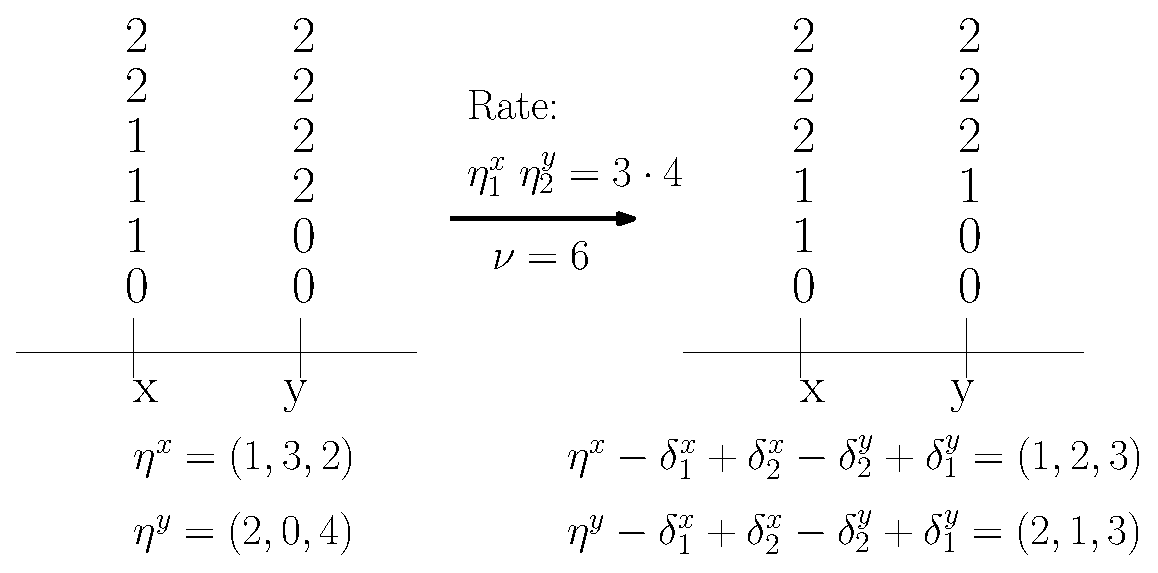
\includegraphics[scale=0.45]{BulkStirring.eps}
%    \caption{The edge dynamics. Maximal occupation is $\nu=6$. A particle of type $2$ is removed in $x$ and placed in $y$. A particle of type $3$ is removed in $y$ and placed in $x$. This transition occurs at rate $n_{2}^{x}n_{3}^{y}=2\cdot 3$.}
%    \label{fig:1}
%\end{figure}
%\begin{figure}[h]
%    \centering
%    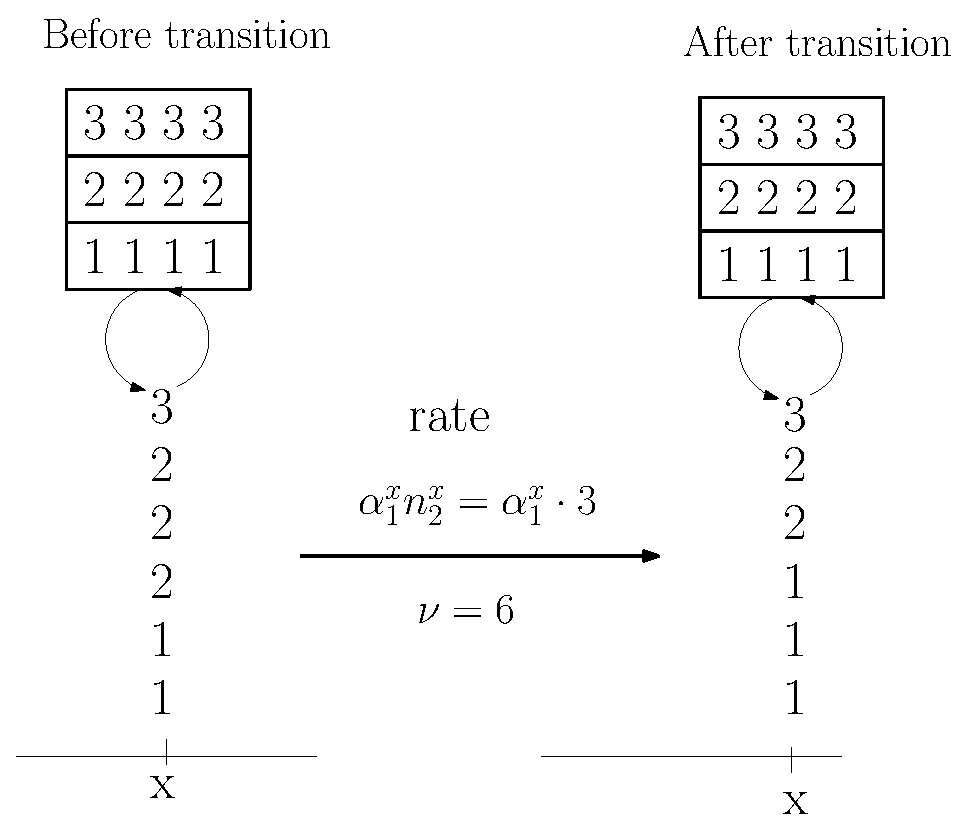
\includegraphics[scale=0.4]{BoundaryStirring.eps}
%    \caption{The site dynamics. Here the maxiaml occupation is $\nu=6$. The reservoir, represented by a square "box" containing all types of particles, remove a type $2$ from site $x$ and replace it with a type $3$. This transition occurs at rate $\alpha_{3}^{x}n_{2}^{x}$.}
%    \label{fig:2}
%\end{figure}
\subsection{Reversible measures (equilibrium)}
For a particular choice of the reservoir parameters one has an $N$-parameter family of reversible measures. More precisely
when the parameters are the same on each site, i.e.
\begin{equation}\label{reversibilityCondition}
\alpha_{a}^{x}=\alpha_{a}\qquad \forall x\in V\,,
\end{equation}
then the process described by the generator \eqref{Generator} is reversible with respect to the 
homogeneous product measure 
\begin{equation}
\label{reversibleMeasure}
\mu_{rev}=\bigotimes_{x\in V}\mu_{rev}^{x}
\end{equation}
with marginals $\mu_{rev}^{x}$ given by 
\begin{equation}
 \mu^{x}_{rev}\sim \text{Multinomial}\left(\twoj,\rho_{1},\ldots,\rho_{N}\right)\,.
\end{equation}
Here
 $$
\rho_{a}=\frac{\alpha_{a}}{|\alpha|}\co
$$
is the density of specie $a$ and we used the notation $|\alpha|=\sum_{a=1}^{N}\alpha_{a}$. Explicitly, 
\begin{equation}
\mu_{rev}^{x}(n^{x})=\frac{\nu!}{\prod_{a=1}^{N}n_{a}^{x}!}\prod_{a=1}^{N}\rho_{a}^{n_{a}^{x}}\,.
\end{equation}
This can be proved  by checking that detailed balance is satisfied. 
If condition \eqref{reversibilityCondition} is not met, then reversibility is lost: each reservoir at site $x$ wants to fix its own set of densities $\rho^{x}=(\rho_{1}^{x},\ldots,\rho_{N}^{x})$ with
 $$
\rho_{a}^x=\frac{\alpha_{a}}{|\alpha^x|}
$$
and  $|\alpha^x|=\sum_{a=1}^{N}\alpha_{a}$. 
Currents will arise when at least two reservoirs have different densities. 

\subsection{Lie algebraic description}

In this paper we will often use the fact that the Markov generator of the multispecies stirring process can be described in terms a Lie algebra of rank $N$.
In this section we provide details about this.

Consider the Lie algebra $gl(N)$ with generators denoted by $\EE_{ab}$ with $a,b\in \{1,\ldots,N\}$ and commutation relations
\begin{equation}\label{eq:comgl}
\left[\EE_{ab},\EE_{cd}\right]=\EE_{ad}\delta_{cb}-\EE_{cb}\delta_{ad}\qquad \forall a,b\in \{1,\ldots,N\}\,.
\end{equation}
The finite-dimensional representations are labelled by partitions $\lambda=(\lambda_1,\lambda_2,\ldots,\lambda_N)$ of $\nu$ with  $\lambda_i\geq \lambda_{i+1}$,  $\lambda_i\in \mathbb{N}$ and $\sum_{i=1}^N \lambda_i = \nu\in\mathbb{N}$.  
We are interested in the {\em symmetric} finite-dimensional representations with 
\begin{equation}\label{eq:dynkin}
    \lambda=(\twoj,0,\ldots,0) \;.
    %\qquad\text{where}\qquad \twoj\in\mathbb{N}\,.
\end{equation} 
The dimension $M_\twoj$ of this symmetric representations is given by the combination of $N$ objects in $\twoj$ positions with repetition, namely
\begin{equation}
	M_\twoj= \frac{(N+\twoj-1)!}{\twoj  !(N-1)!}\dt
\end{equation} 
The generators of the symmetric representations will be denoted by $E_{ab}$.
A basis of the vector space $\mathbb{C}^{M_\twoj}$ are the column vectors denoted by
\begin{equation}
  |n\rangle=  |n_{1},\ldots,n_{N}\rangle,\quad \text{with}\quad n_{i}\in\mathbb{N}_{0}\quad \text{sucht that}\quad \sum_{i=1}^{N}n_{i}=\nu\,.
\end{equation}
%where $\sum_{a=1}^{N}n_{i}=\nu$. 
{\color{red}
The basis vectors satisfy the orthogonality relation with respect to the Euclidean scalar product 
\begin{equation}\label{ortho}
   \langle m|n \rangle =\langle m_{1},\ldots,m_{N}|n_{1},\ldots,n_{N}\rangle=\prod_{a=1}^{N}\delta_{\xi_{a},n_{a}}\co
\end{equation}
where  $ \langle m_{1},\ldots,m_{N}|$ is the row vectors obtained by transposing $|m_{1},\ldots,m_{N}\rangle$ and $\delta_{\xi_{a},n_{a}}$ is the Kronecker delta. 
}
The explicit action of the algebra generators on the basis  vectors $|n\rangle$ is the following:
\begin{equation}\label{actionE}
	\begin{cases}
		E_{ab}|n_{1},\ldots,n_{a},\ldots,n_{b},\ldots,n_{N}\rangle =n_{b}|n_{1},\ldots,n_{a}+1,\ldots,n_{b}-1,\ldots,n_{N}\rangle\qquad\qquad a\neq b\\[0.1cm]
		E_{aa}|n_{1},\ldots,n_{a},\ldots,n_{N}\rangle = n_{a} |n_{1},\ldots,n_{a},\ldots,n_{N}\rangle\dt
	\end{cases}
\end{equation}  
The matrices defined in this way satisfy the commutation relations \eqref{eq:comgl} and yield Dynkin weight \eqref{eq:dynkin}. \\
%{\color{red} Is this remark relevant for us?}
%\newline 
%\textbf{Remark}: it is possible to define these matrices in terms of creation and annihilation operators: see Appendix \ref{appA}.
\\ \\
\textbf{Remark}: The symmetric representations $\lambda=(\twoj,0,\ldots,0)$ are dual to the representations $\lambda=(\twoj,\ldots,\twoj,0)$ that can be obtained via 
\begin{equation}
   \bar E_{ab}=\nu\delta_{ab}-E_{N-b+1,N-a+1}\dt
\end{equation}
{\color{red} This needs to be checked and give alternative form of Hamiltonian?}\\
The process with generator \eqref{Generator} can be described in terms of $gl(N)$ Lie algebra generators. The state space \eqref{stateSpace} is given by the $|V|$-fold tensor product of the vector space with basis elements $|n^x\rangle$ at a given site. Namely,
a vector $|{\bf n}\rangle \in \Omega$ can be written as
%We now define the equivalent of \eqref{stateSpace} in the vector notation
% \begin{equation}
%	\Omega':=\left\{|n\rangle=|n_{1},\ldots,n_{N}\rangle \;:\;n\in\mathbb{N}_0^N,\;\;|n|=\twoj\right\}^{\otimes|V|}
%	\end{equation}
%where we denote 
\begin{equation}
|{\bf n}\rangle=\left(\,\bigotimes_{x\in V}	|n_{1}^{x},\ldots,n_{N}^{x}\rangle\right)
\end{equation}
%where we require that $n_{a}^{x}\in \mathbb{N}_{0}$ and $\forall x\in V$ we have 
with $\sum_{a=1}^{N}n_{a}^{x}=\nu$ for any $x\in V$. Sometimes it will bw convenient to write $|n^{x}\rangle$ to denote, for a fixed $x\in V$, the vector $|n_{1}^{x},\ldots,n_{N}^{x}\rangle$.
{\color{red}
The following orthogonality relation is a consequence of the single site relation \eqref{ortho}
\begin{equation}
    \langle {\bf n}|{\bf m}\rangle =\prod_{x\in V}\prod_{a=1}^N\delta_{n^x_a,m^{x}_a}\,.
\end{equation}
}

We introduce the Hamiltonian operator
\begin{equation}\label{OriginalHamiltonian}
	\begin{split}
		H=\sum_{(x,y)\in \mathcal{E}}\omega_{x,y}\mathcal{H}_{x,y}+\sum_{x\in V}\Gamma_{x}H_{x}
	\end{split}
\end{equation}
where the edge Hamiltonian that describes the interaction between two connected sites is
\begin{equation}\label{edgeHamiltonian}
\mathcal{H}_{x,y}=\sum_{a,b=1}^{N}\Big(E_{ab}^{x} E_{b a}^{y}-E_{bb}^{x} E_{aa}^{y}\Big)
 \end{equation}
  and where the site Hamiltonian is
 \begin{equation}\label{siteHamiltonian}
H_{x}=\sum_{a,b=1}^{N}\alpha_{a}^{x}\left(E_{ab}^{x}-E_{bb}^{x}\right)
\end{equation}
Here $E_{ab}^{x}$ is a copy of $E_{ab}$ defined in \eqref{actionE} acting on site $x$ (and
acting trivially as the identity on the other sites). 
Following  \cite{belitsky2015self}, the Hamiltonian and the Markov generator are linked by
\begin{equation}\label{Hamiltonian-Generator}
H=\mathcal{L}^{T}\dt
\end{equation}
The action of the generator can also be expressed as 
\begin{equation}
    \mathcal{L}f( {\bf n})=\langle f|H| {\bf n}\rangle
\end{equation}
where 
\begin{equation}
    \langle f|=\sum_{ {{\bf m}\in \Omega}}f( {\bf m})\langle  {\bf m}|
\end{equation}

We can write the edge Hamiltonian \eqref{edgeHamiltonian} as a function of the coproduct of the {\color{red} quadratic} Casimir of $gl(N)$
\begin{equation}\label{secondCasimir}
    C=\sum_{a,b=1}^{N}E_{ab}E_{ba}
\end{equation}
that acts diagonally as $C|\bm{n}\rangle=\twoj(\twoj+N)|\bm{n}\rangle$ and belogs to the center of $gl(N)$ (i.e. it commutes with all the algebra elements).  
More precisely,  considering the standard coproduct 
\begin{equation}
\begin{split}
\Delta:gl(N)&\to gl(N)\otimes gl(N)\\
E_{ab}&\to E_{ab}\otimes \mathbbm{1}+\mathbbm{1}\otimes E_{ab}
\end{split}
\end{equation}
we have 
\begin{equation}
\Delta(C)=\sum_{a,b=1}^{N}\Delta(E_{ab})\Delta(E_{ba})=2\sum_{a,b=1}^{N}E_{ab}\otimes E_{ba}+C\otimes \mathbbm{1}+\mathbbm{1}\otimes C\,.
\end{equation}
Then, one can check that 
\begin{equation}\label{hamiltonianCasimir}
	\mathcal{H}_{x,y}=\frac{1}{2}\Delta_{x,y}(C)-\twoj(2\twoj+N)
\end{equation}
where $\Delta_{x,y}(C)$ denotes a copy of $\Delta(C)$ acting on  the sites of edge $(x,y)\in \mathcal{E}$ and acting trivially on the other sites of the graph.


\begin{comment}
We introduce the Hamiltonian operator

\begin{equation}\label{OriginalHamiltonian}
	\begin{split}
		H=\sum_{x,y\in \mathcal{E}}\omega_{x,y}\mathcal{H}_{x,y}+\sum_{x\in V}\Gamma_{x}H_{x}
	\end{split}
\end{equation}
where the edge Hamiltonian is
\begin{equation}\label{edgeHamiltonian}
\mathcal{H}_{x,y}=\sum_{a,l=1}^{N}E_{al}^{x}\otimes E_{la}^{y}-E_{ll}^{x}\otimes E_{aa}^{y}
 \end{equation}
 and where the site Hamiltonian is
 \begin{equation}\label{siteHamiltonian}
H_{x}=\sum_{a,l=1}^{N}\alpha_{a}^{x}\left(E_{al}^{x}-E_{ll}^{x}\right)
\end{equation}
Here $E_{al}^{x}$ is a copy of $E_{al}$ defined in \eqref{actionE} acting on site $x$. 

We can write this Hamiltonian in function of the coproduct of the second Casimir
\begin{equation}
    C_{2}=\sum_{a,b=1}^{N}E_{ab}E_{ba}
\end{equation}
It reads
\begin{equation}
	\mathcal{H}_{x,y}=\left\{\frac{1}{2}\Delta^{xy}(C_{2})-\twoj(2\twoj+N)\frac{1}{2}\mathbbm{1}^{x}\otimes\mathbbm{1}^{y}\right\}
\end{equation}
Here we introduced the standard coproduct
\begin{equation}
\begin{split}
\Delta:gl(N)&\to gl(N)\otimes gl(N)\\
E_{ab}&\to E_{ab}\otimes \mathbbm{1}+\mathbbm{1}\otimes E_{ab}
\end{split}
\end{equation} acting on sites $x,y$ and used that $C_{2}|n\rangle=\twoj(\twoj+N)|n\rangle$. 
\end{comment}
 
\subsection{Integrable process on a line segment}\label{subsection-description-process-LINE}
In this section we specialize the multi-species stirring process to the geometry of the one dimensional chain with sites $\{1,\ldots,L\}$ where two reservoirs act at the boundary sites $1$ and $L$. These reservoirs, exchanging particle with the external environment, put the chain out of equilibrium. The Hamiltonian that we consider here is obtained from \eqref{OriginalHamiltonian} assuming that the conductances are
\begin{equation}
	\omega_{x,y}=\begin{cases}
		1 \quad \text{if}\quad |x-y|=1\\
		0\quad \text{otherwise}
	\end{cases}
\end{equation}
and the coupling to reservoirs are
\begin{equation}
	\Gamma_{x}=\begin{cases}
		1\quad \text{if} \quad x\in \{1,L\}\\
		0\quad \text{otherwise}
	\end{cases}
\end{equation}
We further assume that the maximal occupancy in each site is $\nu=1$, i.e. that there is an \textit{hard-core interaction}.
We will denote the element of the representation of the $gl(N)$  Lie algebra with $\nu=1$ by lowercase letters, i.e. $(e_{ab})_{a,b\in\{1,\ldots,N\}}$, to highlight that we are in the first fundamental representation of the algebra.
The Hamiltonian now reads
\begin{equation}\label{hamiltonian}
	H=H_{left}+H_{bulk}+H_{right}
\end{equation}
where
\begin{equation}
	H_{bulk}=\sum_{x=1}^{L-1}\mathcal{H}_{x,x+1}
\end{equation}
Here $\mathcal{H}_{x,x+1}$  is a copy (acting on the vertices of the edge $x,x+1$) of the two-site Hamiltonian
\begin{equation}\label{H-corsivo}
	\begin{split}
		\mathcal{H}=P-\id
	\end{split}
\end{equation}
with 
\begin{equation}
	P=\sum_{a,b=1}^Ne_{ab}\otimes e_{ba}.
\end{equation} 
The action of $\mathcal{H}$ amounts to the permutation of the occupations of the two sites, i.e.
\begin{equation}
	\begin{split}
		\mathcal{H}|n\rangle\otimes   |m\rangle&=|m\rangle \otimes |n\rangle-|n\rangle \otimes|m\rangle\dt
	\end{split}
\end{equation}
The boundary terms are given by 
\begin{equation}
	H_{left}=\begin{pmatrix}
		\alpha_{1}-1&\alpha_{1}&\alpha_{1}&\ldots&\ldots&\alpha_{1}\\
		\alpha_{2}&\alpha_{2}-1&\alpha_{2}&\ldots&\ldots&\alpha_{2}\\
		\vdots&\vdots& &\ddots& &\vdots\\
		\alpha_{N-1}&\alpha_{N-1}&\ldots&\ldots&\alpha_{N-1}-1&\alpha_{N-1}\\
		\alpha_{N}&\alpha_{N}&\ldots&\ldots&\alpha_{N}&\alpha_{N}-1
	\end{pmatrix}
\end{equation}
\begin{equation}
	H_{right}=\begin{pmatrix}
		\beta_{1}-1&\beta_{1}&\beta_{1}&\ldots&\ldots&\beta_{1}\\
		\beta_{2}&\beta_{2}-1&\beta_{2}&\ldots&\ldots&\beta_{2}\\
		\vdots&\vdots& &\ddots& &\vdots\\
		\beta_{N-1}&\beta_{N-1}&\ldots&\ldots&\beta_{N-1}-1&\beta_{N-1}\\
		\beta_{N}&\beta_{N}&\ldots&\ldots&\beta_{N}&\beta_{N}-1
	\end{pmatrix}
\end{equation}
where, without loss of generality,  we assume that the parameters satisfy
\begin{equation}\label{ratesConditions}
	\sum_{a=1}^{N}\alpha_{a}=1,\qquad\sum_{a=1}^{N}\beta_{a}=1\;.
\end{equation} 
We define also 
\begin{equation}\label{lambdaConditions}
	\lambda_{a}=\alpha_{a}-\beta_{a}\quad\text{with}\quad \sum_{a=1}^{N}\lambda_{a}=0\,.
\end{equation}
Under these assumption the Hamiltonian \ref{hamiltonian} is integrable (see \cite{vanicat2017exact} for its derivation within the Quantum Inverse Scattering method). 


\section{Duality}\label{sectionDuality}
\subsection{Definition}
Consider two Markov processes $(\eta_{t})_{t\geq 0}$ defined on a state space $\Omega$ and $(\xi_{t})_{t\geq 0}$ defined on a state space $\widetilde{\Omega}$. We say that they are dual, with respect to a duality function $D:\Omega\times \widetilde{\Omega}\to \mathbb{R}$, if $\forall \eta\in\Omega$, $\forall \xi\in\widetilde{\Omega}$ and $\forall t> 0$ we have 
\begin{equation}\label{duality-expectation}
    \mathbb{E}_{\eta}\left[D(\eta_{t},\xi)\right]=\mathbb{E}_{\xi}\left[D(\eta,\xi_{t})\right]
\end{equation}
where $\mathbb{E}_{\eta}$ denotes the expectation with respect to the law of the Markov process $(\eta_{t})_{t\geq 0}$ initialized with the particle configuration $\eta$, whereas $\mathbb{E}_{\xi}$ denotes the expectation with respect to the law of the Markov process $(\xi_{t})_{t\geq 0}$ initialized with the particle configuration $\xi$.
The duality definition can also be formulated as a relation between the generators. Call $\mathcal{L}$ the generator of $(\eta_{t})_{t\geq0}$ and $\widetilde{\mathcal{L}}$ the generator of $(\xi_{t})_{t\geq 0}$, then we say that these two processes are dual with respect to the duality function $D:\Omega\times \widetilde{\Omega}\to \mathbb{R}$ if $\forall \eta\in\Omega$ and $\forall \xi\in\widetilde{\Omega}$
\begin{equation}\label{dualityRelationGenerator}
    \left(\mathcal{L}D(\cdot,\xi)\right)(\eta)=\left(\widetilde{\mathcal{L}}D(\eta,\cdot)\right)(\xi)
\end{equation}
In the specific case where $\mathcal{L}=\widetilde{\mathcal{L}}$ we say that the process is self-dual.
\newline
\newline
\textbf{Remark}:
when the state spaces of the dual processes is finite, the generators and the duality function can be represented as matrices with elements $\mathcal{L}(\eta,\eta^{'})$, $\widetilde{\mathcal{L}}(\xi,\xi^{'})$ and $D(\eta,\xi)$ for arbitrary $\eta,\eta^{'}\in\Omega$ and $\xi,\xi^{'}\in \widetilde{\Omega}$. Therefore, we can write the duality relation \eqref{dualityRelationGenerator} as 
\begin{equation}
    \sum_{\eta^{'}\in\,\Omega}\mathcal{L}(\eta,\eta^{'})D(\eta^{'},\xi)=\sum_{\xi^{'}\in\, \widetilde{\Omega}}\widetilde{\mathcal{L}}(\xi,\xi^{'})D(\eta,\xi^{'})
\end{equation}
that can be read as
\begin{equation}\label{dualityIntertwines}
    \mathcal{L}D=D\widetilde{\mathcal{L}}^{\,T}
\end{equation}
where the superscript $T$ denotes the matrix transposition. Therefore, the duality relation \eqref{dualityIntertwines} is an intertwining between two linear operators $\mathcal{L}$ and $\widetilde{\mathcal{L}}$. Working in terms of the Hamiltonian operators the duality relation \eqref{dualityIntertwines} reads 
\begin{equation}\label{DualityRelation}
    H^{T}D=D\widetilde{H}\dt
\end{equation}
\subsection{Duality for the multi-species stirring process}\label{statementDualitySubsection}
In this section we formulate duality for the multi-species stirring process $(\bm{n}(t))_{t\geq 0}$, defined by the generator \eqref{Generator}.
The dual  process $(\bm{\xi}(t))_{t\geq 0}$ is defined on the \textit{enlarged graph} $\widetilde{G}=(\widetilde{V},\widetilde{\mathcal{E}})$ where 
\begin{equation}
	\widetilde{V}:=V\cup \left\{u(x)\,:\, x\in V\right\}\qquad \widetilde{\mathcal{E}}:=\mathcal{E}\cup \left\{(x,u(x))\,:\, x\in V\right\}\dt
\end{equation}
This means that to each site $x\in V$ we associate an ``extra-site'', denoted $u(x)$. The configuration space of the dual process is the enlarged state space
\begin{equation}\label{dualStateSpace}
    \widetilde{\Omega}= \bigtimes_{x\in V} \widetilde{\Omega}_{x}\ = \bigtimes_{x\in V} (\Omega_{x}\times \mathbb{N}_{0}^{N})\dt
\end{equation}
Dual particle will accumulate in these extra-sites in the course of time. We write the configurations $\bm{\xi} \in \widetilde\Omega$  as
\begin{equation}
    \bm{\xi}=\left(\xi_{1}^{x},\ldots,\xi_{N}^{x},\xi_{1}^{u(x)},\ldots,\xi_{N}^{u(x)}\right)_{x\in V}
\end{equation}
where the component $\xi_{a}^{x}$ is interpreted as the number of dual particles of type $a\in \{1,\ldots,N\}$ at site $x$, 
and the component $\xi_{a}^{u(x)}$  gives the number of dual particles of type $a\in \{1,\ldots,N\}$ at 
the extra-site $u(x)$ connected to $x\in V$.

The duality function is given by
\begin{equation}\label{dualityElements}
	D(\bm{n},\bm{\xi})=\prod_{x\in V}\left(\frac{(\nu -\sum_{a=1}^{N-1}\xi_{a}^{x})!}{\nu!}\prod_{a=1}^{N-1}\frac{n_{a}^{x}!}{(n_{a}^{x}-\xi_{a}^{x})!}\left(\rho_{a}^{x}\right)^{\xi_{a}^{u(x)}}\,\right)
\end{equation}
where we denote the \textit{density} of the species $a\in \{1,\ldots,N-1\}$ imposed by the reservoir at site $x\in V$  by 
\begin{equation}
\rho_{a}^{x}:=\frac{\alpha_{a}^{x}}{|\alpha^{x}|}\dt
\end{equation}
The dual process is defined by its Markov generator, which reads
 \begin{equation}\label{DualGenerator}
    \widetilde{\mathcal{L}}=\sum_{(x,y)\in \mathcal{E}}\omega_{x,y}\mathcal{L}_{x,y}+\sum_{x\in V}\Gamma_{x}\widetilde{\mathcal{L}}_{x}
\end{equation}
where 
$\mathcal{L}_{x,y}$ is defined in \eqref{edgeGenerator} and, for any function $f:\widetilde{\Omega}\to \mathbb{R}$ 
\begin{equation}\label{siteDualGenerator}
    \widetilde{\mathcal{L}}_{x}f(\bm{\xi})=|\alpha^{x}|\sum_{a=1}^{N-1}\xi_{a}^{x}\left(f(\bm{\xi}-\bm{\delta}_{a}^{x}+\bm{\delta}_{N}^{x}+\bm{\delta}_{a}^{u(x)})-f(\bm{\xi})\right)\dt
\end{equation}
\newline
Therefore the dual dynamics is described as follows. On one hand, the edge part $\mathcal{L}_{x,y}$ of the dual Markov generator gives rise to  the multi-species stirring dynamics on the graph. On the other hand, the site
part $\widetilde{\mathcal{L}}_{x}$ of the dual generator replaces a particle of any type $a\in\{1,\ldots,N-1\}$ at site $x$ with a particle of type $N$ and creates a particle of the same type $a$ at the extra-site $u(x)$. This last transition is performed with rate $|\alpha^{x}|\xi_{a}^{x}$. This means that eventually the dual process voids the graph, putting all the dual particles of species $\{1,\ldots,N-1\}$ in the extra-sites. In other words the extra-sites play the role of absorbing boundaries. 
\newline \newline
\textbf{Remark}: in the reversible situation, i.e. when $\forall x\in V$ we have $\rho_{a}^{x}=\rho_{a}$, the expectation  of the duality function  $D(\bm{n},\bm{\xi})$ with   $\bm{n}$ distributed as  $\mu_{rev} = \bigtimes_{x\in V}\text{Multinomial}\left(\twoj, \rho_{1},\ldots,\rho_{N}\right)$ is
\begin{equation}
\mathbb{E}_{\mu^{rev}}\left[D(\bm{n},\bm{\xi})\right]=\prod_{a=1}^{N-1}\left(\rho_{a}\right)^{\sum_{x\in V}\xi_{a}^{x}+\sum_{x\in V}\xi_{a}^{u(x)}}\qquad \forall \bm{n}\in \Omega,\quad\forall \bm{\xi}\in \widetilde{\Omega}\dt
\end{equation}

\subsection{Proof of duality}
To prove duality between $(\bm{n}(t))_{t\geq 0}$ and $(\bm{\xi}(t))_{t\geq 0}$ we  show that \eqref{dualityIntertwines} is fulfilled.  To show this, we will use the Hamiltonians (linked with the Markov generators by \eqref{Hamiltonian-Generator}) and their Lie algebraic description. Indeed, in this formalism the proof reduces to finding symmetries and group like transformation of generators of the Lie algebra.\\
To a configuration $\bm{\xi}$ of the configuration space  \eqref{dualStateSpace} of a dual process we associate the vector
\begin{equation}
    |\bm{\xi}\rangle=\bigotimes_{x\in V}\left(|\xi_{1}^{x},\ldots,\xi_{N}^{x}\rangle\otimes |\xi_{1}^{u(x)},\ldots,\xi_{N}^{u(x)}\rangle\right)\dt
\end{equation}
The Hamiltonian of the dual process reads
\begin{equation}\label{DualHamiltonian}
    \widetilde{H}=\sum_{x,y\in \mathcal{E}}\omega_{x,y}\mathcal{H}_{x,y}+\sum_{x\in V}\Gamma_{x}\widetilde{H}_{x}
\end{equation}
where $\mathcal{H}_{x,y}$ is the one defined in \eqref{edgeHamiltonian}, while 
\begin{equation}\label{siteDualHamiltonian}
    \widetilde{H}_{x}=|\alpha^{x}|\sum_{a=1}^{N-1}\left((a^{\dagger})_{a}^{u(x)}\,E_{Na}^{x}-E_{aa}^{x}\right)\dt
\end{equation}
Here we introduced bosonic creation operator $a^{\dagger}$ acting on the left-hand-side as $\langle q|a^{\dagger}=\langle q+1|$ on a generic vector $\langle q|$ with $q\in \mathbb{N}_{0}$, so that in \eqref{siteDualHamiltonian} 
$(a^{\dagger})_{a}^{u(x)}$ denotes a copy of $a^{\dagger}$ acting on the extra-site $u(x)$ and on the species $a\in\{1,\ldots,N-1\}$. \\
We will show below that the Hamiltonians \eqref{OriginalHamiltonian} and \eqref{DualHamiltonian} are dual in the sense of \eqref{DualityRelation}. The duality matrix $D$ is described as 
\begin{equation}\label{dualityMatrix}
    D=\prod_{x\in V}d_{x}\otimes \dd
\end{equation}
where
\begin{equation}\label{bulkElementDualityMatrix}
d_{x}=R_{x}\exp{(E^{x})}
\end{equation}
with 
\begin{equation}\label{EquationEx}
E^{x}=\sum_{a=1}^{N-1}E_{aN}^{x}
\end{equation}
and
\begin{equation}\label{Revmatrix}
    R_{x}=\sum_{n^{x}\in\Omega_{x}}\frac{\prod_{a=1}^{N}n_{a}^{x}!}{\nu!}|n_{1}^{x},\ldots,n_{N}^{x}\rangle\langle n_{1}^{x},\ldots,n_{N}^{x}|
\end{equation}
and where 
\begin{equation}\label{dualityMatrix2}
\dd=\sum_{\xi_{1}^{u(x)},\ldots,\xi_{N-1}^{u(x)}=0}^{\infty}\prod_{a=1}^{N-1}\left(\rho_{a}^{x}\right)^{\xi_{a}^{u(x)}}\langle \xi_{1}^{u(x)},\ldots,\xi_{N}^{u(x)}|\dt
\end{equation}
The matrix $R_{x}$ is diagonal. Its elements are related to the inverse of the weights of the reversible measure \eqref{reversibleMeasure}. In particular, to obtain these elements, we have considered the weights of \eqref{reversibleMeasure} when all the parameters $p_{i}=\frac{1}{N}$. Then, the constant $\left(\frac{1}{N}\right)^{\nu}$ has been neglected, since it does not change the duality relation. This $R_{x}$ is called the ``cheap'' duality matrix (see \cite{giardina2009duality}). \\
Since \eqref{dualityMatrix} is product over sites, proving \eqref{DualityRelation} is equivalent to showing that 
\begin{equation}\label{edgeDualRealtion}
    \mathcal{H}_{x,y}^{T}D=D\mathcal{H}_{x,y}\qquad \forall (x,y)\in \mathcal{E}
\end{equation}
and 
\begin{equation}\label{siteDualRelation}
    H_{x}^{T}D=D\widetilde{H}_{x}\qquad \forall x\in V.
\end{equation}
We perform the proof of duality in three steps: first we will show that matrix \eqref{dualityMatrix} has elements \eqref{dualityElements}; second we will prove \eqref{edgeDualRealtion}; finally we will show \eqref{siteDualRelation}. 
As a preliminary result we note that 
\begin{equation}\label{transpositionPropertyR}
(E_{ba}^{x})^{T}=R_{x}E_{ab}^{x}R_{x}^{-1}\qquad \forall x\in V
\end{equation}
that follows immediately from the definition of $E_{ab}$. 
\begin{comment}

\begin{align*}
R_{x}E_{ab}^{x}R_{x}^{-1}=&\sum_{r^{x}\in\Omega_{x}}\frac{\xi_{1}^{x}!\ldots r_{N}!}{\nu!}|\xi_{1}^{x},\ldots,\xi_{N}^{x}\rangle \langle \xi_{1}^{x},\ldots, \xi_{N}^{x}|
	\\&
	\sum_{s^{x}\in \Omega_{x},}s_{b}^{x}|s_{1}^{x},\ldots,s_{a}^{x}+1,\ldots,s_{b}^{x}-1,\ldots s_{N}^{x}\rangle \langle s_{1}^{x},\ldots,s_{N}^{x}|
	\\&
	\sum_{n^{x}\in\Omega_{x}}\frac{\nu!}{n_{1}!\ldots n_{N}!}|n_{1}^{x},\ldots,n_{N}^{x}\rangle \langle n_{1}^{x},\ldots, n_{N}^{x}|
 \\=&\sum_{r^{x}\in \Omega_{x}}
	\xi_{a}^{x}|\xi_{1}^{x},\ldots,\xi_{N}^{x}\rangle \langle \xi_{1}^{x},\ldots,\xi_{a}^{x}-1,\ldots,r_{b}^{x}-1,\ldots,\xi_{N}^{x}|
	\\=&
	\left(E_{ba}^{x}\right)^{T}
\end{align*}
where in the up to last equation we used the orthogonality relation \eqref{ortho}. 
\end{comment}
\paragraph{Elements of the duality matrix.}We aim to show that 
\begin{equation}\label{proofDualityElements}
\langle \bm{n}|D|\bm{\xi}\rangle=D(\bm{n},\bm{\xi})\qquad   \forall \bm{n}\in \Omega,\quad \bm{\xi}\in \widetilde{\Omega}
\end{equation}
with $D(\bm{n},\bm{\xi})$ defined in \eqref{dualityElements}. 
Fix an arbitrary site $x\in V$, then we have that 
\begin{align*}
	 &\langle n^{x}|d_{x}\otimes \dd|\xi^{x}\rangle\\=&\langle n_{1}^{x},\ldots,n_{N}^{x}| (\exp{(E_{N1}^{x}+\ldots+E_{N\,N-1}^{x}}))^{T}R_{x}\otimes\sum_{q_{1}^{u(x)},\ldots,q_{N-1}^{u(x)}=0}^{\infty}\prod_{a=1}^{N-1}\left(\rho_{a}^{x}\right)^{q_{a}^{u(x)}}\langle q_{1}^{u(x)},\ldots,q_{N}^{u(x)}|
	 \\&|\xi_{1}^{x},\ldots,\xi_{N}^{x}\rangle \otimes |\xi_{1}^{u(x)},\ldots,\xi_{N}^{u(x)}\rangle
\end{align*}
where we used \eqref{transpositionPropertyR}. \\
On one hand, on the extra-site $u(x)$ we have 
\begin{align*}
\sum_{q_{1}^{u(x)},\ldots,q_{N-1}^{u(x)}=0}^{\infty}\prod_{a=1}^{N-1}\left(\rho_{a}^{x}\right)^{q_{a}^{u(x)}}\langle q_{1}^{u(x)},\ldots,q_{N}^{u(x)}|\xi_{1}^{u(x)},\ldots,\xi_{N}^{u(x)}\rangle=\prod_{a=1}^{N-1}\left(\rho_{a}^{x}\right)^{\xi_{a}^{u(x)}}
\end{align*}
where we used the orthogonality relation \eqref{ortho}. 
On the other hand, on the site $x$, we have 
\begin{align*}
&\langle n_{1}^{x},\ldots,n_{N}^{x}|(\exp{(E_{N1}^{x}+\ldots+E_{N\,N-1}^{x})})^{T}R_{x}|\xi_{1}^{x},\ldots,\xi_{N}^{x}\rangle\\&= \langle  n_{1}^{x},\ldots,n_{N}^{x}|\left(\sum_{k_{1}=0}^{\infty}\frac{\left\{\left(E_{N1}^{x}\right)^{T}\right\}^{k_{1}}}{k_{1}!}\ldots\sum_{k_{N-1}=0}^{\infty}\frac{\left\{\left(E_{N\,N-1}^{x}\right)^{T}\right\}^{k_{N-1}}}{k_{N-1}!}\sum_{s\in\Omega_{x}}\frac{s_{1}^{x}!\ldots s_{N}^{x}!}{\nu!}|s_{1}^{x},\ldots,s_{N}^{x}\rangle\langle s_{1}^{x},\ldots,s_{N}^{x}|\right)
\\&
\hspace{2.cm}\qquad|\xi_{1}^{x},\ldots,\xi_{N}^{x}\rangle
\\&=
\sum_{k_{1}=0}^{n_{1}^{x}}\ldots\sum_{k_{N-1}=0}^{n_{N-1}^{x}}\langle n_{1}^{x}-k_{1},\ldots,n_{N-1}^{x}-k_{N-1},n_{N}^{x}+k_{1}+\ldots+k_{N-1}|
\\&
\hspace{2.cm}\prod_{a=1}^{N-1}\left((n_{a}^{x}(n_{a}^{x}-1)\ldots (n_{a}^{x}-k_{a}+1)\right)\frac{1}{k_{1}!,\ldots,k_{N-1}!}\frac{\xi_{1}^{x}!\ldots \xi_{N}^{x}!}{\nu!}|\xi_{1}^{x},\ldots,\xi_{N}^{x}\rangle
\\&=
\sum_{k_{1}=0}^{n_{1}^{x}}\ldots\sum_{k_{N-1}=0}^{n_{N-1}^{x}}\langle n_{1}^{x}-k_{1},\ldots,n_{N-1}^{x}-k_{N-1},\ldots,n_{N}^{x}+k_{1}+\ldots+k_{N-1}|\frac{n_{1}^{x}!\ldots n_{N-1}^{x}!}{(n_{1}^{x}-k_{1})!\ldots(n_{N-1}^{x}-k_{N-1})!}
\\& 
\hspace{2.cm}\qquad\frac{1}{k_{1}!,\ldots,k_{N-1}!}\frac{\xi_{1}^{x}!\ldots \xi_{N}^{x}!}{\nu!}|\xi_{1}^{x},\ldots,\xi_{N}^{x}\rangle
\\&=
\frac{(\nu-\sum_{a=1}^{N-1}\xi_{a}^{x})}{\nu!}\prod_{a=1}^{N-1}\frac{n_{a}^{x}!}{(n_{a}^{x}-\xi_{a}^{x})!}
\end{align*}
where in the last equality we applied the orthogonality relations \eqref{ortho} and the fact that $\xi_{N}^{x}=\nu-\sum_{a=1}^{N-1}\xi_{a}^{x}$. Finally, by taking the product over $x\in V$ \eqref{proofDualityElements} is proved.
\begin{flushright}
    $\square$
\end{flushright}
\paragraph{Proof of \eqref{edgeDualRealtion}.}To show this relation we need two 'ingredients'. First the existence of a similarity transformation between the Hamiltonian $\mathcal{H}_{x,y}$  and its transposed. As we will show, this similarity transformation is $R_{x}R_{y}$.  Second, the possibility of finding a symmetry for the edge Hamiltonian. Exploiting \eqref{hamiltonianCasimir}, we will search for a symmetry of the second Casimir $C_{2}$. As we will see, this symmetry is $\sum_{a=1}^{N-1}E_{aN}$ \\
We first look for the similarity between $\mathcal{H}_{x,y}$ and its transposed. Using \eqref{transpositionPropertyR} we obtain 
 
\begin{equation}\label{transpositionPropertyH}
    \mathcal{H}_{x,y}^{T}=\left(R_{x}R_{y}\right)\mathcal{H}_{x,y}\left(R_{x}R_{y}\right)^{-1}
\end{equation}
therefore we have found the similarity transformation between $\mathcal{H}_{x,y}$ and its transposed. \\
We now look for a symmetry of $\mathcal{H}_{x,y}$, i.e. a matrix $S_{x,y}$ of the same dimension such that it satisfies 
\begin{equation}
	\mathcal{H}_{x,y}S_{x,y}=S_{x,y}\mathcal{H}_{x,y}\quad \Leftrightarrow \quad [\mathcal{H}_{x,y},S_{x,y}]=0\dt
\end{equation}
Using \eqref{hamiltonianCasimir}, we observe that $\mathcal{H}_{x,y}$ is proportional to the coproduct of the second Casimir, up to a diagonal term. Therefore, it is enough to look for a symmetry of $\Delta (C_{2})$. Using the bilinearity of the coproduct operator and the fact that $C_{2}$ belongs to the centre of the Lie algebra, it is easy to show that for any matrix $E\in gl(N)$ it holds
\begin{equation}
	[C_{2},E]=0\quad \Rightarrow\quad \left[\Delta (C_{2}),\Delta(E)) \right]=0\dt
\end{equation}
We chose 
\begin{equation}
	E=\sum_{a=1}^{N-1}E_{aN}
\end{equation}
and, for a fixed $(x,y)\in \mathcal{E}$, we define
\begin{equation}
	S_{x,y}=\exp{(\Delta^{x,y}(E))}=\exp{(E^{x})}\exp{(E^{y})}
\end{equation}
where $\Delta^{x,y}(E)$ is a copy of the coproduct acting on sites $x$ and $y$. Therefore, this operator $S_{x,y}$ satisfies
\begin{equation}\label{symmetryH}
	\left[S_{x,y},\mathcal{H}_{x,y}\right]=0
\end{equation}
i.e. it is a symmetry of $\mathcal{H}_{x,y}$. \\ Exploiting these considerations we write


\begin{comment}
As already pointed out, $\mathcal{H}_{x,y}$ is a linear function of $\Delta(C_{2})$. This implies that symmetries of  $\Delta(C_{2})$ are also symmetries of  $\mathcal{H}_{x,y}$. Moreover, the coproduct is a Lie algebra homomorphism, i.e. $\forall A,B\in gl(N)$
\begin{equation}\label{symmetryCoproduct}
    [A,B]=0\quad \Longrightarrow\quad \left[\Delta(A),\Delta(B)\right]=0
\end{equation}
This tells us that it is enough to find a symmetry of $C_{2}$. This element belongs to the center of $gl(N)$, and therefore it commutes with all the element of this algebra. Consider
\begin{equation}\label{equationE}
    E=\sum_{a=2}^{N}E_{a1}
\end{equation}
To obtain a product structure of the elements of the duality matrix, we introduce
\begin{equation}
    S=\exp{(\Delta(E))}
\end{equation}
Finally, for fixed $(x,y)\in \mathcal{E}$, we define
\begin{equation}
    S_{x,y}=\exp{(\Delta^{x,y}(E))}=\exp{(E^{x})}\exp{(E^{y})}
\end{equation}
where $\Delta^{x,y}(E)$ is a copy of the coproduct acting on sites $x$ and $y$. This operator $S^{x,y}$ satisfies
\begin{equation}\label{symmetryH}
    \left[S_{x,y},\mathcal{H}_{x,y}\right]=0
\end{equation}
i.e. $S_{x,y}$ is a symmetry of $\mathcal{H}_{x,y}$. \\ Exploiting these considerations we write
\end{comment}
\begin{equation}
    \begin{split}
        \mathcal{H}_{x,y}^{T}D&=(R_{x}R_{y})\mathcal{H}_{x,y}(R_{x}R_{y})^{-1}\left(d_{x}\otimes\dd\right)\left(d_{y}\otimes\mathcal{D}_{\widehat{y}}\right)\prod_{z\in V\,:\, z\neq x,y}\left(d_{z}\otimes \mathcal{D}_{\widehat{z}}\right)
        \\&=\left(R_{x}\exp{(E^{x})}\otimes \dd\right)\left(R_{y}\exp{(E^{y})}\otimes \mathcal{D}_{\widehat{y}}\right)\mathcal{H}_{x,y}\prod_{z\in V\,:\, z\neq x,y}\left(d_{z}\otimes \mathcal{D}_{\widehat{z}}\right)
        \\&=
        D\mathcal{H}_{x,y}
    \end{split}
\end{equation}
 where we used \eqref{transpositionPropertyH} and \eqref{symmetryH} in the second equality. Thus, \eqref{edgeDualRealtion} is proved. 
 %\textbf{Reamrk}: it is important to notice that the elements of the duality matrix \eqref{dualityElements} are well defined only if at each site $x\in V$ and for every species $a\in \{2,\ldots,N\}$ the number of dual particles $r_{x}^{a}$ is lower or equal than the number of original particles $n_{a}^{x}$. This implies that the dynamics of the dual process is simpler, because described by a lower number of particles. By the way, it is possible to perform computations similar to the one made in this proof choosing instead of  \eqref{equationE} {\color{red} $E=\sum_{a=2}^{N}E_{1a}$ or $E=\sum_{a=2}^{N}E_{aa}$.}
 %{\color{blue} That's confusing. What is E?}
 
 
% However, they would lead to duality matrices where the number of dual particles is greater than the number of original ones, loosing the simplification of the dynamics of the dual process. 
 \begin{flushright}
     $\square$
 \end{flushright}
 \paragraph{Proof of \eqref{siteDualRelation}.} To prove \eqref{siteDualRelation} we need to transform via the Hadamard formula the transposed of the site Hamiltonian \eqref{siteDualHamiltonian} and then to  introduce properly a creation operator acting on an extra-site $u(x)$. % that we connect to every site $x\in V$ of the graph $G$. \\
 Considering $A,B\in gl(N)$, the Hadamard formula reads 
 \begin{equation}\label{HadamardFormula}
     \exp{(-B)}A\exp{(B)}=A-\left[B,A\right]+\frac{1}{2!}\left[B,\left[B,A\right]\right]-\frac{1}{3!}\left[B,\left[B,\left[B,A\right]\right]\right]+\ldots
 \end{equation}
In the following we need the application of the Hadamard formula with $B=\sum_{a=1}^{N-1}E_{aN}$ defined in \eqref{EquationEx} and with $A$ equal to some of the generator $E_{cd}$ of the Lie algebra with $c,d\in\{1,\ldots,N\}$. Therefore we compute 
\begin{align}
	\left[B,A\right]=\sum_{a=1}^{N-1}\left[E_{aN},E_{cd}\right]=\delta_{cN}\sum_{a=1}^{N-1}E_{ad}-\delta_{d<N}E_{cN}
\end{align}
and 
\begin{align}
	\left[B\left[B,A\right]\right]=&\left[\sum_{a=1}^{N-1}E_{aN},\delta_{cN}\sum_{b=1}^{N-1}E_{bd}-\delta_{d<N}E_{cN}\right]\nonumber\\=&
	\sum_{a=1}^{N-1}\left(\delta_{cN}\sum_{b=1}^{N-1}\left[E_{aN},E_{bd}\right]-\delta_{d<N}\left[E_{aN},E_{cN}\right]\right)\nonumber\\=&
	\sum_{a=1}^{N-1}\left(-\delta_{cN}\delta_{ad}\sum_{b=1}^{N-1}E_{bN}-\delta_{d<N}\delta_{cN}E_{aN}\right)\nonumber\\=&
	-\left(\delta_{cN}\delta_{d<N}+\delta_{d<N}\delta_{cN}\right)\sum_{b=1}^{N-1}E_{bN}\nonumber
	\\=&
	-2\delta_{cN}\delta_{d<N}\sum_{b=1}^{N-1}E_{bN}
\end{align}
From the third commutator on we always obtain zero. All in all we have that 
 \begin{align}\label{HT-BA}
 	\exp{\left(-\sum_{a=1}^{N-1}E_{aN}\right)}E_{cd}\exp{\left(\sum_{a=1}^{N-1}E_{aN}\right)}=E_{cd}-\delta_{cN}\sum_{a=1}^{N-1}E_{ad}+\delta_{d<N}E_{cN}-\delta_{cN}\delta_{d<N}\sum_{b=1}^{N-1}E_{bN}\dt
 \end{align}
\begin{comment}
\begin{enumerate}
    \item for $A=E_{b N}$ with $b\in \{1,\ldots,N-1\}$, we obtain 
    \begin{equation}\label{HT_El1}
        \exp{(-E)}E_{b N}\exp{(E)}=E_{b N}
    \end{equation}
    because $E_{b N}$ commutes with $E$
    \item for $A=E_{bb}$ with $b \in \{1,\ldots,N-1\}$, we obtain 
    \begin{equation}\label{HT_Ell}
        \exp{(-E)}E_{b b}\exp{(E)}=E_{b b}+E_{b N}
    \end{equation}
Indeed, using \eqref{eq:comgl} we have 
    \begin{equation}
       \left[E, E_{bb}\right]=\sum_{a=1}^{N-1}\left(E_{ab}\delta_{b N}-E_{b N}\delta_{ab}\right)=-E_{bN}
    \end{equation}
    Inserting the above commutator in \eqref{HadamardFormula}, we obtain \eqref{HT_Ell}.
    \item for $A=E_{Nb}$ with $b\in \{1,\ldots,N-1\}$, we obtain 
    \begin{equation}\label{HT-E1l}
        \exp{(-E)}E_{N a}\exp{(E)}=E_{Na}+E_{NN}-\sum_{c=1}^{N-1}\left(E_{cN}+E_{ca}\right)
    \end{equation}
  %\com{Why indices have names $b, k, j, a, b$? Fix one set for the generators}
    
    Indeed, using \eqref{eq:comgl} we have 
    \begin{equation}
[E,E_{Na}]=\sum_{c=1}^{N-1}\left(E_{ca}\delta_{NN}-E_{NN}\delta_{ca}\right)= (\sum_{c=1}^{N-1}E_{ca} ) -E_{NN};
\end{equation}
and 
\begin{equation}
\begin{split}
\left[E,[E,E_{Na}]\right]&=\sum_{d=1}^{N-1}\sum_{c=1}^{N-1}\left[E_{dN},E_{ca}\right]-\sum_{d=1}^{N-1}\left[E_{dN},E_{NN}\right]
\\&=
\sum_{d,c=1}^{N-1}\left(E_{da}\delta_{cN}-E_{cN}\delta_{da}\right)-\sum_{d=1}^{N-1}\left(E_{dN}\delta_{NN}-E_{NN}\delta_{dN}\right)
\\=&
-2\sum_{c=1}^{N-1}E_{cN};
\end{split}
\end{equation}
therefore we have that 
\begin{equation}
	content...
\end{equation}
Inserting the above commutators in \eqref{HadamardFormula}, we obtain \eqref{HT-E1l}.
\item for $A=E_{ba}$ with $a,b \in \{1,\ldots,N-1\}$ we obtain 
\begin{equation}\label{HT-Ekl}
    \exp{(-E)}E_{a b}\exp{(E)}=E_{ba}+E_{bN}
\end{equation}
   Indeed, using \eqref{eq:comgl} we have 
\begin{equation}
[E,E_{ba}]=\sum_{c=1}^{N-1}\left(E_{ca}\delta_{b1}-E_{bN}\delta_{c a}\right)=-E_{bN};
\end{equation}
Inserting the above commutator in \eqref{HadamardFormula}, we obtain \eqref{HT-Ekl}.
\item for $A=E_{NN}$ we obtain 
\begin{equation}\label{HT-E11}
    \exp{(-E)}E_{NN}\exp{(E)}=E_{NN}-\sum_{a=1}^{N-1}E_{aN}
\end{equation}
  Indeed, using \eqref{eq:comgl} we have 

\begin{align*}
[E,E_{NN}]=\sum_{c=1}^{N-1}\left(E_{cN}\delta_{NN}-E_{NN}\delta_{cN}\right)=\sum_{c=1}^{N-1}E_{cN};
\end{align*}
  Inserting the above commutator in \eqref{HadamardFormula}, we obtain \eqref{HT-E11}.
\end{enumerate}
\end{comment}
Using \eqref{transpositionPropertyR} we write the transpose of site Hamiltonian \eqref{siteHamiltonian} 
\begin{equation}
    \begin{split}
H_{x}^{T}=\sum_{a,b=1}^{N}\alpha_{a}^{x}\left(E_{ab}^{x}-E_{bb}^{x}\right)^{T}=R_{x}\sum_{a,b=1}^{N}\alpha_{a}^{x}\left(E_{b a}^{x}-E_{bb}^{x}\right)R_{x}^{-1}\dt
    \end{split}
\end{equation}
We multiply both sides by $R_{x}\exp{(E^{x})}$
\begin{equation}\label{intermediateTransposeSite}
    H_{x}^{T}R_{x}\exp{(E^{x})}=R_{x}\sum_{a,b =1}^{N}\alpha_{a}^{x}\left(E_{b a}^{x}-E_{bb}^{x}\right)\exp{(E^{x})}\dt
\end{equation}
%By inserting the identity $I=\exp{(E^{x})}\exp{(-E^{x})}$ and 
By using \eqref{HT-BA} and the fact that the first Casimir operator $C_{1}=\sum_{a,b=1}^{N}E_{ab}$ is central for the algebra we have 
\begin{comment}
then, in the right hand side
\begin{equation}\label{intermediateTransposeSite}
H_{x}^{T}R_{x}\exp{(E^{x})}=R_{x}\exp{(E^{x})}\exp{(-E^{x})}\sum_{a,b=1}^{N}\alpha_{a}^{x}\left(E_{b a}^{x}-E_{bb}^{x}\right)\exp{(E^{x})}
\end{equation}
\end{comment}
%where $E^{x}$ is a copy of $E$ acting on site $x\in V$ and $E_{ab}^{x}$ with $a,b\in \{1,\ldots,N\}$ are copies of $E_{ab}$ acting at site $x\in V$.
% Using 
 \begin{comment}
 \eqref{HT_El1}, \eqref{HT_Ell},\eqref{HT-E1l}, \eqref{HT-Ekl}, \eqref{HT-E11} we have that 
\begin{align}
    &\exp{(-E^{x})}\sum_{a=1}^{N}\sum_{b=1}^{N}\alpha_{a}^{x}\left(E_{b a}^{x}-E_{bb}^{x}\right)\exp{(E^{x})}\nonumber
    \\&=\nonumber
    \sum_{a=2}^{N}\alpha_{a}^{x}\left(E_{Na}^{x}+E_{NN}^{x}-\sum_{c=1}^{N-1}(E_{cN}^{x})-\sum_{c=1}^{N-1}(E_{ca}^{x})-E_{NN}^{x}+
    \sum_{c=2}^{N}(E_{cN}^{x})\right)
    \\&+\nonumber
    \alpha_{N}^{x}\sum_{b=1}^{N-1}\left(E_{bN}^{x}-E_{bb}^{x}-E_{bN}^{x}\right)+\sum_{a=1}^{N-1}\sum_{b=1}^{N-1}\alpha_{a}^{x}\left(E_{ba}^{x}+E_{bN}^{x}-E_{bb}^{x}-E_{bN}^{x}\right)
    \\&=\nonumber
    \sum_{a=1}^{N-1}\alpha_{a}^{x}E_{Na}^{x}-|\alpha^{x}|\sum_{b=1}^{N-1}E_{bb}^{x}=
    \sum_{a=1}^{N-1}\left(\alpha_{a}^{x}E_{Na}^{x}-|\alpha^{x}|E_{aa}^{x}\right)
    \\&=\nonumber
    |\alpha^{x}|\sum_{a=1}^{N-1}\left(\frac{\alpha_{a}^{x}}{|\alpha^{x}|}E_{Na}^{x}-E_{aa}^{x}\right)
    \\&=
    |\alpha^{x}|\sum_{a=1}^{N-1}\left(\rho_{a}^{x}E_{Na}^{x}-E_{aa}^{x}\right)
 \end{align}
in short
\end{comment}
\begin{equation}\label{HadTransfBoundary}
\exp{(-E^{x})}\sum_{a=1}^{N}\sum_{b=1}^{N}\alpha_{a}^{x}\left(E_{b a}^{x}-E_{bb}^{x}\right)\exp{(E^{x})}=	|\alpha^{x}|\sum_{a=1}^{N-1}\left(\rho_{a}^{x}E_{Na}^{x}-E_{aa}^{x}\right)\dt
\end{equation}
Thus, we rewrite \eqref{intermediateTransposeSite} as
\begin{equation}\label{siteHadamardI}
H_{x}^{T}R_{x}\exp{(E^{x})}=R_{x}\exp{(E^{x})}|\alpha^{x}|\sum_{a=1}^{N-1}\left(\rho_{a}^{x}E_{Na}^{x}-E_{aa}^{x}\right)\dt
\end{equation}
Making the tensor product on both sides of \eqref{siteHadamardI} by 
\begin{equation}
\sum_{\xi_{1}^{u(x)},\ldots,\xi_{N-1}^{u(x)}=0}^{\infty}\prod_{a=1}^{N-1}\left(\rho_{a}^{x}\right)^{\xi_{a}^{u(x)}}\langle \xi_{1}^{u(x)},\ldots,\xi_{N}^{u(x)}|
\end{equation}
and we obtain 
\begin{equation}\label{siteHadamardII}
    \begin{split}
&H_{x}^{T}d_{x}\otimes\sum_{\xi_{1}^{u(x)},\ldots,\xi_{N-1}^{u(x)}=0}^{\infty}\prod_{a=1}^{N-1}\left(\rho_{a}^{x}\right)^{\xi_{a}^{u(x)}}\langle \xi_{1}^{u(x)},\ldots,\xi_{N}^{u(x)}|
\\=&
d_{x}\otimes \sum_{\xi_{1}^{u(x)},\ldots,\xi_{N-1}^{u(x)}=0}^{\infty}\prod_{a=1}^{N-1}\left(\rho_{a}^{x}\right)^{\xi_{a}^{u(x)}}\langle \xi_{1}^{u(x)},\ldots,\xi_{N}^{u(x)}|\,|\alpha^{x}|\sum_{a=1}^{N}\left(\rho_{a}^{x}E_{Na}^{x}-E_{aa}\right)\dt
    \end{split}
\end{equation}
Recalling the action of the bosonic creation operator acting at site $u(x)$ and on the species $a\in \{1,\ldots,N-1\}$ we have that 
\begin{equation}\label{bosonicKX}
    \langle \xi_{1}^{u(x)},\ldots,\xi_{a}^{u(x)}+1,\ldots,\xi_{N}^{u(x)}|=  \langle \xi_{1}^{u(x)},\ldots,\xi_{a}^{u(x)},\ldots,\xi_{N}^{u(x)}|(a^{\dagger})^{u(x)}_{a}\dt
\end{equation}
Using \eqref{bosonicKX} by a fixed $a\in \{1,\ldots,N-1\}$ we rewrite the term of \eqref{siteHadamardII} with Lie generator $E_{Na}^{x}$ on the right hand side of \eqref{siteHadamardII} as 
\begin{equation}
    \begin{split}
&\sum_{\xi_{1}^{u(x)},\ldots,\xi_{N-1}^{u(x)}=0}^{\infty}\prod_{a=1}^{N-1}\left(\rho_{a}^{x}\right)^{\xi_{a}^{u(x)}}\langle \xi_{1}^{u(x)},\ldots,\xi_{a}^{u(x)},\ldots,\xi_{N}^{u(x)}|\rho_{a}^{x}E_{Na}^{x}
\\=&
\sum_{\xi_{1}^{u(x)},\ldots,\xi_{N-1}^{u(x)}=0}^{\infty}\prod_{a=1}^{N-1}\left(\rho_{a}^{x}\right)^{\xi_{a}^{u(x)}+1}\langle \xi_{1}^{u(x)},\ldots,\xi_{a}^{u(x)}+1,\ldots,\xi_{N}^{u(x)}|(a^{\dagger})_{a}^{u(x)}E_{Na}^{x}
\\=&
\sum_{\xi_{1}^{u(x)},\ldots,\xi_{N-1}^{u(x)}=0}^{\infty}\prod_{a=1}^{N-1}\left(\rho_{a}^{x}\right)^{\xi_{a}^{u(x)}}\langle \xi_{1}^{u(x)},\ldots,\xi_{a}^{u(x)},\ldots,\xi_{N}^{u(x)}|(a^{\dagger})_{a}^{u(x)}E_{Na}^{x}
    \end{split}
\end{equation}
where, in the last equality, we performed a change of summation variable. Therefore, inserting this last equation in \eqref{siteHadamardII} we obtain 
\begin{equation}
    \begin{split}
H_{x}^{T}\left(d_{x}\otimes \dd\right)&=
     H_{x}^{T}d_{x}\otimes \sum_{\xi_{1}^{u(x)},\ldots,\xi_{N-1}^{u(x)}=0}^{\infty}\prod_{a=1}^{N-1}\left(\rho_{a}^{x}\right)^{\xi_{a}^{u(x)}}\langle \xi_{1}^{u(x)},\ldots,\xi_{N}^{u(x)}|
\\&=
d_{x}\otimes \sum_{\xi_{1}^{u(x)},\ldots,\xi_{N-1}^{u(x)}=0}^{\infty}\prod_{a=1}^{N-1}\left(\rho_{a}^{x}\right)^{\xi_{a}^{u(x)}}\langle \xi_{1}^{u(x)},\ldots,\xi_{N}^{u(x)}|\,|\alpha^{x}|\sum_{a=1}^{N-1}\left((a^{\dagger})_{a}^{u(x)}E_{Na}^{x}-E_{aa}^{x}\right)   
\\&=
d_{x}\otimes \sum_{\xi_{1}^{u(x)},\ldots,\xi_{N-1}^{u(x)}=0}^{\infty}\prod_{a=1}^{N-1}\left(\rho_{a}^{x}\right)^{\xi_{a}^{u(x)}}\langle \xi_{1}^{u(x)},\ldots,\xi_{N}^{u(x)}|\widetilde{H}_{x}
\\&=
\left(d_{x}\otimes \dd\right)\widetilde{H}_{x}\dt
    \end{split}
\end{equation}
Since the duality matrix \eqref{dualityMatrix} is product over sites, the above equality implies \eqref{siteDualRelation}. 
\begin{flushright}
$\square$
\end{flushright}
\subsection{Duality for a boundary driven chain}\label{Subsection-ss-nonI}
In this subsection we specialize the results of Subsection \ref{statementDualitySubsection} to a chain of length $L$, where two reservoirs are attached to sites $1$ and $L$. Each site can still host $\nu\geq 1$ particles, chosen among the $N$ types. Now the dual graph is still a chain, but where two extra-sites $0$ (connected to $1$) and $L+1$ (connected to $L$) are present. As already pointed out the dual process eventually voids the graph by piling up particles of species $\{1,\ldots,N-1\}$ in the extra sites ($0$ and $L+1$) and replacing them by types $N$. This property allows to characterize the steady state non-equilibrium distribution (assuming that it is unique) by the probability that dual particles are absorbed in the extra-sites, then called \textit{absorption probabilities}. \\The process $\left(\bm{n}(t)\right)_{t\geq0}$ is defined on the space
 \begin{equation}\label{stateSpace-Chain}
 	\Omega=\bigtimes_{x=1}^{L} \Omega_{x}
 \end{equation} and its generator reads
\begin{equation}
	\mathcal{L}=\mathcal{L}_{left}+\sum_{x=1}^{L-1}\mathcal{L}_{x,x+1}+\mathcal{L}_{right}\dt
\end{equation} 
The bulk is 
\begin{equation}
	\mathcal{L}_{x,x+1}f(\bm{n})=\sum_{a,b=0}^{N}n_{a}^{x}n_{b}^{x+1}\left(f(\bm{n}-\bm{\delta}_{a}^{x}+\bm{\delta}_{b}^{x}+\bm{\delta}_{a}^{x+1}-\bm{\delta}_{b}^{x+1})-f(\bm{n})\right)
\end{equation}
while at the boundaries 
\begin{equation}
	\mathcal{L}_{left}f(\bm{n})=\sum_{a,b=0}^{N}\alpha_{a}n_{b}^{1}\left(f(\bm{n}-\bm{\delta}_{b}^{x}+\bm{\delta}_{a}^{x})-f(\bm{n})\right)\qquad \mathcal{L}_{right}f(\bm{n})=\sum_{a,b=0}^{N}\beta_{a}n_{b}^{L}\left(f(\bm{n}-\bm{\delta}_{b}^{x}+\bm{\delta}_{a}^{x})-f(\bm{n})\right)\dt
\end{equation}
 The process is dual with respect to $(\bm{\xi}(t))_{t\geq0} $ defined on the enlarged configuration space
\begin{equation}\label{stateSpaceDUAL-Chain}	
	\widetilde{\Omega}=N_{0}^{N}\times\bigtimes_{x=1}^{L} \Omega_{x}\times N_{0}^{N}
\end{equation}
whit dual generator
\begin{equation}
	\widetilde{\mathcal{L}}=\widetilde{\mathcal{L}}_{left}+\sum_{x=1}^{L-1}\mathcal{L}_{x,x+1}+\widetilde{\mathcal{L}}_{right}
\end{equation} 
where $\mathcal{L}_{x,x+1}$ is given by \eqref{Generator} and where the boundaries are absorbing, i.e. 
\begin{equation}\label{abs-dual-boundary-chain}
	\begin{split}
		\widetilde{\mathcal{L}}_{left}f(\bm{\xi})&=|\alpha|\sum_{a=1}^{N-1}\xi_{a}^{1}\left(f(\bm{\xi}-\bm{\delta}_{a}^{1}+\bm{\delta}_{N}^{1}+\bm{\delta}_{a}^{0})f(\bm{\xi})\right)\\\widetilde{\mathcal{L}}_{right}f(\bm{\xi})&=|\beta|\sum_{a=1}^{N-1}\xi_{a}^{L}\left(f(\bm{\xi}-\bm{\delta}_{a}^{L}+\bm{\delta}_{N}^{L}+\bm{\delta}_{a}^{L+1})-f(\bm{\xi})\right)
	\end{split}
\end{equation}
where $0$ and $L+1$ are the extra-sites. The duality function reads
\begin{equation}\label{dualityFunctionChain}
	D(\bm{n},\bm{\xi})=\prod_{a=1}^{N-1}\left(\rho_{a}^{L}\right)^{\xi_{a}^{0}}\prod_{x=1}^{L}\frac{(\nu-\sum_{a=1}^{N-1}\xi_{a}^{x})!}{\nu!}\prod_{a=1}^{N-1}\frac{\eta_{a}^{x}!}{(n_{a}^{x}-\xi_{a}^{x})!}\prod_{a=1}^{N-1}\left(\rho_{a}^{R}\right)^{\xi_{a}^{L+1}}
\end{equation}
where $\rho_{\alpha}^{L}=\frac{\alpha_{a}}{|\alpha|}$ and where $\rho_{\alpha}^{R}=\frac{\beta_{a}}{|\beta|}$.\\
The dual process has absorbing boundaries, i.e. all dual particles are eventually absorbed at $0$ or at $L+1$ with a certain probability. This implies that the chain is eventually voided and the steady state correlations of the original process can be written via the absorption probabilities of the dual process as explained in the following. 
We call $\mu_{stat}$ the stationary measure of the the process $(\bm{n}(t))_{t\geq 0}$. Consider an arbitrary initial configuration of $(\bm{n}(t))_{t\geq 0}$ denoted by $\bm{n}$. For every $m\in\{1,\ldots,L\}$ we consider the dual configuration  $\bm{\widehat{\xi}}=\sum_{k=1}\delta_{s_{k}}^{y_{k}}$ with $y_{k}\in\{1,\ldots,L\}$ and $s_{k}\in \{1,\ldots,N-1\}$ for every $k\in \{1,\ldots,m\}$. The following  equalities holds thanks to the duality relation \eqref{duality-expectation}:
\begin{equation}\label{ExptationSS}
	\begin{split}
		\mathbb{E}_{\mu^{stat}}\left[D(\bm{n}(t),\hat{\bm{\xi}})\right]&=\lim_{t\to\infty}\mathbb{E}_{\bm{n}}\left[D(\bm{n}(t),\hat{\bm{\xi}})\right]=\lim_{t\to\infty}\mathbb{E}_{\hat{\bm{\xi}}}\left[D(\bm{n},\bm{\xi}(t))\right]
		\\&=
		\sum_{i_{1}=0}^{|\hat{\xi}_{1}|}\ldots\sum_{i_{N}=0}^{|\hat{\xi}_{N}|}\prod_{a=1}^{N-1}\left(\rho_{a}^{L}\right)^{i_{a}}\left(\rho_{a}^{R}\right)^{|\hat{\xi}_{a}|-i_{a}}\mathcal{P}(i_{1},\ldots,i_{N},\hat{\bm{\xi}})
	\end{split}
\end{equation}
where 
\begin{equation}\label{Pass}
	\mathcal{P}(i_{1},\ldots,i_{N},\hat{\bm{\xi}})	=\mathbb{P}\left(\bm{\xi}(\infty)=\sum_{a=1}^{N-1}\left(i_{a}\delta_{0}+(|\hat{\xi}_{a}|-i_{a})\delta_{L+1}\right)| \bm{\xi}(0)=\hat{\bm{\xi}}\right)
\end{equation}
are called the \textit{absorption probabilities}, i.e. the probabilities that $i_{a}$ particles of species $a$ are absorbed at $0$ and $|\xi_{a}|-i_{a}$ are absorbed at $L+1$ when time goes to infinity and starting from a configuration $\hat{\bm{\xi}}$. Here we denoted $|\hat{\xi}_{a}|=\sum_{x=1}^{L}\hat{\xi}_{a}^{x}$.
The duality function \eqref{dualityFunctionChain} computed in the dual configurations $\bm{\hat{\xi}}$ is given by 
\begin{equation}
	D(\bm{n},\bm{\hat{\xi}})= \frac{\prod_{k=1}^{m}n_{s_{k}}^{y_{k}}}{(\nu-m+1)}\dt
\end{equation}
Therefore, up to a constant, $\mathbb{E}_{\mu^{\text{stat}}}\left[D(\bm{n},\bm{\hat{\xi}})\right]$ gives the non-equilibrium stationary state $m-$points correlations among non-empty species of types $s_{k}\in\{1,\ldots,N-1\}$ situated at sites $y_{k}\in\{1,\ldots,L\}$ with $k\in \{1,\ldots,m\}$. Using \eqref{ExptationSS}, this expectation can be computed by \eqref{ExptationSS} once the absorption probabilities are known. However, these absorption probabilities fulfil some difference equations that are not easy to solve. For example, we report here the solution for the simplest case of one point correlations that is exactly solvable, since the single dual particle behaves as an independent random walker. 
\paragraph{One point correlations for the $\nu\geq 1$ case}
We consider $\widehat{\bm{\xi}}=\delta_{s}^{y}$, then 
\begin{equation}
	\nu D(\eta,\delta_{s}^{y})=n_{s}^{y}\dt
\end{equation}
The average occupation reads
\begin{equation}\label{OnePtsCORR}
	\begin{split}
		\langle n_{s}^{x}\rangle_{\text{stat}}&=\frac{1}{\nu}\lim_{t\to\infty}\mathbb{E}_{\bm{n}}\left[D(\bm{n}(t),\delta_{s}^{y})\right]\\&=\frac{1}{\nu}\sum_{i_{s}=0}^{1}\left(\rho_{s}^{L}\right)^{i_{s}}\left(\rho_{s}^{R}\right)^{1-i_{s}}\mathbb{P}_{\delta_{s}^{y}}\left(\xi_{\infty}=i_{s}\delta_{0}+(1-i_{s})\delta_{L+1}\right)\dt
	\end{split}
\end{equation}
To explicitly find the result, we aim to determine $\mathcal{P}(1,\delta_{s}^{y})=\mathbb{P}_{\delta_{s}^{y}}\left(\xi_{\infty}=i_{s}\delta_{0}+(1-i_{s})\delta_{L+1}\right)$. This is the probability of a random walker on the chain $\{1,\ldots,L\}$ with absorbing boundaries, therefore, it fulfils the following equations discrete Laplace equation
\begin{equation}\label{gamblers-ruin}
	\begin{cases}
		\Delta_{y}^{L}\mathcal{P}(1,\delta_{s}^{y})=0\\
		\mathcal{P}(1,\delta_{s}^{1})=\frac{|\alpha|}{1+|\alpha|}+\mathcal{P}(1,\delta_{s}^{2})\frac{1}{1+|\alpha|}\\
		\mathcal{P}(1,\delta_{s}^{L})=\mathcal{P}(1,\delta_{s}^{L-1})\frac{1}{1+|\beta|}
	\end{cases}
\end{equation}
where $\Delta_{y}^{L}$ is the discrete Laplace operator on the chain of length $L$. The equations \eqref{gamblers-ruin} can be solved and using $\mathcal{P}(1,\delta_{s}^{y})=1-\mathcal{P}(0,\delta_{s}^{y})$ we obtain 
\begin{equation}
	\langle n_{s}^{x}\rangle_{\text{stat}}=\frac{1}{\nu}\frac{\alpha_{s}(L|\beta|-|\beta|x+1)+\beta_{s}(|\alpha|x+1-|\alpha|)}{|\alpha||\beta|L-|\alpha||\beta|+|\alpha|+|\beta|}\dt
\end{equation}
\textbf{Remark}: In case $|\alpha|=|\beta|=\nu=1$ (when the chain is integrable) we have 
\begin{equation}
	\langle n_{s}^{x}\rangle_{\text{stat}}=\frac{\alpha_{s}(L-x+1)+\beta_{s}x}{L+1}
\end{equation}
that is the same result obtained in \cite{vanicat2017exact}. 
\\
\\ Already for two-point correlations the computations become more involving and hard to solve. In the following we specialize the chain to the integrable case $\nu=1$. As it will be shown, in such a situation the non-equilibrium steady state correlations can be computed with different techniques exploiting the integrability of the process (matrix product ansatz and quantum inverse scattering method) combined with duality and, as a by-product, all absorption probabilities can be explicitly found. 
\subsection{Duality for the integrable process on a line segment}\label{integrableChain-duality}
Here we consider the chain defined in Subsection \ref{subsection-description-process-LINE}. We recall that the geometry is a one dimensional chain with sites $\{1,\ldots,L\}$ where reservoirs are attached to $1$ and $L$. Now we assume the hard-core exclusion rule, i.e. $\nu=1$. The dynamics is described by an Hamiltonian that is written in terms of the first fundamental representation of $gl(N)$. Duality result stated in Subsection \ref{statementDualitySubsection} can be adapted. The extra-sites are denoted by $0$ and $L+1$, and they are connected with sites $1$ and $L$ of the chain respectively. The matrix $R_{x}$ defined in \eqref{Revmatrix} 
reduces to the identity, therefore the relation between the generators of the algebra and its transposed reduces to
\begin{equation}\label{transpostionPropertyFund}
	e_{ab}^T= e_{ba}\dt
\end{equation}
Therefore, duality matrix reads
\begin{equation}
	D=\mathcal{D}_{0}\otimes\prod_{x=1}^{L}\exp{\left(\sum_{a=1}^{N-1}e_{aN}^{x}\right)}\otimes \mathcal{D}_{L+1}
\end{equation}
where $\mathcal{D}_{0}$ and $\mathcal{D}_{L+1}$ are given in \eqref{dualityMatrix2}. 
The elements of this duality matrix are given by
\begin{equation}\label{ElementsDualityMatrixChain}
	D(\bm{n},\bm{\xi})=\prod_{a=1}^{N-1}\alpha_{a}^{\xi_{a}^{0}}\left(\prod_{x=1}^{L}\prod_{a=1}^{N-1}\mathbbm{1}_{\{n_{a}^{x}\geq \xi_{a}^{x}\}}\right)\prod_{a=1}^{N-1}\beta_{a}^{\xi_{a}^{L+1}}\dt
\end{equation}
The dual Hamiltonian is
\begin{equation}
	\widetilde{H}=\widetilde{H}_{left}+\sum_{x=1}^{L-1}\mathcal{H}_{x,x+1}+\widetilde{H}_{right}
\end{equation}
where $\mathcal{H}$ is defined in \eqref{H-corsivo} and 
\begin{equation}\label{boundary-H-dual-chain}
	\widetilde{H}_{left}=\sum_{a=1}^{N-1}\left((a^{\dagger})_{a}^{0}\,E_{Na}^{1}-E_{aa}^{1}\right)\qquad 	\widetilde{H}_{right}=\sum_{a=1}^{N-1}\left((a^{\dagger})_{a}^{L+1}\,E_{Na}^{L}-E_{aa}^{L}\right)\dt
\end{equation}
In the long-time limit the dual process voids the chain, i.e. all particles of types $\{1,\ldots,N-1\}$ are eventually absorbed at the extra-sites $0$ and $L+1$ and replaced by types $N$. We also notice that, up the the bosonic creation operators $(a^{\dagger})_{a}$, the dual boundary Hamiltonians \eqref{boundary-H-dual-chain} are triangular. This simplification will be crucial in Sections \ref{sectionIntegrabiliy} and \ref{Section-Mapping}.\\

Using the above duality elements, we can compute the  $m$-point correlations between non-empty particles using the absorption probabilities. Consider a dual configuration $\bm{\hat{\xi}}:=\sum_{k=1}^{m}\delta_{s_{k}}^{y_{k}}$ where $s_{k}\in\{1,\ldots,N-1\}$ and $y_{k}\in\{1,\ldots,L\}$ such that $y_{k}<y_{k+1}$ for every $k\in\{1,\ldots,m\}$. Fix an arbitrary initial configuration $\bm{n}$, the elements \eqref{ElementsDualityMatrixChain} of the duality matrix computed in the dual configuration $\bm{\hat{\xi}}$ read
\begin{equation}
	D(\bm{n},\bm{\hat{\xi}})=\prod_{k=1}^{m}\mathbbm{1}_{\{n_{s_{k}}^{s_{k}}=1\}}\dt
\end{equation}
Repeating the argument of Subsection \ref{Subsection-ss-nonI} and denoting the $m$-point correlations by $\langle n_{s_{1}}^{y_{1}}\cdots n_{s_{m}}^{y_{m}}\rangle_{stat}$ we have 
%To compute the steady state $m$-point correlations of the process $\bm{n}(t)$ we recall that the dual process eventually voids the chain (by putting all particles in the extra-sites $0$ and $L$). Therefore, we have the following equalities
\begin{equation}\label{CorrelationByABS-prob}
	\begin{split}
	\langle n_{s_{1}}^{y_{1}}\cdots n_{s_{m}}^{y_{m}}\rangle_{stat}&=\lim_{t\to \infty}\mathbb{E}_{\bm{n}}\left[D(\bm{n}(t),\bm{\hat{\xi}})\right]=\lim_{t\to \infty}\mathbb{E}_{\bm{\xi}}\left[D(\bm{n},\bm{\hat{\xi}}(t))\right]
	\\&=\sum_{c_{1}=0}^{1}\ldots \sum_{c_{m}=0}^{1}\prod_{k=1}^{m}\alpha_{a_{k}}^{c_{k}}\beta_{a_{k}}^{1-c_{k}}\mathcal{P}(c_{1},\ldots,c_{m},\hat{\bm{\xi}})
\end{split}
\end{equation}
where
\begin{equation}\label{absProbabilitiesIntegrable}
	\mathcal{P}(c_{1},\ldots,c_{m},\hat{\bm{\xi}}):=\mathbb{P}\left(\bm{\xi}(\infty)=\sum_{k=1}^{m}\left(c_{k}\delta_{0}+(1-c_{k})\delta_{L+1}\right)\lvert \bm{\xi}(0)=\hat{\bm{\xi}}\right)
\end{equation}
 namely the joint probability of having, for all $k=1,\ldots,m$, $c_{k}$ particles of species $s_{k}$ at site $y_{k}$ are absorbed at left and $1-c_{k}$ of the same particles absorbed at right. Therefore, by computing these absorption probabilities we determine the arbitrary non-equilibrium steady state correlations of the integrable multi-species stirring process. 






\section{Exact steady state and correlations for the integrable chain}\label{sectionIntegrabiliy}
In this section we aim to use duality and the matrix product ansatz (MPA) to determine the moments and correlations of the non-equilibrium steady state for the integrable version of the multi-species stirring process, defined in Subsection \ref{integrableChain-duality}. As it will turn out, the commutation relations of the matrix product ansatz allowing to determine a closed formula for all correlations. As a by-product, absorption probabilities can be explicitly found.%, giving a further probabilistic interpretation for the non-equilibrium steady state. 
\subsection{Matrix product ansatz for the non-equilibrium steady state}
The matrix product ansatz has been formulated in \cite{vanicat2017exact}, here we briefly recall it.
 Denoting by $|\Psi(t)\rangle$ the column vector that encodes the probability distribution of the chain with Hamiltonian \eqref{hamiltonian} at time $t\geq 0$, its evolution equation is given by 
 the master equation
\begin{equation}
    \frac{d|{\Psi}(t)\rangle}{dt}=H|{\Psi}(t)\rangle\dt
\end{equation}
This Markov chain is irreducible and positive recurrent, therefore there exists a unique stationary measure, that will be reached when time goes to infinity, regardless of the initial configuration. 
We denote by $|\Psi\rangle$ the column vector that gives the stationary distribution. This vector is the right eigenvector with vanishing eigenvalue of $H$, i.e. it solves 
\begin{equation}\label{definition-SteadyStateH}
	H|\Psi\rangle =0\dt
\end{equation}
The MPA states the following
\begin{equation}
	|\Psi\rangle=\frac{1}{Z_{L}}\langle V^{*}|\begin{pmatrix}
		X_{1}\\
		\vdots\\
		X_{N}
	\end{pmatrix}\otimes \ldots\otimes \begin{pmatrix}
		X_{1}\\
		\vdots\\
		X_{N}
	\end{pmatrix}|V\rangle
\end{equation}
with the normalization 
\begin{equation}
	Z_{L}=\langle V^{*}|(X_{1}+\ldots +X_{N})^{L}|V\rangle\dt
\end{equation}
Here the operators $(X_{a})_{a\in \{1,\ldots,N\}}$ fulfil the commutators
\begin{equation}\label{bulk}
	\left[X_{a},X_{b}\right]=\lambda_{a}X_{b}-\lambda_{b}X_{a}\qquad\forall a,b=1,\ldots,N
\end{equation}
and their action on the boundary vectors are
\begin{equation}\label{leftBoundary}
	\langle V^{*}|\left(\alpha_{a}(X_{1}+\ldots+X_{N})-X_{a}\right)=\lambda_{a}\langle V^{*}|\qquad\forall a=1,\ldots,N\co
\end{equation}
\begin{equation}\label{rightBoundary}
	\left(\beta_{a}(X_{1}+\ldots+X_{N})-X_{a}\right)|V\rangle=-\lambda_{a}|V\rangle\qquad\forall a=1,\ldots,N\dt
\end{equation}
Without loss of generality, we further assume that $\langle V^{*}|V\rangle=1$. 
\newline \newline
\textbf{Remark}: Only $N-1$ of the $N$ equations \eqref{leftBoundary}  are independent. This can be seen by summing them over the species $a\in \{1,\ldots,N\}$, i.e.
	\begin{equation}
		\sum_{a=1}^{N}	\langle V^{*}|\left(\alpha_{a}(X_{1}+\ldots+X_{N})-X_{a}\right)=0,%\sum_{a=1}^{N}\lambda_{a}\langle V^{*}|=0
	\end{equation}
	and using  \eqref{ratesConditions} and \eqref{lambdaConditions}.
 Similarly for the right boundary  \eqref{rightBoundary} there are only  $N-1$ independent equations.
\subsection{The explicit form of the steady state}\label{subsection-exact}
The MPA gives an abstract form of the steady state in terms of an algebra of operators. This path has been followed in \cite{vanicat2017exact} to find one and two-point correlations. 
Here we follow the same approach. We will show that the existence of absorbing dual process established in Section \ref{sectionDuality} simplifies substantially the  use of commutators in the
computation. The idea is summarized as follows. We define a sequence of similarity transformation such that 
\begin{equation}
	H\;\xleftrightarrow{S_{1}}\;H^{'}\;\xleftrightarrow{S_{2}}\;H^{''}
\end{equation} 
where $H^{'}= S_{1} H S_{1}^{-1} $ has both boundary terms in a triangular form, and $H^{''} = S_{2}H' S_{2}^{-1}$ has the left boundary in a triangular form and the right boundary is diagonal. Using these transformations the commutators \eqref{bulk} and the action on the boundary vectors \eqref{leftBoundary}, \eqref{rightBoundary} become simpler. As a consequence, the steady state $|\Psi^{''}\rangle$ of $H^{''}$ can be written explicitly. Finally, reversing the transformations we can retrieve $|\Psi\rangle$.

The first transformation $S_{1}$ is closely related to the duality matrix and we will see that $H^{'}$ is $\widetilde{H}^{T}$, up to the extra-site term described by the bosonic creation operator in \eqref{siteDualHamiltonian}. Therefore, $H^{'}$ is not stochastic. The second transformation $S_{2}$ diagonalizes the right boundary. Finally, the composition  $S_{2} S_{1}$ allows to simplify the commutators of the MPA algebra. \\

The computation are organized as follows: we first define the similarity transformations $S_{1},S_{2}$ and the Hamiltonians $H^{'},H^{''}$. Second, we compute right eigenvector with vanishing eigenvalue of $H^{''}$ exploiting the simpler commutators. Finally, we invert the similarities and retrieve the right eigenvector of $H^{'}$ with vanishing eigenvalue and  the arbitrary correlations in the non-equilibrium steady state. The explicit expression of the steady state $|\Psi\rangle$ of $H$ is reported in Appendix \ref{appB}. 




\begin{comment}
{\color{blue}We aim to find an explicit for for the steady state $|\Psi\rangle$. The MPA gives the steady state in terms of an abstract algebra of operators. If an explicit representation of $(X_{a})_{a=1,\ldots,N}$ was available, it would be possible to compute explicitly all the correlations and currents of particles for the Hamiltonian \eqref{hamiltonian}. Another way of computing this steady state, without passing through a representation, is using the commutators \eqref{bula} and the actions \eqref{leftBoundary} and \eqref{rightBoundary}. For the one and two point correlation and for the currents this has been done in \cite{vanicat2017exact}. Inspired by this last reference, in this subsection, we aim to find exact formulas for the steady state  $|\Psi\rangle$ using only the \eqref{bula}, \eqref{leftBoundary} and \eqref{rightBoundary}. In subsection \ref{correlation-section}, this result will leads to exact correlation for arbitrary number of particles of type $\{2,\ldots,N\}$. This aim will be achieved by the help of a similarity transformation $\mathcal{S}$ that makes commutation relations simpler, and allows to find the steady state $|\widetilde\Psi\rangle$ of a transformed Hamiltonian, denoted  $\mathbb{H}$, with lower-triangular left boundary and diagonal right boundary. Therefore, inverting this similarity, one can retrieve the steady state of \eqref{hamiltonian}. A fundamental 'ingredient' of these computation is duality, that has been proved in section~\ref{sectionDuality}. Indeed, the similarity transformation $\mathcal{S}$ relies on an "intermediate transformation" $V$ (see \eqref{transformationV}) that is, up to the diagonal operator $R$, the duality matrix.} \com{clarify}
\end{comment}
\subsubsection{The similarity transformations}\label{subsectionSTransf}
Consider the matrices
\begin{align}
	\mathcal{S}_{1}:=\exp{\left(\sum_{a=1}^{N-1}e_{Na}\right)}\label{S1Gen}\co\\
	\mathcal{S}_{2}:=\exp{\left(-\sum_{a=1}^{N-1}\beta_{a}e_{aN}\right)}\dt\label{S2Gen}
\end{align}
We introduce
\begin{equation}\label{transformationV}
 \mathcal{S}_{1}^{x}:=\exp{\left(\sum_{a=1}^{N-1}e_{Na}^{x}\right)}\co %=\mathbbm{1}+\sum_{a=2}^{N}e_{1a}
\end{equation}
that is composed by a copy of $\mathcal{S}_{1}$ (see \eqref{S1Gen}) acting at site $x$ and with identities acting at all other sites of the chain. 
Observe that $\mathcal{S}_{1}^{x}$ is the transposed of the bulk part of the duality matrix $d_{x}$  at site $x\in \{1,\ldots,L\}$ (see \eqref{bulkElementDualityMatrix}). By taking the product over the chain we define
\begin{equation}\label{S1-Whole}
    S_{1}=\prod_{x=1}^{L}\mathcal{S}_{1}^{x}\dt
\end{equation}
that is related with the duality matrix by 
\begin{equation}
S_{1}=\prod_{x=1}^{L}d_{x}^{T}
\end{equation}
 The transformation $S_{1}$ is invertible. We introduce 
\begin{equation}\label{hatHamiltonian}
   H^{'}:=H^{'}_{left}+H_{bulk}+H^{'}_{right}
\end{equation}
that is related to $H$ by
\begin{equation}\label{similarV}
   H^{'}=S_{1}HS_{1}^{-1}\dt
\end{equation}
The bulk part of the Hamiltonian is left unchanged while the boundaries are given by 
\begin{equation}
	H^{'}_{left}=\sum_{a=1}^{N-1}\left(\alpha_{a}e_{aN}^{1}-e_{aa}^{1}\right)\qquad H^{'}_{right}=\sum_{a=1}^{N-1}\left(\beta_{a}e_{aN}^{L}-e_{aa}^{L}\right)\dt
\end{equation}
Indeed, using \eqref{HadTransfBoundary}, \eqref{ratesConditions} and \eqref{transpostionPropertyFund}, we obtain for the left boundary
\begin{equation}
	\begin{split}
		H_{left}^{'}&=S_{1}H_{left}S_{1}^{-1}=\exp{\left(\sum_{c=1}^{N-1}e_{Nc}^{1}\right)}\sum_{a,b=1}^{N}\alpha_{a}\left(e_{ab}^{1}-e_{bb}^{1}\right)\exp{\left(-\sum_{c=1}^{N-1}e_{Nc}^{1}\right)}
		\\&=
		\left\{\exp{\left(-\sum_{c=1}^{N-1}e_{cN}^{1}\right)}\sum_{a,b=1}^{N}\alpha_{a}\left(e_{ba}^{1}-e_{bb}^{1}\right)\exp{\left(\sum_{c=1}^{N-1}e_{cN}^{1}\right)}\right\}^{T}
		\\&=
		\sum_{a=1}^{N-1}\left(\alpha_{a}e_{Na}^{1}-e_{aa}^{1}\right)^{T}
		\\&=
		\sum_{a=1}^{N-1}\left(\alpha_{a}e_{aN}^{1}-e_{aa}^{1}\right)\dt
	\end{split}
\end{equation}
Similarly, for the right boundary we have 
\begin{equation}
H_{right}^{'}=\exp{\left(\sum_{c=1}^{N-1}e_{1N}^{L}\right)}\sum_{a,b=1}^{N}\alpha_{a}\left(e_{ab}^{L}-e_{bb}^{L}\right)\exp{\left(-\sum_{c=1}^{N-1}e_{Nc}^{L}\right)}=\sum_{a=1}^{N-1}\left(\beta_{a}e_{aN}^{L}-e_{aa}^{L}\right)\dt
\end{equation}
\textbf{Remark:} The boundary Hamiltonians $H_{left}^{'}$ and $H_{right}^{'}$ relates to the transposed of  $\widetilde{H}_{left}$ and $\widetilde{H}_{right}$, i.e. to the transposed of the boundary part of the dual Hamiltonian  defined in \eqref{siteDualHamiltonian}. They are obtained replacing the  extra-site bosonic creation operators $(a^{\dagger})_{a}^{0}$  (resp. $(a^{\dagger})_{a}^{L+1}$) with the corresponding reservoir parameters $\alpha_a$ (resp. $\beta_a$).
\newline\newline
We have the following correspondence between eigenvectors with zero eigenvalues
\begin{equation}\label{S1-Inverse}
	|\Psi\rangle =S_{1}^{-1}|\Psi^{'}\rangle
\end{equation}
where $|\Psi^{'}\rangle$ satisfies $H^{'}|\Psi^{'}\rangle=0$.

We introduce
 \begin{equation}
 	\mathcal{S}_{2}^{x}:=\exp{\left(-\sum_{a=1}^{N-1}\beta_{a}e_{aN}^{x}\right)}\co%=\mathbbm{1}-\sum_{a=2}^{N}\beta_{a}e_{a1}
 \end{equation}
that is composed by a copy of $\mathcal{S}_{2}$ (see \eqref{S2Gen}) acting at site $x$ and with identities acting at all other sites of the chain. 
Therefore, by taking the product over the chain we obtain 
\begin{equation}\label{S2-Whole}
	S_{2}=\prod_{x=1}^{L}S_{2}^{x}\dt
\end{equation}
We define 
\begin{equation}\label{HSecond}
	H^{''}=H_{left}^{''}+H_{bulk}+H_{right}^{''}\co
\end{equation}
that is related to $H'$ by
\begin{equation}
	H^{''}=S_{2}H^{'}S_{2}^{-1}\dt
\end{equation}
The boundary Hamiltonians of $H^{''}$ read
\begin{align}\label{tri-diag-boundaryHamiltonians}
	H_{left}^{''}=e_{NN}^{1}-\mathbbm{1}+\sum_{a=1}^{N-1}(\alpha_{a}-\beta_{a})e_{aN}^{1}\qquad H_{right}^{''}=e_{NN}^{L}-\mathbbm{1}\dt
\end{align}
The left one is lower triangular and depends on the differences between the boundary parameters, while the right one is diagonal. Equations \eqref{tri-diag-boundaryHamiltonians} are proved using the Hadamard formula \eqref{HadamardFormula} with $B=\sum_{c=1}^{N-1}\beta_{c}e_{cN}$ and $A_{N}=e_{aN},$ and $A_{a}=e_{aa}$.
\begin{comment}
 We compute
\begin{enumerate}
	\item $A_{N}=e_{aN}$ with $a\neq 1$
	\begin{equation}
		\exp{\left(-\sum_{c=1}^{N-1}\beta_{c}e_{cN}\right)}e_{aN}\exp{\left(\sum_{c=1}^{N-1}\beta_{c}e_{cN}\right)}=e_{aN}
	\end{equation}
\item $A_{a}=e_{aa}$ with $a\neq 1$
\begin{equation}
		\exp{\left(-\sum_{c=1}^{N-1}\beta_{c}e_{cN}\right)}e_{aa}\exp{\left(\sum_{c=1}^{N}\beta_{c}e_{cN}\right)}=e_{aa}+\beta_{a}e_{aN}
	\end{equation}
Indeed 
\begin{equation}
	\sum_{c=1}^{N-1}[e_{cN},e_{aa}]=\sum_{c=1}^{N-1}\beta_{c}\left(e_{ca}\delta_{aN}-e_{aN}\delta_{ca}\right)=-\beta_{a}e_{aN}
\end{equation}
\end{enumerate}
\end{comment}
Therefore, using \eqref{HT-BA} we obtain for the left boundary 
\begin{equation}
	\begin{split}
		H_{left}^{''}&=S_{2}H_{left}^{'}S_{2}^{-1}=\exp{\left(-\sum_{c=1}^{N-1}\beta_{c}e_{cN}^{1}\right)}\sum_{a=1}^{N-1}\left(\alpha_{a}e_{aN}^{1}-e_{aa}^{1}\right)\exp{\left(-\sum_{c=1}^{N-1}\beta_{c}e_{cN}^{1}\right)}
		\\&=
		\sum_{a=1}^{N-1}\left(\alpha_{a}e_{aN}^{1}-e_{aa}^{1}-\beta_{a}e_{aN}^{1}\right)
		\\&=
		e_{NN}^{1}-\mathbbm{1}+\sum_{a=1}^{N-1}(\alpha_{a}-\beta_{a})e_{aN}^{1}\dt
	\end{split}
\end{equation}
Similarly, using again \eqref{HT-BA} we have for the right boundary 
\begin{equation}
	\begin{split}
			H_{right}^{''}&=S_{2}H_{right}^{'}S_{2}^{-1}=\exp{\left(-\sum_{c=1}^{N-1}\beta_{c}e_{cN}^{L}\right)}\sum_{a=1}^{N-1}\left(\beta_{a}e_{aN}^{L}-e_{aa}^{L}\right)\exp{\left(-\sum_{c=1}^{N-1}\beta_{c}e_{cN}^{L}\right)}
			\\&=
			\sum_{a=1}^{N-1}\left(\beta_{a}e_{aN}^{L}-e_{aa}^{L}-\beta_{a}e_{aN}^{L}\right)=
			\\&=
			e_{NN}^{L}-\mathbbm{1}\dt
	\end{split}
\end{equation}
The relation between eigenvectors with vanishing eigenvalue is 
\begin{equation}\label{S2-Inverse}
	|\Psi^{'}\rangle = S_{2}^{-1}|\Psi^{''}\rangle
\end{equation}
and $|\Psi^{''}\rangle$ solves
\begin{equation}\label{steadyS-SECOND-def}
	H^{''}|\Psi^{''}\rangle=0\dt
\end{equation}
It is convenient to introduce also the transformation
\begin{equation}\label{similarity}
	S=S_{2}S_{1}=\prod_{x=1}^{L}\exp{\left(-\sum_{a=1}^{N-1}\beta_{a}e_{aN}^{x}\right)}\exp{\left(\sum_{a=1}^{N-1}e_{aN}^{x}\right)}\dt
\end{equation}
This matrix $S$ connects $H$ with $H^{''}$ by 
\begin{equation}
H=S^{-1}H^{''}S
\end{equation}
and, the relation between eigenvectors with vanishing eigenvalue is
\begin{equation}
	|\Psi\rangle=S^{-1}|\Psi^{''}\rangle\dt
\end{equation}

\begin{comment}
Using \eqref{transformationV} we introduce the \textit{similarity transformation} 
\begin{equation}\label{similarity}
    S:=\sum_{a=2}^{N}\beta_{a}\sum_{b=1}^{N}e_{ab}+V=-\sum_{a=2}^{N}\beta_{a}\sum_{b=1}^{N}e_{ab}+\exp{\left(\sum_{a=2}^{N}e_{1a}\right)}
\end{equation}
Taking the tensor product over the sites of the chain we further define
\begin{equation}
    \mathcal{S}:=S^{\otimes L}
\end{equation}
Therefore, we call
\begin{equation}\label{bbHamiltonian}
    \mathbb{H}=\mathbb{B}_{1}+H_{bulk}+\mathbb{B}_{L}
\end{equation}
such that 
\begin{equation}\label{similarS}
    H=\mathcal{S}^{-1} \mathbb{H}\mathcal{S}
\end{equation}
The Hamiltonian $\mathbb{H}$ has lower-triangular left boundary and diagonal right boundary, i.e.
\begin{equation}
    \mathbb{B}_{1}=SB_{1}S^{-1}=e_{11}-\mathbbm{1}+\sum_{a=2}^{N}\left(\alpha_{a}-\beta_{a}\right)e_{a1}=\begin{pmatrix}
		0&0&\ldots&0&0\\
		\alpha_{2}-\beta_{2}&-1&\ldots&0&0\\
		\vdots&\vdots&\ddots&\vdots&\vdots\\
		\alpha_{N-1}-\beta_{N-1}&0&\ldots&-1&0\\
		\alpha_{N}-\beta_{N}&0&\ldots&0&-1
	\end{pmatrix}
\end{equation}
and 
\begin{equation}
    \mathbb{B}_{L}=SB_{L}S^{-1}=e_{11}-\mathbbm{1}=\begin{pmatrix}
		0&0&\ldots&0&0\\
		0&-1&\ldots&0&0\\
		\vdots&\vdots&\ddots&\vdots&\vdots\\
		0&0&\ldots&-1&0\\
		0&0&\ldots&0&-1
  \end{pmatrix}
\end{equation}
The bulk part of $\mathbb{H}$ is left unchanged by this transformation, i.e.
\begin{equation}
    \mathcal{H}_{x,x+1}=\left(S\otimes S\right)\mathcal{H}_{x,x+1}\left(S\otimes S\right)^{-1}
\end{equation}
In the following of our analysis it will be useful to have a relation between \eqref{hatHamiltonian} and \eqref{bbHamiltonian}. This relation reads as
\begin{equation}
    \widehat{H}=\mathcal{T}^{-1}\mathbb{H}\;\mathcal{T}
\end{equation}
where
\begin{equation}
    T=\left(S^{-1}\right)^{T}V=\exp{\left(\sum_{a=2}^{N}\beta_{a}e_{1a}\right)}
\end{equation}
and 
\begin{equation}
    \mathcal{T}:=T^{\otimes L}
\end{equation}
Indeed, by imposing equal \eqref{similarV} and \eqref{similarS} we obtain 
\begin{align*}
    		\left(\mathcal{V}^{-1}\right)^{T}\widehat{H}^{T}\mathcal{V}^{T}&=\mathcal{S}\mathbb{H}\mathcal{S}^{-1}\\
		\mathcal{V}\widehat{H}\mathcal{V}^{-1}&=\mathcal{S}^{T}\mathbb{H}^{T}\left(\mathcal{S}^{-1}\right)^{T}\\
		\widehat{H}&=\mathcal{V}^{-1}\mathcal{S}^{T}\mathbb{H}^{T}\left(\mathcal{S}^{-1}\right)^{T}\mathcal{V}\\
		\widehat{H}&=\mathcal{T}^{-1}\mathbb{H}^{T}\mathcal{T}
\end{align*}
Associated with these new Hamiltonians $\widehat{H}$ and $\mathbb{H}$ we define the following steady states
\begin{equation}
	\mathbb{H}|\widetilde{\Psi}\rangle=0\qquad \widehat{H}^{T}|\widehat{\Psi}\rangle=0
\end{equation}
The steady states $|\Psi\rangle$, $|\widehat{\Psi}\rangle$ and $|\widetilde{\Psi}\rangle$ are linked by 
\begin{align}
	|\Psi\rangle=&\left(\mathcal{S}^{-1}\right)|\widetilde{\Psi}\rangle\label{SteadystateTilde}
 \\|\Psi\rangle =&\left((\mathcal{{V}}^{T})^{-1}\right)|\widehat{\Psi}\rangle \label{SteadystateHat}
 \\|\widehat{\Psi}\rangle=&\left(\mathcal{T}^{T}\right)|\widetilde{\Psi}\rangle\label{SteadyStateHatTilde}
\end{align}
In the following subsections we will first compute the steady state $|\widetilde{\Psi}\rangle$. Then, using the transformation $\mathcal{T}$ we will retrieve $|\widehat{\Psi}\rangle$. Finally, using the transformation $\mathcal{V}$ we will find $|\Psi\rangle$. 
\end{comment}
\subsubsection{Explicit formula for $|\Psi^{''}\rangle$}\label{subsectionSSHsec}
\textbf{Notation}: sometimes, in the following, we will denote differently the configuration of this hard-core chain. Each configuration can be written as
\begin{equation}\label{Tau-Notation}
	|\bm{\tau}\rangle=|\tau_{1},\ldots,\tau_{L}\rangle =\begin{pmatrix}
		\tau_{1}\\
		\vdots\\
		\tau_{L}
	\end{pmatrix}
\end{equation}
with $\tau_{x}\in \{1,\ldots,N\}$, $\forall x\in \{1,\ldots,L\}$. This notation is equivalent to the one introduced in Subsection \ref{subsectionGeneratorStr}. Indeed, assume that at site $x$ we have a particle of type $a\in\{1,\ldots,N\} $, then $|n^{x}\rangle$ is composed by zeros but in the component $n_{a}^{x}$ where there is $1$. Therefore, we can uniquely associate  $\tau_{x}=a$ to this $|n^{x}\rangle$, denoting the presence of the species $a$ at site $x$. With this notation, we have that 
\begin{equation}\label{notation}
	|n^{x}\rangle =\tau_{x}\qquad \text{and}\qquad|\bm{n}\rangle=|\bm{\tau}\rangle
\end{equation}
with the meaning explained above. It will be useful to introduce also $\bm{\tau}=(\tau_{x})_{x\in \{1,\ldots,L\}}$. \\
We state the following result: the ground state of the Hamiltonian $H^{''}$ is given by 
\begin{equation}\label{ResulsBasis}
	|\Psi^{''} \rangle=\sum_{\tau_{1},\ldots,\tau_{L}=1}^{N}\frac{\Gamma\left(2+\sum_{x=1}^{L}\delta_{\tau_{x},N}\right)}{\Gamma\left(2+L\right)}\left(\prod_{x=1}^{L}\left[\lambda_{\tau_{x}}\left(1+\sum_{j=x}^{L}\delta_{\tau_{j},N}\right)\right]^{1-\delta_{\tau_{x},N}}\right)|\mathbf{\bm{\tau}}\rangle
\end{equation}
where 
\begin{equation}
    \delta_{\tau_{x},N}:=\begin{cases}
        N\quad \text{if}\quad \tau_{x}=N\\
        0\quad \text{otherwise}
    \end{cases}
\end{equation}
\textbf{Remark}: In case of $N=2$ we introduce $q=\sum_{x=1}^{L}\delta_{\tau_{x},1}$. Moreover, we for each $q\in \{1,\ldots,L\}$ we call $1\leq\ell_{1}<\ldots,\ell_{q}\leq L$ the coordinates where particles of type $1$ are present. By varying $q$, we have a one-to-one mapping with $\bm{\tau}$. Thus, the coefficient of the above formula can be written as
\begin{align}
&\frac{\Gamma\left(2+\sum_{x=1}^{L}\delta_{\tau_{x},2}\right)}{\Gamma\left(2+L\right)}\left(\prod_{x=1}^{L}\left[\lambda_{\tau_{x}}\left(1+\sum_{j=x}^{L}\delta_{\tau_{j},2}\right)\right]^{1-\delta_{\tau_{x},2}}\right)%=\lambda_{1}^{q}\prod_{x=1}^{L}\left(2+L-y_{x}-\sum_{j=x}^{L}\delta_{\tau_{j},1}\right)^{\delta_{\tau_{x},1}}
=\lambda_{1}^{q}\prod_{k=1}^{q}\frac{\left(1+L-\ell_{k}-\sum_{j=x_{k}+1}^{L}\delta_{\tau_{x_{j}},1}\right)}{(2+L-k)}\dt
\end{align}
Therefore, we write 
\begin{equation}
	|\Psi^{''}\rangle=\sum_{q=0}^{L}\sum_{1\leq \ell_{1}<\ldots<\ell_{q}\leq L}\lambda_{1}^{q}\prod_{k=1}^{q}\frac{\left(1+L-\ell_{k}-q+k\right)}{(2+L-k)}|\bm{\ell},q\rangle
\end{equation}
%and the basis vector $|\bm{\tau}\rangle =\bigotimes_{x=1}^{L}|\tau_{x}\rangle$ with $\tau_{x}\in\{1,\ldots,N\}$ denotes the species that occupies the site $i\in \{1,\ldots,L\}$.
\paragraph{Proof of formula \eqref{ResulsBasis}} 
We consider the vector with elements given by the operators of the MPA $(X_{1},\ldots,X_{N})$ and we act on it with the similarity transformation $S=S_{2}S_{1}$ obtaining new operators $(\Xt_{1},\ldots,\Xt_{N})$ that will satisfy simpler commutation relations. 
For the sake of notation 
\begin{equation}
    \begin{pmatrix}
		X_{a}\\ 
		X_{N}
	\end{pmatrix}=\begin{pmatrix}
	    X_{1}\\
     \vdots\\
     X_{N}
	\end{pmatrix}\quad \forall a\in \{1,\ldots,N-1\}
\end{equation}
We define the transformed matrix product operators
\begin{equation}\label{Xtildes2b}
	\begin{pmatrix}
		\Xt_{a}\\ 
		\Xt_{N}
	\end{pmatrix} =S\begin{pmatrix}
		X_{a}\\X_{N}
	\end{pmatrix}=\begin{pmatrix} 
		X_{a}-\beta_{a}(X_{1}+\ldots+X_{N})\\
				X_{1}+\ldots +X_{N}\\
	\end{pmatrix}%=\begin{pmatrix} 
	%	X_{a}-\beta_{a}\Xt_{N}\\ 
		%	X_{1}+\ldots +X_{N}\\
	%\end{pmatrix}
	\qquad \forall a=1,\ldots N-1
\end{equation}
and, we can also reverse the transformation by $S^{-1}$ and get back: 
\begin{equation}\label{Xes}
	\begin{pmatrix}
		X_{a}\\
		X_{N} 
	\end{pmatrix} =S^{-1}\begin{pmatrix}
		\widetilde{X}_{a}\\
		\widetilde{X}_{N}
	\end{pmatrix}=\begin{pmatrix}
		\Xt_{a}+\beta_{a}\Xt_{N}\\ 
		\beta_N\Xt_{N}-(\Xt_{1}+\ldots+\Xt_{N-1})
	\end{pmatrix}\qquad\forall a\in \{1,\ldots,N-1\}
\end{equation}
Summing over $b\in \{1,\ldots,N\}$ in commutation relations \eqref{bulk} we have
\begin{equation} 
	\left[X_{a},\Xt_{N}\right]=\lambda_{a}\Xt_{N}\qquad\forall a=1,\ldots,N
\end{equation}
with $\widetilde{X}_{N}=\widetilde{X}_{1}+\ldots+\widetilde{X}_{1}$, see \eqref{Xtildes2b}. 
Therefore, we obtain the commutation relations for $\Xt_{a}$ 
\begin{equation}\label{commutationsBula}
	\left[\Xt_{a},\Xt_{N}\right]=\lambda_{a}\Xt_{N}\qquad \forall a\in \{1,\ldots,N-1\}
\end{equation}
Moreover using \eqref{Xtildes2b} and \eqref{Xes}, the action of $\Xt_{a}$ on the boundary vectors are given by 
\begin{equation}\label{commLEFT}
	\langle V^{*}|\left(\lambda_{a}\Xt_{N}-\Xt_{a}\right)=\lambda_{a}\langle V^{*}|\qquad\forall a=1,\ldots,N-1
\end{equation}
\begin{equation}\label{commRIGHT}
	\Xt_{a} |V\rangle= \lambda_{a}|V\rangle\qquad\forall a=1,\ldots,N-1
\end{equation} 
Using the transformed operators $(\widetilde{X}_{a})_{a\in\{1,\ldots,N\}}$, the vector $|\Psi^{''}\rangle$ of the matrix product ansatz is written as
\begin{equation}\label{toDetermineTilde}
	|\Psi^{''}\rangle = \frac{1}{Z_{L}}\sum_{\bm{n}\in \Omega}\langle V^{*}|\prod_{x=1}^{L}\prod_{a=1}^{N}\widetilde{X}_{a}^{n_{a}^{x}}
	|V \rangle \,|\bm{n}\rangle
\end{equation}
where the normalization is given by 
\begin{align}
		Z_{L}&=\langle V^{*}|(X_{1}+\ldots+X_{N})^{L}|V\rangle=\langle V^{*}|\widetilde{X}_{N}^{L}|V\rangle\dt
\end{align}
The basis is 
$$
|\bm{n}\rangle =|n_{1}^{1},\ldots,n_{N}^{1}\rangle \otimes \ldots\otimes |n_{1}^{L},\ldots,n_{N}^{L}\rangle
$$
such that, for each site $x\in \{1,\ldots,L\}$, $|n^{x}\rangle=|n_{1}^{x},\ldots,n_{N}^{x}\rangle\in \Omega_{x}$. \\
To determine the steady state \eqref{toDetermineTilde}, we need to compute the coefficient $\langle V^{*}|\prod_{x=1}^{L}\prod_{a=1}^{N}\widetilde{X}_{a}^{\xi_{a}^{x}}
|V \rangle$ and the normalization $Z_{L}$. Using \eqref{commutationsBula} we have
\begin{equation}\label{UsefulRelation}
	\widetilde{X}_{a}\widetilde{X}_{N}=\widetilde{X}_{N}\left(\lambda_{a}+\widetilde{X}_{a}\right)
\end{equation}
Fix $ a\in \{1,\ldots,N-1\}$ and arbitrary $ \ell,n\in \mathbb{N}$. By applying the above formula \eqref{UsefulRelation} we have
\begin{align}\label{usefulRelaton-many}
	\widetilde{X}_{a}^{n}\widetilde{X}_{N}^{\ell}&=%\widetilde{X}_{a}^{n-1}\left(\lambda_{a}\widetilde{X}_{N}+\widetilde{X}_{N}\widetilde{X}_{a}\right)\widetilde{X}_{N}^{\ell-1}
%	\\&=\lambda_{a}\widetilde{X}_{a}^{n-1}\widetilde{X}_{N}^{\ell}+\widetilde{X}_{a}^{n-1}\widetilde{X}_{N}\widetilde{X}_{a}\widetilde{X}_{N}^{\ell-1}
%	\\&=
%	\lambda_{a}\widetilde{X}_{a}^{n-2}\left(\lambda_{a}\widetilde{X}_{N}+\widetilde{X}_{N}\widetilde{X}_{a}\right)\widetilde{X}_{N}^{\ell-1}+\widetilde{X}_{a}^{n-2}\left(\lambda_{a}\widetilde{X}_{N}+\widetilde{X}_{N}\widetilde{X}_{a}\right)\left(\lambda_{a}\widetilde{X}_{N}+\widetilde{X}_{N}\widetilde{X}_{a}\right)\widetilde{X}_{N}^{\ell -1}
%	\\&=\ldots\\&=
	\widetilde{X}_{1}^{\ell}\left(\widetilde{X}_{a}+\ell\lambda_{a}\right)^{n}
\end{align}
therefore 
\begin{align*}
	\widetilde{X}_{1}^{n_{1}}\ldots\widetilde{X}_{N-1}^{n_{N-1}}\widetilde{X}_{N}^{n_{N}}=\widetilde{X}_{N}^{n_{N}}\prod_{a=1}^{N-1}\left(\widetilde{X}_{a}+n_{N}\lambda_{a}\right)^{n_{a}}
\end{align*}
By taking the product over the sites $x$ from $1$ to $L$ we obtain 
\begin{equation}
	\prod_{x=1}^{L}\prod_{a=1}^{N}\widetilde{X}_{a}^{n_{a}^{x}}=\widetilde{X}_{N}^{\sum_{i=1}^{L}n_{N}^{i}}\prod_{x=1}^{L}\prod_{a=1}^{N-1}\left(\widetilde{X}_{a}+\lambda_{a}\sum_{j=x}^{L}n_{N}^{j}\right)^{n_{a}^{x}}
\end{equation}
Multiplying by the boundary vectors and by using \eqref{commRIGHT} we have 
%\begin{equation}
%	\langle V^{*}|\prod_{x=1}^{L}\prod_{a=1}^{N}\widetilde{X}_{a}^{n_{a}^{x}}
%	|V \rangle=\langle %V^{*}|\widetilde{X}_{N}^{\sum_{i=1}^{L}n_{N}^{i}}\prod_{x=1}^{L}\prod_{a=1}^{N-1}\left(\widetilde{X}_{a}+\lambda_{a}\sum_{j=x}^{L}n_{N}^{j}\right)^{n_{a}^{x}}|V\rangle
%\end{equation}
%Using 
\begin{align}
	\langle V^{*}|\prod_{x=1}^{L}\prod_{a=1}^{N}\widetilde{X}_{a}^{n_{a}^{x}}
	|V \rangle\nonumber&=\langle V^{*}|\widetilde{X}_{N}^{\sum_{i=1}^{L}n_{N}^{x}}\prod_{x=1}^{L}\prod_{a=1}^{N-1}\left(\lambda_{a}+\lambda_{a}\sum_{j=x}^{L}n_{N}^{j}\right)^{n_{a}^{x}}|V\rangle\nonumber
	\\&=
	\langle V^{*}|\widetilde{X}_{N}^{\sum_{i=1}^{L}n_{N}^{i}}\prod_{x=1}^{L}\prod_{a=1}^{N-1}\left(\lambda_{a}\right)^{n_{a}^{x}}\left(1+\sum_{j=x}^{L}n_{N}^{j}\right)^{n_{a}^{x}}|V\rangle\nonumber
	\\&=
	\prod_{x=1}^{L}\prod_{a=1}^{N-1}\left(\lambda_{a}\right)^{n_{a}^{x}}\left(1+\sum_{j=x}^{L}n_{N}^{j}\right)^{n_{a}^{x}}\langle V^{*}|\widetilde{X}_{N}^{\sum_{i=1}^{L}n_{N}^{i}}|V\rangle
\end{align}
To determine the state we now need to compute $\langle V^{*}|\widetilde{X}_{N}^{\sum_{i=1}^{L}n_{N}^{i}}|V\rangle$. Calling $\sum_{x=1}^{L}n_{N}^{x}=n_{N}$ and using \eqref{commLEFT} for $a\in \{1,\ldots,N-1\}$ we obtain 
\begin{align*}
	\langle V^{*}|\widetilde{X}_{N}^{n_{N}}|V\rangle&=\langle V^{*}|\widetilde{X}_{N}\widetilde{X}_{N}^{n_{N}-1}|V\rangle=\langle V^{*}|\widetilde{X}_{N}^{n_{N}-1}|V\rangle +\langle V^{*}|\frac{1}{\lambda_{a}}\widetilde{X}_{a}\widetilde{X}_{N}^{n_{N}-1}|V\rangle
	\\&=
	\langle V^{*}|\widetilde{X}_{N}^{n_{N}-1}|V\rangle+\frac{1}{\lambda_{a}}\langle V^{*}|\widetilde{X}_{N}^{n_{N}-1}\left(\widetilde{X}_{a}+\lambda_{a}(n_{N}-1)\right)|V\rangle
	\\&=
	\langle V^{*}|\widetilde{X}_{N}^{n_{N}-1}|V\rangle+\left(n_{N}+1-1\right)\langle V^{*}|\widetilde{X}_{N}^{n_{N}-1}|V\rangle
	\\&=
	\left(2+n_{N}-1\right)\langle V^{*}|\widetilde{X}_{N}^{n_{N}-1}|V\rangle
	\\&=
	\frac{\Gamma(2+n_{N})}{\Gamma(2+n_{N}-1)}\langle V^{*}|\widetilde{X}_{N}^{n_{1}-1}|V\rangle
\end{align*}
where in the second equality we used \eqref{usefulRelaton-many}. 
This leads to the recursion relation
\begin{align}
		\langle V^{*}|\widetilde{X}_{N}^{n_{N}}|V\rangle=\frac{\Gamma(2+n_{N})}{\Gamma(2+n_{N}-1)}\langle V^{*}|\widetilde{X}_{N}^{n_{N}-1}|V\rangle
\end{align}
with $	\langle V^{*}|\widetilde{X}_{N}^{0}|V\rangle=1$. 
Therefore, we obtain 
\begin{align*}
	\langle V^{*}|\widetilde{X}_{N}^{n_{N}}|V\rangle&=%\frac{\Gamma(2+n_{N})}{\Gamma(2+n_{N}-1)}\langle V^{*}|\widetilde{X}_{N}^{n_{N}-1}|V\rangle=\langle V^{*}|\widetilde{X}_{N}^{n_{N}}|V\rangle=\frac{\Gamma(2+n_{N})}{\Gamma(2+n_{N}-1)}\frac{\Gamma(2+n_{N}-1)}{\Gamma(2+n_{N}-2)}\langle V^{*}|\widetilde{X}_{N}^{n_{N}-2}|V\rangle\\&=
	\frac{\Gamma(2+n_{N})}{\Gamma(2+n_{N}-1)}\frac{\Gamma(2+n_{N}-1)}{\Gamma(2+n_{N}-2)}\ldots \frac{\Gamma(2-1)}{\Gamma(2)}\langle V^{*}|\widetilde{X}_{N}^{0}|V\rangle=
	\Gamma(2+n_{N})
\end{align*}
By using this result we have 
\begin{equation}
	\langle V^{*}|\prod_{x=1}^{L}\prod_{a=1}^{N}\widetilde{X}_{a}^{n_{a}^{x}}
	|V \rangle=\frac{\Gamma(2+n_{N})}{\Gamma(2)}\prod_{x=1}^{L}\prod_{a=1}^{N-1}\left(\lambda_{a}\right)^{n_{a}^{x}}\left(1+\sum_{j=x}^{L}n_{N}^{j}\right)^{n_{a}^{x}}
\end{equation}
The normalization constant is computed similarly as 
\begin{align*}
	Z_{L}&=\langle V^{*}|(X_{1}+\ldots+X_{N})^{L}|V\rangle=\langle V^{*}\widetilde{X}_{N}^{L}|V|\rangle=
	\Gamma(2+L)
\end{align*}
Therefore, we write the coefficients of the linear combination \eqref{toDetermineTilde} as 
\begin{equation}\label{resulEsteady}
	|\Psi^{''}\rangle= \sum_{\bm{n}\in \Omega}\frac{\Gamma(2+\sum_{i=1}^{L}n_{N}^{i})}{\Gamma(2+L)}\prod_{x=1}^{L}\prod_{a=1}^{N-1}\left(\lambda_{a}\right)^{n_{a}^{x}}\left(1+\sum_{j=x}^{L}n_{N}^{j}\right)^{n_{a}^{x}}|\bm{n}\rangle
\end{equation}
Using the notation $\tau_{x}$, $|\bm{\tau}\rangle $ introduced in \eqref{notation} we have 
\begin{equation}
	\prod_{a=1}^{N-1}\left(\lambda_{a}\right)^{n_{a}^{x}}\left(1+\sum_{j=x}^{L}n_{N}^{j}\right)^{n_{a}^{x}}=\left[\lambda_{\tau_{x}}\left(1+\sum_{j=x}^{L}\delta_{\tau_{j},N}\right)\right]^{1-\delta_{\tau_{x},N}}
\end{equation}
and 
\begin{equation}
	\frac{\Gamma(2+\sum_{i=1}^{L}n_{N}^{i})}{\Gamma(2+L)}=\frac{\Gamma\left(2+\sum_{x=1}^{L}\delta_{\tau_{x},N}\right)}{\Gamma\left(2+L\right)}
\end{equation}
Therefore we obtain
\begin{equation}
|\Psi^{''}\rangle=\sum_{\tau_{1},\ldots,\tau_{L}=1}^{N}\frac{\Gamma\left(2+\sum_{x=1}^{L}\delta_{\tau_{x},N}\right)}{\Gamma\left(2+L\right)}\prod_{x=1}^{L}\left[\lambda_{\tau_{x}}\left(1+\sum_{j=x}^{L}\delta_{\tau_{j},N}\right)\right]^{1-\delta_{\tau_{x},N}}|\mathbf{\bm{\tau}}\rangle
\end{equation}
\begin{flushright}
$\square$
\end{flushright}
\subsubsection{Explicit formula for $|\Psi^{'}\rangle$}\label{subsectionSSdual}
By knowing the steady state  of the Hamiltonian $H^{''}$ we use \eqref{S2-Inverse} to retrieve the steady state of the Hamiltonian $H^{'}$. The result is the following 
\begin{equation}\label{ABS-vect}
    |\Psi^{'}\rangle =\sum_{\tau_{1},\ldots,\tau_{L}=1}^{N}\Psi^{'}(\bm{\tau})|\bm{\tau}\rangle 
\end{equation}
where  
\begin{equation}\label{ABS}
		\begin{split}
			\Psi^{'}(\bm{\tau})=\sum_{c_{1}=0}^{1-\delta_{\tau_{1},N}}\ldots\sum_{c_{L}=0}^{1-\delta_{\tau_{L},N}}\frac{\Gamma(2+L-\sum_{z=1}^{L}c_{z})}{\Gamma(L+2)}\prod_{x=1}^{L}\left(\lambda_{\tau_{x}}\left(2+L-x-\sum_{j=x}^{L}c_{j}\right)\right)^{c_{x}}\beta_{\tau_{x}}^{(1-c_{x})(1-\delta_{\tau_{x},N})}
		\end{split}
	\end{equation} 
	%\com{Double check this. Sum looks strange}
%and where
% \begin{equation}\label{CiEquation}
%	c_{y}=\begin{cases}
%		1\quad \text{if}\quad \tau_{y}\neq 1\\
%		0\quad \text{if}\quad \tau_{y}=1
%	\end{cases}\qquad \forall y\in \{1,\ldots,L\}
%\end{equation}
\textbf{Remark}: In equation \eqref{ABS} we observe that when $\tau_{x}=N$ we have just a contribution of a factor $1$ on the product over $x$. Indeed, the empty species does not produce changes in the correlations between the non-empty species. \\ \\
\textbf{Remark:} If we consider the case $N=2$ we have that, for an arbitrary configuration $\bm{\tau}$, we can identify $|\bm{\tau}|=\sum_{x=1}^{L}\delta_{\tau_{x},1}$ occupied sites and the remaining $L-|\bm{\tau}|$ empty. We denote by $(x_{i})_{i\in\{1,\ldots,|\bm{\tau}|\}}$ the coordinates of the occupied sites. We introduce $q\in\{0,\ldots,|\bm{\tau}|\}$ and we rewrite \eqref{ABS} as
\begin{align}
	\Psi^{'}(\bm{\tau})=&\sum_{q=0}^{|\bm{\tau}|}(\alpha-\beta)^{q}\beta^{L-q}\frac{\Gamma(L+2-q)}{\Gamma(L+2)}\sum_{c_{1}=0}^{1}\ldots\sum_{c_{L}=0}^{1}\mathbbm{1}_{\{c_{1}+\cdots+c_{L}=q\}}
	\\&\prod_{x=1}^{L}\left(L+2-x-\sum_{i=x}^{L}c_{i}\right)^{c_{x}}\dt
\end{align}
For any fixed $q$ we must consider all possible values of $(c_{i})_{i\in\{1,\ldots,m\}}$ such that its sum is equal to $q$. For each of these $(c_{i})_{i\in\{1,\ldots,m\}}$ we add a term given by  
\begin{equation}
	\prod_{x=1}^{L}\left(L+2-x-\sum_{i=x}^{L}c_{i}\right)^{c_{x}}=\prod_{k=1}^{q}\left(L+2-x_{k}-\sum_{i=x_{k}}^{L}c_{i}\right)
\end{equation}
We introduce $\ell_{1},\ldots,\ell_{q}\in\{1,\ldots,L\}$ such that $\ell_{1}<\ell_{2}<\cdots<\ell_{q}$, and such that $\ell_{i}\in\{1,\ldots,|\bm{\tau}|\}$ for all $i\in\{1,\ldots,q\}$. Therefore, we can label each occupied coordinate by $x_{\ell_{i}}$. It follows that we have
\begin{equation}
	\sum_{c_{1}=0}^{1}\ldots\sum_{c_{L}=0}^{1}\mathbbm{1}_{\{c_{1}+\cdots+c_{L}=q\}}\prod_{k=1}^{q}\left(L+2-x_{k}-\sum_{i=x_{k}}^{L}c_{i}\right)=\sum_{1\leq \ell_{1}<\ldots<\ell_{q}\leq |\bm{\tau}|}\prod_{k=1}^{q}\left(L+2-x_{\ell_{k}}-(q-k+1)\right)\dt
\end{equation} 
Observing that
\begin{equation}
	\frac{\Gamma(L+2-q)}{\Gamma(2+L)}=\prod_{k=1}^{q}\frac{1}{(2+L-k)}\co
\end{equation}
we finally obtain 
\begin{equation}\label{PsiI-N2}
	\Psi^{'}(\bm{\tau})=\sum_{q=0}^{|\bm{\tau}|}(\alpha-\beta)^{q}\beta^{L-q}\sum_{1\leq \ell_{1}<\ldots<\ell_{q}\leq |\bm{\tau}|}\prod_{k=1}^{q}\frac{\left(L+1-x_{\ell_{k}}-q+k\right)}{(2+L-k)}\dt
\end{equation}

\paragraph{Proof of formula \eqref{ABS-vect}} Using \eqref{S2-Inverse} we have $|\Psi^{'}\rangle=S_{2}^{-1}|\Psi^{''}\rangle$, thus we only need to show how the transformation $S_{2}^{-1}$ acts on the vector $|\Psi^{''}\rangle$. Here it is more convenient to consider the matrix $\mathcal{S}_{2}^{-1}$ defined in \eqref{S2Gen}, acting on a single site, and then make explicitly the tensor product over the chain. Using the exponential series, the matrix $\mathcal{S}_{2}$ is given by 
\begin{equation}
   \mathcal{S}_{2}^{-1}=\mathbbm{1}+\sum_{a=1}^{N-1}\beta_{a}e_{aN}\co
\end{equation}
which action on the occupation variable of a site is 
\begin{equation}
  \mathcal{S}_{2}^{-1} |\mu\rangle= |\mu\rangle+\delta_{N,\mu}\sum_{a=1}^{N-1}\beta_a|a\rangle\dt
\end{equation} 
Therefore, taking the tensor product over the chain we obtain 
\begin{equation}
  \left(\mathcal{S}_{2}^{-1}\right)^{\otimes L} |\bm{\mu}\rangle=\left( |\mu_1\rangle+\delta_{N,\mu_1}\sum_{a=1}^{N-1}\beta_a|a\rangle\right)\otimes\ldots\otimes \left( |\mu_L\rangle+\delta_{N,\mu_L}\sum_{a=1}^{N-1}\beta_a|a\rangle\right)
\end{equation} 
By projecting over a vector $\langle \bm{\tau}|$ we have 
\begin{equation}\label{goodTP-S2}
  \langle \bm{\tau}|\left(\mathcal{S}_{2}^{-1}\right)^{\otimes L} |\bm{\mu}\rangle=\prod_{i=1}^L\left[ \delta_{\tau_i,\mu_i}+\delta_{N,\mu_i}\beta_{\tau_i} (1-\delta_{\tau_i,N})\right]
\end{equation} 
For a fixed configuration $\bm{\mu}=(\mu_{1},\ldots,\mu_{L})$, using equation \eqref{ResulsBasis} and observing that 
\begin{equation}
	\left(1+\sum_{j=y}^{L}\delta_{\mu_{j},N}\right) =\left(2+L-y-\sum_{j=y}^{L}(1-\delta_{\mu_{y},N})\right)
\end{equation}
we obtain 
\begin{equation}
	\Psi^{''}(\bm{\mu})=\frac{\Gamma(2+\sum_{x=1}^{L}\delta_{\mu_{x},N})}{\Gamma(L+2)}\prod_{x=1}^{L}\left(\lambda_{\mu_{x}}\left(2+L-x-\sum_{j=x}^{L}(1-\delta_{\mu_{j},N})\right)\right)^{1-\delta_{\mu_{x},N}}\dt
\end{equation}
Introducing $c_{x}$ defined as 
\begin{equation}
	c_{x}(\mu_{x})=(1-\delta_{\mu_{x},N}) \qquad \forall x\in \{1,\ldots L\}
\end{equation}
we obtain 
\begin{equation}\label{coefficients-psiSec}
	\Psi^{''}(\bm{\mu})=\frac{\Gamma(2+L-\sum_{x=1}^{L}c_{x})}{\Gamma(L+2)}\prod_{x=1}^{L}\left(\lambda_{\mu_{y}}\left(2+L-x-\sum_{j=x}^{L}c_{j}\right)\right)^{c_{x}}
\end{equation}
where, for the sake of notation we left understood the dependence on $\mu_{x}$ of $c_{x}$.
\begin{comment}
We introduce the following notation
\begin{equation}\label{notation1}
    e_{ab}=e_{a}^{b}=\left(\delta_{ac}\delta_{bd}\right)_{c,d\in\{1,\ldots,N\}}\qquad \forall a,b\in \{1,\ldots,N\}
\end{equation}
and 
\begin{equation}\label{notation2}
    e_{ab}\otimes e_{cd}=e_{a,c}^{b,d}=\left(\delta_{(a,b),(e,f)}\delta_{(c,d),(g,h)}\right)_{e,f,g,h\in \{1,\ldots,N\}}\qquad \forall a,b,c,d\in \{1,\ldots,N\}
    \end{equation}
    that can be generalized for $e_{\tau_{1},\ldots,\tau_{L}}^{q_{1},\ldots,q_{L}}$ with $\tau_{1},\ldots,\tau_{L},q_{1},\ldots,q_{L}\in \{1,\ldots,N\}$. With this notation we have that
    
    \begin{equation}\label{InverseS2}
    	\begin{split}
    		\left(\mathcal{S}_{2}^{-1}\right)^{\otimes L}&=\sum_{\tau_{1}=1}^{N}\ldots\sum_{\tau_{L}=1}^{N}\left\{e_{\tau_{1},\ldots,\tau_{L}}^{\tau_{1},\ldots,\tau_{L}}+\sum_{q_{1}=1}^{L}(1-\delta_{\tau_{q_{1}},N})e_{\tau_{1},\ldots,\tau_{L}}^{\varphi_{1}^{1},\ldots,\varphi_{L}^{1}}\beta_{\tau_{q_{1}}}\right. 
    		\\&+\left. \sum_{q_{1},q_{2}=1\,:\,q_{1}\neq q_{2}}^{L}(1-\delta_{\tau_{q_{1}},N})(1-\delta_{\tau_{q_{2}},N})e^{\varphi_{1}^{2},\ldots,\varphi_{L}^{2}}_{\tau_{1},\ldots,\tau_{L}}\beta_{\tau_{q_{1}}}\beta_{\tau_{q_{2}}}\right.
    		\\&+\left.
    		\ldots+	\sum_{q_{1},\ldots,q_{L-1}=1\,:\,q_{i}\neq q_{j}\,\text{if}\,i\neq j}^{L}\left(\prod_{t=1}^{L-1}(1-\delta_{\tau_{q_{t}},N})\right)e_{\tau_{1},\ldots,\tau_{L}}^{\varphi_{1}^{L-1},\ldots,\varphi_{L}^{L-1}}
    		\right. \\&+ \left. 
    		\sum_{q_{1},\ldots,q_{L}=1\,:\,q_{i}\neq q_{j}\,\text{if}\,i\neq j}^{L}\left(\prod_{x=1}^{L}(1-\delta_{\tau_{x},N})\right)\beta_{\tau_{x}}e_{\tau_{1},\ldots,\tau_{L}}^{\varphi_{1}^{L},\ldots,\varphi_{L}^{L}} \right\}
    	\end{split}
    \end{equation}
\end{comment}
We introduce $\forall x\in\{1,\ldots,L\}$, for $i\in \{1,\ldots,L\}$ and $q_{1},\ldots,q_{i}\in\{1,\ldots,L\}$ the configuration 
\begin{equation}
	\varphi_{x}^{i}(q_{1},\ldots,q_{i})=\begin{cases}
		\tau_{x}\qquad &\text{if}\quad x\notin\{q_{1},\ldots,q_{i}\}\\
		N\qquad &\text{otherwise}\\
	\end{cases}\dt
\end{equation}
 This is a new configuration where  $\tau_{q_{1}},\ldots,\tau_{q_{i}}$ with $N$ and leaves the others sites with the same occupation.  The dependence of $\varphi_{x}^{i}(q_{1},\ldots,q_{i})$ with respect to $q_{1},\ldots,q_{i}$ is usually understood for the sake of notation.
    \begin{comment}
    We prove it by induction. When $L=1$ it is true, indeed
    \begin{equation}
    	\mathcal{S}_{2}^{-1}=\sum_{\tau_{1}=1}^{N}\left\{e_{\tau_{1}}^{\tau_{1}}+(1-\delta_{\tau_{1},N})\sum_{q_{1}=1}^{1}\beta_{\tau_{q_{1}}}e_{\tau_{q_{1}}}^{1}\right\}
    \end{equation}
    Assuming that \eqref{InverseS2} is true for arbitrary $L\in \mathbb{N}$, we prove that it holds for $L+1$
\begin{align*}
    	\left(\mathcal{S}_{2}^{-1}\right)^{\otimes L}\otimes \mathcal{S}_{2}^{-1}&=%\sum_{\tau_{1}=1}^{N}\ldots\sum_{\tau_{L}=1}^{N}\left\{e_{\tau_{1},\ldots,\tau_{L}}^{\tau_{1},\ldots,\tau_{L}}+\sum_{q_{1}=1}^{L}(1-\delta_{\tau_{q_{1}},1})e_{\tau_{1},\ldots,\tau_{q_{1}},\ldots,\tau_{L}}^{\tau_{1},\ldots,1,\ldots,\tau_{L}}\beta_{\tau_{q_{1}}}\right. 
    	%\\&+\left. \sum_{q_{1},q_{2}=1\,:\,q_{1}\neq q_{2}}^{L}(1-\delta_{\tau_{q_{1}},1})(1-\delta_{\tau_{q_{2}},1})e_{\tau_{1},\ldots,\tau_{q_{1}},\ldots,\tau_{q_{2}}\ldots,\tau_{L}}^{\tau_{1},\ldots,1,\ldots,1,\ldots,\tau_{L}}\beta_{\tau_{q_{1}}}\beta_{\tau_{q_{2}}}\right.
    	%\\&+\left.
    	%\ldots+	\sum_{q_{1},\ldots,q_{L-1}=1\,:\,q_{i}\neq q_{j}\,\text{if}\,i\neq j}^{L}\left(\prod_{t=1}^{L-1}(1-\delta_{s_{q_{t}},1})\right)e_{\tau_{1},\ldots,s_{q_{L-1}\tau_{L}}}^{1,\ldots,1,\tau_{L}}
    	%\right. \\&+ \left. 
    	%\left(\prod_{x=1}^{L}(1-\delta_{\tau_{x},1})\right)\prod_{x=1}^{L}\beta_{\tau_{x}}e_{\tau_{1},\ldots,\tau_{L}}^{1,\ldots,1} \right\}
    	\sum_{\tau_{1}=1}^{N}\ldots\sum_{\tau_{L}=1}^{N}\left\{e_{\tau_{1},\ldots,\tau_{L}}^{\tau_{1},\ldots,\tau_{L}}+\sum_{q_{1}=1}^{L}(1-\delta_{\tau_{q_{1}},N})e_{\tau_{1},\ldots,\tau_{L}}^{\varphi_{1}^{1},\ldots,\varphi_{L}^{1}}\beta_{\tau_{q_{1}}}\right. 
    	\\&+\left. \sum_{q_{1},q_{2}=1\,:\,q_{1}\neq q_{2}}^{L}(1-\delta_{\tau_{q_{1}},N})(1-\delta_{\tau_{q_{2}},N})e^{\varphi_{1}^{2},\ldots,\varphi_{L}^{2}}_{\tau_{1},\ldots,\tau_{L}}\beta_{\tau_{q_{1}}}\beta_{\tau_{q_{2}}}\right.
    	\\&+\left.
    	\ldots+	\sum_{q_{1},\ldots,q_{L-1}=1\,:\,q_{i}\neq q_{j}\,\text{if}\,i\neq j}^{L}\left(\prod_{t=1}^{L-1}(1-\delta_{\tau_{q_{t}},N})\right)e_{\tau_{1},\ldots,\tau_{L}}^{\varphi_{1}^{L-1},\ldots,\varphi_{L}^{L-1}}
    	\right. \\&+ \left. 
    	\sum_{q_{1},\ldots,q_{L}=1\,:\,q_{i}\neq q_{j}\,\text{if}\,i\neq j}^{L}\left(\prod_{x=1}^{L}(1-\delta_{\tau_{x},N})\right)\beta_{\tau_{x}}e_{\tau_{1},\ldots,\tau_{L}}^{\varphi_{1}^{L},\ldots,\varphi_{L}^{L}} \right\}
    	\\&
    	\otimes \sum_{\tau_{L+1}=1}^{N}\left\{e_{\tau_{L+1}}^{\tau_{L+1}}+(1-\delta_{\tau_{L+1},N})\sum_{q_{1}=1}^{1}\beta_{\tau_{q_{1}}}e_{\tau_{q_{1}}}^{1}\right\}
    	\\&=
    	\sum_{\tau_{1}=1}^{N}\ldots\sum_{\tau_{L+1}=1}^{N}\left\{e_{\tau_{1},\ldots,\tau_{L+1}}^{\tau_{1},\ldots,\tau_{L+1}}+\sum_{q_{1}=1}^{L+1}(1-\delta_{\tau_{q_{1}},N})e_{\tau_{1},\ldots,\tau_{L+1}}^{\varphi_{1}^{1},\ldots,\varphi_{L+1}^{1}}\beta_{\tau_{q_{1}}}\right. 
    	\\&+\left. \sum_{q_{1},q_{2}=1\,:\,q_{1}\neq q_{2}}^{L+1}(1-\delta_{\tau_{q_{1}},N})(1-\delta_{\tau_{q_{2}},N})e_{\tau_{1},\ldots,\tau_{L+1}}^{\varphi_{1}^{2},\ldots,\varphi_{L+1}^{2}}\beta_{\tau_{q_{1}}}\beta_{\tau_{q_{2}}}\right.
    	\\&+\left.
    	\ldots+	\sum_{q_{1},\ldots,q_{L}=1\,:\,q_{i}\neq q_{j}\,\text{if}\,i\neq j}^{L+1}\left(\prod_{t=1}^{L}(1-\delta_{s_{q_{t}},N})\right)e_{\tau_{1},\ldots,\tau_{L+1}}^{\varphi_{1}^{L},\ldots,\varphi_{L+1}^{L}}
    	\right. \\&+ \left. 
    	\sum_{q_{1},\ldots,q_{L+1}=1\,:\,q_{i}\neq q_{j}\,\text{if}\,i\neq j}^{L+1}\left(\prod_{x=1}^{L+1}(1-\delta_{\tau_{x},N})\right)\beta_{\tau_{x}}e_{\tau_{1},\ldots,\tau_{L+1}}^{\varphi_{1}^{L+1},\ldots,\varphi_{L+1}^{L+1}} \right\}
    	\\&=
    	\left(\mathcal{S}_{2}^{\otimes L+1}\right)^{-1}
\end{align*}
\end{comment}
    \begin{comment}
    \begin{equation}
        S_{2}^{-1}=\sum_{\tau_{1}=1}^{N}e_{\tau_{1}}^{\tau_{1}}+Q
    \end{equation}
    where
    \begin{equation}
	Q:=(1-\delta_{\tau_{1},1})\sum_{\tau_{1}=2}^{N}\beta_{\tau_{1}}e_{\tau_{1}}^{1}
\end{equation}
We compute
\begin{equation}
    \begin{split}
        	S_{2}^{-1}\otimes S_{2}^{-1}&=\left(I_{N\times N}+Q\right)\otimes\left(I_{N\times N}+Q\right)
         \\&=
         I_{N\times N}\otimes I_{N\times N}+I_{N\times N}\otimes Q+Q\otimes I_{N\times N}+Q\otimes Q
    \end{split}
\end{equation}
where the addends are 
\begin{equation}
\begin{split}
	&I_{N\times N}\otimes I_{N\times N}=\sum_{\tau_{1}=1}^{N}e_{\tau_{1}}^{\tau_{1}}\otimes \sum_{s_{2}=1}^{N}e_{s_{2}}^{s_{2}}=\sum_{\tau_{1},s_{2}=1}^{N}e_{\tau_{1},s_{2}}^{\tau_{1},s_{2}}\\
	&I_{N\times N}\otimes Q=(1-\delta_{s_{2},1})\sum_{\tau_{1}=1}^{N}e_{\tau_{1}}^{\tau_{1}}\otimes \sum_{s_{2}=2}^{N}\beta_{s_{2}}e_{s_{2}}^{1}=(1-\delta_{s_{2},1})\sum_{\tau_{1}=1,s_{2}=2}^{N}e_{\tau_{1},s_{2}}^{\tau_{1},1}\beta_{s_{2}}\\
	&Q\otimes I_{N\times N}=(1-\delta_{\tau_{1},1})\sum_{\tau_{1}=2}^{N}\beta_{\tau_{1}}e_{\tau_{1}}^{1}\otimes \sum_{s_{2}=1}^{N}e_{s_{2}}^{s_{2}}=(1-\delta_{\tau_{1},1})\sum_{\tau_{1}=2,s_{2}=1}^{N}e_{\tau_{1},s_{2}}^{1,s_{2}}\beta_{\tau_{1}}\\
	&Q\otimes Q=(1-\delta_{\tau_{1},1})(1-\delta_{s_{2},1})\sum_{\tau_{1}=2}^{N}\beta_{\tau_{1}}e_{\tau_{1}}^{1}\otimes \sum_{s_{2}=2}^{N}\beta_{s_{2}}e_{s_{2}}^{1}=(1-\delta_{\tau_{1},1})(1-\delta_{s_{2},1})\sum_{\tau_{1},s_{2}=2}^{N}e_{\tau_{1},s_{2}}^{1,1}\beta_{\tau_{1}}\beta_{s_{2}}
 \end{split}
\end{equation}
The matrix $S_{2}^{-1}\otimes S_{2}^{-1}$ can be written as
\begin{equation}
	\left\{\left(S_{2}^{-1}\otimes S_{2}^{-1}\right)_{\tau_{1},s_{2}}^{q_{1},q_{2}}\right\}_{\tau_{1},s_{2}\in \{1,\ldots,N\}}^{q_{1},q_{2}\in \{1,\ldots,N\}}
\end{equation}
where the subscripts $\tau_{1},s_{2}$ denote the raw and the superscript $q_{1},q_{2}$ the column. Therefore, the raw identified by $\tau_{1},s_{2}$ reads
\begin{equation}
	\left(S_{2}^{-1}\otimes S_{2}^{-1}\right)_{\tau_{1},s_{2}}=e_{\tau_{1},s_{2}}^{\tau_{1},s_{2}}+(1-\delta_{s_{2},1})\beta_{s_{2}}e_{\tau_{1},s_{2}}^{\tau_{1},1}+(1-\delta_{\tau_{1},1})\beta_{\tau_{1}}e_{\tau_{1},s_{2}}^{1,s_{2}}+(1-\delta_{\tau_{1},1})(1-\delta_{s_{2},1})\beta_{\tau_{1}}\beta_{s_{2}}e_{\tau_{1},s_{2}}^{1,1}
\end{equation}

The product $\left(\mathcal{S}_{2}^{-1}\right)^{\otimes L}|\Psi^{''}\rangle$ gives a vector $|\Psi^{'}\rangle$ whose component are denoted by $\Psi^{'}(\bm{\tau})$. 
To find these quantities we need to fix the rows correspondent to $\bm{\tau}$ in the matrix $\left(\mathcal{S}_{2}^{-1}\right)^{\otimes L}$. Consider a string $\bm{\tau}=(\tau_{1},\ldots,\tau_{L})$ with $\tau_{1},\ldots,\tau_{L}\in \{1,\ldots,N\}$, then the corresponding row reads
\begin{equation}
	\begin{split}
\left(\mathcal{S}_{2}^{-1}\right)^{\otimes L}_{\bm{\tau}}&=\,e_{\tau_{1},\ldots,\tau_{L}}^{\tau_{1},\ldots,\tau_{L}}+\sum_{q_{1}=1}^{L}(1-\delta_{\tau_{q_{1}},N})e_{\tau_{1},\ldots,\tau_{L}}^{\varphi_{1}^{1},\ldots,\varphi_{L}^{1}}\beta_{\tau_{q_{1}}}\\&+\sum_{q_{1},q_{2}=1\,:\,q_{1}\neq q_{2}}^{L}(1-\delta_{\tau_{q_{1}},N})(1-\delta_{\tau_{q_{2}},N})e_{\tau_{1},\ldots,\tau_{L}}^{\varphi_{1}^{2},\ldots,\varphi_{L}^{2}}\beta_{\tau_{q_{1}}}\beta_{\tau_{q_{2}}}
  \\&+
  \ldots+\sum_{q_{1},\ldots,q_{L}=1\,:\,q_{i}\neq q_{j}\;\text{if}\;i\neq j}^{L}\left(\prod_{x=1}^{L}(1-\delta_{\tau_{x},N})\right)\left(\beta_{\tau_{x}}\right)^{1-\delta_{\tau_{x},1}}e_{\tau_{1},\ldots,\tau_{L}}^{\varphi_{1}^{L},\ldots,\varphi_{L}^{L}}
	\end{split}
\end{equation}
\end{comment}
By considering a fixed $\langle\bm{\tau}|$, by taking \begin{equation}|\Psi^{''}\rangle=\sum_{\mu_{1},\ldots,\mu_{L}=1}^{N}\Psi^{''}(\bm{\mu})|\bm{\mu}\rangle\end{equation} with the coefficients \eqref{coefficients-psiSec} and by using \eqref{goodTP-S2} we write 
\begin{equation}\label{ABS_intermediate}
	\begin{split}
		\Psi^{'}(\bm{\tau})&=\langle \bm{\tau}|(\mathcal{S}_{2}^{-1})^{\otimes L}|\Psi^{''}\rangle\\&= \Psi^{''}(\bm{\tau})+\sum_{q_{1}= 1}^{L}(1-\delta_{\tau_{q_{1}},N})\Psi^{''}(\varphi_{1}^{1},\ldots,\varphi_{L}^{1})\beta_{q_{1}^{1}}\\&+
		\sum_{q_{1},q_{2}= 1}^{L}(1-\delta_{\tau_{q_{1}},N})(1-\delta_{\tau_{q_{2}},N})\Psi^{''}(\varphi_{1}^{2},\ldots,\varphi_{L}^{2})\beta_{a_{1}}\beta_{a_{2}}\\&+\ldots+\Psi^{''}(N,\ldots,N)\left(\prod_{x=1}^{L}(1-\delta_{\tau_{x},N})\right)\prod_{x=1}^{L}\beta_{\tau_{x}}\dt%^{1-\delta_{\tau_{x},N}}
	\end{split}
\end{equation}

Therefore, we have that equation \eqref{ABS_intermediate} becomes


%Because of the exponent $(1-\delta_{\tau_{x},1})$, the element $\Psi^{''}(\bm{\tau})$ has, up the term $\frac{\Gamma(2+\sum_{i=1}^{L}\delta_{\tau_{x},1})}{\Gamma(L+2)}$, a contribution of a factor $\lambda_{\tau_{x}}\left(2+L-x-\sum_{j=x}^{L}(1-\delta_{\tau_{x},1})\right)$ if the site is non empty, and a contribution of a factor "$1$" if the site is empty, it is convenient to introduce the $c_{i}$ of defined in \eqref{CiEquation}. Then, equation  \eqref{ABS_intermediate} reads 
\begin{equation}\label{elementsABS}
	\begin{split}
		\Psi^{'}(\bm{\tau})=\sum_{c_{1}=0}^{1-\delta_{\tau_{1},N}}\ldots\sum_{c_{L}=0}^{1-\delta_{\tau_{L},N}}\frac{\Gamma(2+L-\sum_{x=1}^{L}c_{x})}{\Gamma(2+L)}\prod_{x=1}^{L}\left(\lambda_{\tau_{x}}\left(2+L-x-\sum_{j=x}^{L}c_{j}\right)\right)^{c_{x}}\left(\beta_{\tau_{x}}\right)^{(1-c_{x})(1-\delta_{\tau_{x},N})}
	\end{split}
\end{equation} 
%Indeed, when $c_{i}=0$ this formula replaces the contribution in the square brackets with a $\beta_{\tau_{x}}$. 
Finally, considering all possible $\tau_{1},\ldots,\tau_{L}\in \{1,\ldots,N\}$, we obtain \eqref{ABS-vect}.
\begin{flushright}
    $\square$
\end{flushright}
\begin{comment}
\textbf{Remark}: In the case of $N=2$ we can argue similarly as we did in the Remark of Subsection \ref{subsectionSSHsec}. If we stop distinguishing types of non-empty particles and by introducing $|\bm{\tau}|=\sum_{x=1}^{L}\delta_{\tau_{x,1}}$ we have that \eqref{ABS} reads
\begin{align}
	\Psi^{'}(\bm{\tau})=&\sum_{q=0}^{|\bm{\tau}|}(\alpha-\beta)^{q}\beta^{L-q}\frac{\Gamma(L+2-q)}{\Gamma(L+2)}\sum_{c_{1}=0}^{1}\ldots\sum_{c_{L}=0}^{1}\mathbbm{1}_{\{c_{1}+\cdots+c_{L}=q\}}
	\\&\prod_{x=1}^{L}\left(L+2-x-\sum_{i=x}^{L}c_{i}\right)^{c_{x}}\dt
\end{align}
 For any fixed $q$ we must consider all possible values of $(c_{i})_{i\in\{1,\ldots,m\}}$ such that its sum is equal to $q$. For each of these $(c_{i})_{i\in\{1,\ldots,m\}}$ we add a term given by  
\begin{equation}
	\prod_{x=1}^{L}\left(L+2-x-\sum_{i=x}^{L}c_{i}\right)^{c_{x}}=\prod_{k=1}^{q}\left(L+2-x_{k}-\sum_{i=x_{k}}^{L}c_{i}\right)
\end{equation}
where $x_{k}$ is the position of the $k$-th particle among $q$. 
We introduce $\ell_{1},\ldots,\ell_{q}\in\{1,\ldots,L\}$ such that $\ell_{1}<\ell_{2}<\cdots<\ell_{q}$, thus we have that 
\begin{equation}
	\sum_{c_{1}=0}^{1}\ldots\sum_{c_{L}=0}^{1}\mathbbm{1}_{\{c_{1}+\cdots+c_{L}=q\}}\prod_{k=1}^{q}\left(L+2-x_{k}-\sum_{i=x_{k}}^{L}c_{i}\right)=\sum_{1\leq \ell_{1}<\ldots<\ell_{q}\leq L}\prod_{k=1}^{q}\left(L+2-x_{\ell_{k}}-(q-k+1)\right)\dt
\end{equation}
Moreover, we observe that 
\begin{equation}
	\frac{\Gamma(L+2-q)}{\Gamma(2+L)}=\prod_{k=1}^{q}\frac{1}{(2+L-k)}\dt
\end{equation}
All in all we obtain 
\begin{equation}\label{PsiI-N2}
\Psi^{'}(\bm{\tau})=\sum_{q=0}^{|\bm{\tau}|}(\alpha-\beta)^{q}\beta^{L-q}\sum_{1\leq \ell_{1}<\ldots<\ell_{q}\leq L}\prod_{k=1}^{q}\frac{\left(L+1-x_{\ell_{k}}-q+k\right)}{(2+L-k)}\dt
\end{equation}
\end{comment}
\subsection{Exact steady state correlations}\label{correlation-section}
In this section we write a formula for the stationary steady state correlations between $m$- points of the chain, each of them occupied by a non empty species, i.e. a species with label from $1$ to $N-1$. This is motivated by the interest of understanding how actual particles of the chain are correlated among each others and also because in the steady state the holes depends on the occupation of all other species, as a consequence of the constraint $n_{N}^{x}=1-\sum_{b=1}^{N-1}n_{b}^{x}$ for arbitrary $x\in \{1,\ldots,L\}$. Consider $m\in \{1,\ldots,L\}$ points with coordinates given by $\bm{y}=(y_{1},\ldots,y_{m})$, such that $y_{i}<y_{i+1}$ $\forall i\in \{1,\ldots,m-1\}$. In each of these points there is a particle of species $s_{i}\in \{1,\ldots,N-1\}$. Then, with respect to the non-equilibrium stationary distribution, the correlations among these particles are given by
\begin{equation}\label{exactCorrelations}
		\langle n^{y_{1}}_{s_{1}}\cdots n^{y_{m}}_{s_{m}}\rangle_{\text{stat}}=\sum_{c_{1},\ldots,c_{m}=0}^{1}
			f(L,c_{1},\ldots,c_{m})\prod_{k=1}^{m}(\alpha_{s_{k}}-\beta_{s_{k}})^{c_{k}}\beta_{s_{k}}^{1-c_{k}}g_{k}(L,y_{k},c_{k},\ldots,c_{m})
	\end{equation}
	where 
	\begin{equation}\label{powerCoeffSpecies}
		g_{k}(L,y_{k},c_{k},\ldots,c_{m})=\left(L+2-y_{k}-\sum_{i=k}^{m}c_{i}\right)^{c_{k}}
	\end{equation}
	and 
	\begin{equation}\label{powerCoeffNOspec}
		f(L,c_{1},\ldots,c_{m})=\frac{\Gamma(L+2-\sum_{i=1}^{m}c_{i})}{\Gamma(L+2)}
	\end{equation}
\textbf{Remark}: using the binomial theorem we rewrite the \eqref{exactCorrelations} as 
\begin{equation}
\begin{split}
\langle n^{y_{1}}_{s_{1}}\cdots n^{y_{m}}_{s_{m}}\rangle_{\text{stat}}=&
\sum_{c_{1},\ldots,c_{m}=0}^{1}
f(L,c_{1},\ldots,c_{m})\prod_{q=1}^{m}\left(\sum_{t_{k}=0}^{c_{k}}(-1)^{c_{q}-t_{q}}\alpha_{s_{q}}^{t_{q}}\beta_{s_{q}}^{1-t_{q}}g_{q}(L,y_{q},c_{q},\ldots,c_{m})\right)\\
=&\sum_{c_{1},\ldots,c_{m}=0}^{1}
f(L,c_{1},\ldots,c_{m})\sum_{t_{1}=0}^{c_{1}}\ldots\sum_{t_{m}=0}^{c_{m}}\prod_{q=1}^{m}(-1)^{c_{q}-t_{q}}\alpha_{s_{q}}^{t_{q}}\beta_{s_{q}}^{1-t_{q}}g_{q}(L,y_{q},c_{q},\ldots,c_{m})
\end{split}
\end{equation}
By exchanging the summations we rewrite as 
\begin{equation}
\begin{split}
\langle n^{y_{1}}_{s_{1}}\cdots n^{y_{m}}_{s_{m}}\rangle_{\text{stat}}=&\sum_{t_{1},\ldots,t_{m}=0}^{1}
\sum_{c_{1}=t_{1}}^{1}\ldots\sum_{c_{m}=t_{m}}^{1}\prod_{q=1}^{m}(-1)^{c_{q}-t_{q}}f(L,c_{1},\ldots,c_{m})g_{q}(L,y_{q},c_{q},\ldots,c_{m})\alpha_{s_{q}}^{t_{q}}\beta_{s_{q}}^{1-t_{q}}\\
=&\sum_{t_{1},\ldots,t_{m}=0}^{1}\prod_{q=1}^{m}\alpha_{s_{q}}^{t_{q}}\beta_{s_{q}}^{1-t_{q}}\sum_{c_{1}=t_{1}}^{1}\ldots\sum_{c_{m}=t_{m}}^{1}(-1)^{c_{q}-t_{q}}f(L,c_{1},\ldots,c_{m})g_{q}(L,y_{q},c_{q},\ldots,c_{m})
\end{split}
\end{equation}
Therefore, comparing this formula and \eqref{absProbabilitiesIntegrable}, we can determine the absorption probabilities 
\begin{equation}
	\mathcal{P}(t_{1},\ldots,t_{m},\hat{\bm{\xi}})=\sum_{c_{1}=t_{1}}^{1}\ldots\sum_{c_{m}=t_{m}}^{1}\prod_{q=1}^{m}(-1)^{c_{q}-t_{q}}f(L,c_{1},\ldots,c_{m})g_{q}(L,x_{q},c_{q},\ldots,c_{m})
\end{equation}
where $\hat{\bm{\xi}}=\sum_{i=1}^{m}\delta_{s_{i}}^{y_{i}}$. 
\\ \\
\textbf{Remark}: In case of $N=2$ we stop distinguishing the types of (non-empty) particles and we retrieve the closed formula for correlations in the non-equilibrium steady state found in \cite{frassek2020eigenstates}. Indeed, by adapting \eqref{PsiI-N2} we obtain 
\begin{comment}
 introducing $q=\sum_{j=1}^{m}c_{i}$ in the colour-blind situation \eqref{exactCorrelations} becomes
\begin{align}
	\langle n^{y_{1}}_{s_{1}}\cdots n^{y_{m}}_{s_{m}}\rangle_{\text{stat}}=&\sum_{q=0}^{m}(\alpha-\beta)^{q}\beta^{m-q}\frac{\Gamma(L+2-q)}{\Gamma(L+2)}\sum_{c_{1}=0}^{1}\ldots\sum_{c_{m}=0}^{1}\mathbbm{1}_{\{c_{1}+\cdots+c_{m}=q\}}
	\\&\prod_{k=1}^{m}\left(L+2-y_{k}-\sum_{i=k}^{m}c_{i}\right)^{c_{k}}\dt
\end{align}
We observe that, at most $q$ factors do survive in the product over $k$. For any fixed $q$ we must consider all possible values of $(c_{i})_{i\in\{1,\ldots,m\}}$ such that its sum is equal to $q$. For each of these $(c_{i})_{i\in\{1,\ldots,m\}}$ we add a term given by  
\begin{equation}
	\prod_{k=1}^{m}\left(L+2-y_{k}-\sum_{i=k}^{m}c_{i}\right)^{c_{k}}\dt
\end{equation}
We can introduce $\ell_{1},\ldots,\ell_{q}\in\{1,\ldots,m\}$ such that $\ell_{1}<\ell_{2}<\cdots<\ell_{q}$ and write 
\begin{equation}
	\sum_{c_{1}=0}^{1}\ldots\sum_{c_{m}=0}^{1}\mathbbm{1}_{\{c_{1}+\cdots+c_{m}=q\}}\prod_{k=1}^{m}\left(L+2-y_{k}-\sum_{i=k}^{m}c_{i}\right)^{c_{k}}=\sum_{1\leq \ell_{1}<\ldots<\ell_{q}\leq m}\prod_{k=1}^{q}\left(L+2-y_{\ell_{k}}-(q-k+1)\right)\dt
\end{equation}
Moreover, we observe that 
\begin{equation}
	\frac{\Gamma(L+2-q)}{\Gamma(2+L)}=\prod_{k=1}^{q}\frac{1}{(2+L-k)}\dt
\end{equation}
All in all we have that
\end{comment}
\begin{equation}
\langle n^{y_{1}}_{s_{1}}\cdots n^{y_{m}}_{s_{m}}\rangle_{\text{stat}}=\sum_{q=0}^{m}(\alpha-\beta)^{q}\beta^{m-q}\sum_{1\leq \ell_{1}<\ldots<\ell_{q}\leq m}\prod_{k=1}^{q}\frac{\left(L+1-y_{\ell_{k}}-q+k\right)}{(2+L-k)}\dt
\end{equation}
that is exactly equation (4.26) of \cite{frassek2020eigenstates}.

\paragraph{Proof of formula \eqref{exactCorrelations}} Consider $m$ particles of non-empty types $s_{i}\in\{1,\ldots,N-1\}$ in positions $y_{i}\in\{1,\ldots,L\}$ such that $y_{i}<y_{i+1}$ for all $i=1,\ldots,m$. We aim to compute the non-equilibrium stationary state correlation $\langle n_{s_{1}}^{y_{1}}\cdots n_{s_{m}}^{y_{m}} \rangle_{stat}$. By using duality, we showed in \eqref{CorrelationByABS-prob} that
 \begin{equation}
 	\langle n_{s_{1}}^{y_{1}}\cdots n_{s_{m}}^{y_{m}} \rangle_{stat}=\langle\hat{\bm{\xi}}\rangle_{stat,dual}
 \end{equation} 
where $\langle\hat{\bm{\xi}}\rangle_{stat,dual}$ we have denoted the stationary state of the dual process starting from the configuration $\hat{\bm{\xi}}$. 
Using formula \eqref{ABS} for a configuration where all $\tau_{y_{i}}=s_{i}$  for $i=1,\ldots,m$ and $\tau_{j}=N$ for $j\in\{1,\ldots,L\}\setminus \{y_{1},\ldots,y_{m}\}$, we obtain 
\begin{equation}
 \langle\hat{\bm{\xi}}\rangle_{stat,dual}=\Psi^{'}(\tau_{1},\ldots,\tau_{L})=\sum_{c_{1}=0}^{1}\ldots\sum_{c_{L}=0}^{1}\frac{\Gamma(2+L-\sum_{a=1}^{m}c_{k})}{\Gamma(2+L)}\prod_{k=1}^{m}\lambda_{\tau_{k}}^{c_{k}}\beta_{\tau_{k}}^{1-c_{k}}\left(2+L-y_{k}-\sum_{j=k}^{m}c_{j}\right)^{c_{k}}
\end{equation}
Introducing $f(L,c_{1},\ldots,c_{m})$ and $g_{k}(L,y_{k},c_{k},\ldots,c_{m})$ we have \eqref{exactCorrelations}.
\begin{flushright}
	$\square$
\end{flushright}
\begin{comment}
{\color{blue}
 \paragraph{Proof of formula \eqref{exactCorrelations}}
 We aim to compute the correlations between the sites $\mathbf{x}=\left(x_{1},\ldots,x_{m}\right)$ occupied by the species $\mathbf{a}=\left(a_{1},\ldots,a_{m}\right)$, such that $a_{1},\ldots,a_{m}\in \{2,\ldots,N\}$ i.e. 
\begin{equation}\label{Prob-m}
	\begin{split}
		\langle n_{a_{1}}^{x_{1}}\cdots n_{a_{m}}^{x_{m}}\rangle_{\text{stat}}&
		=\mathbb{P}_{stat}\left(n_{a_{1}}^{x_{1}}=1,\ldots,n_{a_{m}}^{x_{m}}=1\right)
	\end{split}
\end{equation}
where we denote $\mathbb{P}_{stat}$ the non-equilibrium steady state distribution. 
This corresponds to the steady state probability of a chain of length $m$ with each coordinates $x_{i}$ occupied by $a_{i}\neq 1$.Therefore, using again the notation \eqref{notation} and calling $\tau_{i}=a_{i}$, we have 
\begin{equation}
	\mathbb{P}_{stat}\left(n_{a_{1}}^{x_{1}}=1,\ldots,n_{a_{m}}^{x_{m}}=1\right)=\Psi\left(\tau_{1},\ldots,\tau_{m}\right)
\end{equation}
where $\Psi(\bm{\tau})$ is the element of the vector \eqref{steadyStateH} computed for this chain $m$.
As already remarked in \eqref{LinkABS-corr}, for non-empty configurations we have:
\begin{equation}\label{Corr-mABS}
	\Psi(\tau_{1},\ldots,\tau_{m})=\Psi^{'}(\tau_{1},\ldots,\tau_{m})
\end{equation}
Thus, by applying \eqref{ABS_intermediate} we have 
\begin{equation}
	\Psi(\tau_{1},\ldots,\tau_{m})=\sum_{c_{1}=0}^{1}\ldots\sum_{c_{L}=0}^{1}\frac{\Gamma(2+L-\sum_{a=1}^{m}c_{k})}{\Gamma(2+L)}\prod_{k=1}^{m}\lambda_{\tau_{k}}^{c_{k}}\beta_{\tau_{k}}^{1-c_{k}}\left(2+L-x_{k}-\sum_{j=k}^{m}c_{j}\right)^{c_{k}}
\end{equation}
Introducing $f(L,c_{1},\ldots,c_{m})$ and $g_{k}(L,x_{k},c_{k},\ldots,c_{m})$ and using $\tau_{i}=a_{i}$ $\forall i=1,\ldots,m$, we have the formulas for arbitrary correlations.
\begin{flushright}
    $\square$
\end{flushright}}
\end{comment}
\subsubsection{Explicit examples of steady state correlations}
We give some examples of correlations applying formula \eqref{exactCorrelations}.
\paragraph{One-point correlations}
The average with respect to the non equilibrium distribution of the occupation variable of the species $s_{1}\in \{1,\ldots,N-1\}$ at coordinate $y_{1}\in \{1,\ldots,L\}$ reads
\begin{equation}
	\langle n_{s_{1}}^{y_{1}}\rangle_{\text{stat}}=\sum_{c_{1}=0}^{1}f(L,c_{1})(\alpha_{s_{1}}-\beta_{s_{1}})^{c_{1}}\beta_{s_{1}}^{1-c_{1}}g_{s_{1}}(L,y_{1},c_{1})
\end{equation}
Using \eqref{powerCoeffSpecies} and \eqref{powerCoeffNOspec} we obtain 
\begin{equation}\label{one-pts-corr}
\langle n_{s_{1}}^{y_{1}}\rangle_{\text{stat}}=\frac{(L+1-y_{1})}{L+1}(\alpha_{s_{1}}-\beta_{s_{1}})+\beta_{s_{1}}
\end{equation}
\paragraph{Two-point correlations}
The two-point correlations with respect to the non equilibrium distribution of the occupation variable of the species $s_{1},s_{2}\in \{1,\ldots,N-1\}$ at coordinates $x_{1},x_{2}\in \{1,\ldots,L\}$ with $x_{1}< x_{2}$ reads 
\begin{equation}
	\begin{split}
	\langle n_{a_{1}}^{y_{1}}n_{a_{2}}^{y_{2}}\rangle_{\text{stat}}= \sum_{c_{1}=0}^{1}\sum_{c_{2}=0}^{1}f(L,c_{1},c_{2})\prod_{k=1}^{2}(\alpha_{s_{k}}-\beta_{s_{k}})^{c_{k}}\beta_{s_{k}}^{1-c_{k}}g_{k}(L,y_{k},c_{k},c_{2})
	\end{split}
\end{equation}
Using \eqref{powerCoeffSpecies} and \eqref{powerCoeffNOspec} we obtain 
\begin{equation}
	\begin{split}
	\langle n_{s_{1}}^{y_{2}} n_{s_{2}}^{y_{2}}\rangle_{\text{stat}}&=\beta_{s_{1}}\beta_{s_{2}}+\frac{(L+1-y_{1})}{L+1}(\alpha_{s_{1}}-\beta_{s_{1}})\beta_{s_{2}}+\frac{(L+1-y_{2})}{L+1}(\alpha_{s_{2}}-\beta_{s_{2}})\beta_{s_{1}}\\&+\frac{(L-y_{1})(L+1-y_{2})}{L(L+1)}(\alpha_{s_{1}}-\beta_{s_{1}})(\alpha_{s_{2}}-\beta_{s_{2}})
	\end{split}
\end{equation}
Therefore, we compute the second cumulant, i.e. the two-point connected correlation
\begin{equation}\label{two-pts-corr}
	\begin{split}
		\langle n_{s_{1}}^{y_{2}} n_{s_{2}}^{y_{2}}\rangle_{\text{stat}}^{c}=\mathbb{E}[n_{s_{1}}^{y_{1}}n_{s_{2}}^{y_{2}}]-\mathbb{E}[n_{s_{1}}^{y_{1}}]\mathbb{E}[n_{s_{2}}^{y_{2}}]=-\frac{x_{1}(L-y_{2}+1)}{L(L+1)^{2}}\left(\alpha_{s_{1}}-\beta_{s_{1}}\right)\left(\alpha_{s_{2}}-\beta_{s_{2}}\right)
	\end{split}
\end{equation}
\paragraph{Three points correlations}
The three-point correlations with respect to the non equilibrium distribution of the occupation variable of the species $s_{1},s_{2},s_{3}\in \{1,\ldots,N-1\}$ at coordinates $y_{1},y_{2},y_{3}\in \{1,\ldots,L\}$ such that $y_{1}<y_{2}<y_{3}$
\begin{equation}
    \langle n_{s_{1}}^{y_{1}}n_{s_{2}}^{y_{2}}n_{s_{3}}^{y_{3}}\rangle_{\text{stat}}=\sum_{c_{1}=0}^{1}\sum_{c_{2}=0}^{1}\sum_{c_{3}=0}^{1}f(L,c_{1},c_{2},c_{3})\prod_{k=1}^{2}(\alpha_{s_{k}}-\beta_{s_{k}})^{c_{k}}\beta_{s_{k}}^{1-c_{k}}g_{k}(L,y_{k},c_{k},\ldots,c_{3})
\end{equation}
Using \eqref{powerCoeffSpecies} and \eqref{powerCoeffNOspec} we obtain 
\begin{align}\label{three-pts-corr}
        \langle n_{a_{1}}^{y_{1}}n_{s_{2}}^{y_{2}}n_{s_{3}}^{y_{3}}\rangle_{\text{stat}}&=\beta_{s_{1}}\beta_{s_{2}}\beta_{s_{3}}+\frac{(L+1-y_{1})}{(L+1)}(\alpha_{s_{1}}-\beta_{s_{1}})\beta_{s_{2}}\beta_{s_{3}}
        \\&+\nonumber
        \frac{(L+1-y_{2})}{(L+1)}(\alpha_{s_{2}}-\beta_{s_{2}})\beta_{s_{1}}\beta_{s_{3}}+\frac{(L+1-y_{3})}{(L+1)}(\alpha_{s_{3}}-\beta_{s_{3}})\beta_{s_{1}}\beta_{s_{2}}
        \\&+\nonumber
        \frac{(L-x_{2})(L-y_{3}+1)}{L(L+1)}(\alpha_{s_{2}}-\beta_{s_{2}})(\alpha_{s_{3}}-\beta_{s_{3}})\beta_{s_{1}}
        \\&+\nonumber
        \frac{(L-y_{1})(L-y_{3}+1)}{L(L+1)}(\alpha_{s_{1}}-\beta_{s_{1}})(\alpha_{s_{3}}-\beta_{s_{3}})\beta_{s_{2}}
        \\&+\nonumber
        \frac{(L-y_{1})(L-y_{2}+1)}{L(L+1)}(\alpha_{s_{1}}-\beta_{s_{1}})(\alpha_{s_{2}}-\beta_{s_{2}})\beta_{s_{3}}
        \\&+\nonumber
        \frac{(L-y_{1}-1)(L-y_{2})(L-y_{3}+1)}{L(L-1)(L+1)}(\alpha_{s_{1}}-\beta_{s_{1}})(\alpha_{s_{2}}-\beta_{s_{2}})(\alpha_{s_{3}}-\beta_{s_{3}})
\end{align}
Therefore, we compute the third cumulant, i.e. the three-point connected correlation as 
\begin{align}
	\langle n_{s_{1}}^{y_{1}}n_{s_{2}}^{y_{2}}n_{s_{3}}^{y_{3}}\rangle_{stat}^{c}&=\mathbb{E}\left[n_{s_{1}}^{y_{1}}n_{s_{2}}^{y_{2}}\right]-\mathbb{E}\left[n_{s_{1}}^{y_{1}}n_{s_{2}}^{y_{2}}\right]\mathbb{E}\left[n_{s_{3}}^{y_{3}}\right]-\mathbb{E}\left[n_{s_{1}}^{y_{1}}n_{s_{3}}^{y_{3}}\right]\mathbb{E}\left[n_{s_{2}}^{y_{2}}\right]\\&-\mathbb{E}\left[n_{s_{3}}^{y_{3}}n_{s_{2}}^{y_{2}}\right]\mathbb{E}\left[n_{s_{1}}^{y_{1}}\right]+2\mathbb{E}\left[n_{s_{1}}^{y_{1}}\right]\mathbb{E}\left[n_{s_{2}}^{y_{2}}\right]\mathbb{E}\left[n_{s_{3}}^{y_{3}}\right]
	\\&=
	-\frac{2y_{1}(L+1-2y_{2})(L+1-y_{3})}{(L+1)^{3}(L-1)L}(\alpha_{s_{1}}-\beta_{s_{1}})(\alpha_{s_{2}}-\beta_{s_{2}})(\alpha_{s_{3}}-\beta_{s_{3}})
\end{align}
\textbf{Remark}: the first and second cumulants, computed in \eqref{one-pts-corr} and \eqref{two-pts-corr} respectively, are exactly the ones found in subsection 4.3 of \cite{vanicat2017exact}. 
\section{Mapping to equilibrium} \label{Section-Mapping}
{\color{red}check also Appendix A in
\cite{Alcaraz:1992zc} \cite{Sklyanin:1988yz}} \\
In Section \ref{sectionIntegrabiliy}, we have found two similarity transformations, namely $S_{1}$ and $S_{2}$, that map the original Hamiltonian $H$ onto a simpler one $H^{''}$, that although non-stochastic, allows to compute the explicit expression of the steady state correlations. To complete the picture, in this section we aim to find a further similarity transformation, called $W$, that maps $H^{''}$ onto $H_{0}$ that will be defined as the original Hamiltonian where the boundaries are set diagonal. These diagonal boundaries do not produce any current and thus $H_{0}$ is called \textit{equilibrium Hamiltonian}. For this reason, we say that the process is mapped onto equilibrium.
This can be represented by the diagram 
\begin{equation}
	H\;\xleftrightarrow{S_{1}}\;H^{'}\;\xleftrightarrow{S_{2}}\;H^{''}\xleftrightarrow{W}\;H_{0}
\end{equation} 
Namely, the following equation holds true
\begin{equation}
	H_{0}=W^{-1}\,S_{2}\,S_{1}\,H\,S_{1}^{-1}\,S_{2}^{-1}\,W
\end{equation}
The eigenvectors and the eigenvalues of $H_{0}$ have been found in \cite{belliard2} and \cite{belliard2011nested} using the nested Bethe ansatz. 
As a consequence, using this sequence of transformations we can find all the eigenvectors of $H$ from the ones of $H_{0}$
\begin{equation}
	|\Psi_{\bm{m}}\rangle=S_{1}^{-1}S_{2}^{-1}W|\Psi_{\bm{m}}^{0}\rangle
\end{equation}
Moreover, this allows to retrieve the steady state of $H$, by applying the sequence of transformation to the vacuum state of $H_{0}$, i.e. a state where all the sites are empty. This last transformation $W$ is non-local and to be constructed requires a joint work of perturbation theory and integrability, via the Quantum Inverse Scattering Method (QISM). 
\subsection{The non local transformation}\label{SectionNonLocalTrasformation}
We define the equilibrium Hamiltonian as
\begin{equation}
	H^{0}=H_{left}^{0}+H_{bulk}+H^{0}_{right}
\end{equation}
where
\begin{equation}
	H_{left}^{0}=e_{NN}^{1}-\mathbbm{1}^{1}\qquad H_{right}^{0}=e_{NN}^{L}-\mathbbm{1}^{L}
\end{equation}
Therefore we have that
\begin{equation}
	H^{''}=H^{0}+H^{B}
\end{equation}
where
\begin{equation}
	H^{B}=\sum_{a=1}^{N-1}(\alpha_{a}-\beta_{a})e_{aN}^{1}
\end{equation}
We look for a matrix $W$ such that 
\begin{equation}\label{GoalWH}
	H^{''}W=WH_{0}
\end{equation}
 We denote by $\bm{m}=(m_{1},\ldots,m_{N})$ an $N-$dimensional vector where each $m_{i}=\sum_{x=1}^{L}n_{i}^{x}$, i.e. $m_{i}$ indicates the total occupation over the chain of each species $i\in\{1,\ldots,N\}$. Observe that $|\bm{m}|=\sum_{i=1}^{N}m_{i}=L$. We denote by $\mathcal{E}_{\bm{m}}$ and $|\Psi_{\bm{m}}^{0}\rangle$ the eigenvalue and the eigenvector of $H^{0}$ that correspond to a certain $\bm{m}$. We prove that 
\begin{equation}\label{W-extended}
	W= \lim_{\epsilon\to 0}\epsilon\sum_{\bm{m}\,:\,|\bm{m}|=L}  \left(\mathcal{E}_{\bm{m}}+\epsilon-H^{''}\right)^{-1}|\Psi_{\bm{m}}^{0}\rangle \langle \Psi_{\bm{m}}^{0}|
\end{equation}
\paragraph{Construction of the matrix W}
We aim to show that \eqref{W-extended} fulfils \eqref{GoalWH}. Consider the \textit{resolvent operator}
\begin{equation}
	\mathcal{R}(z,H^{''}):=\left(z-H^{''}\right)^{-1}
\end{equation}
where $z$ must be in the resolvent set, i.e. the subset of $\mathbb{C}$ such that the $\mathcal{R}(x,H^{''})$ is well defined. 
The above equation implies that 
\begin{equation}
	(z-H^{''})\mathcal{R}(H^{''},z)=I
\end{equation}
In order to be well defined $z$ must not be an eigenvalue of $H^{''}$. Fix an arbitrary $\epsilon>0$ and consider $z=\mathcal{E}_{\bm{m}}+\epsilon$, 
\begin{equation}
	(\mathcal{E}_{\bm{m}}+\epsilon-H^{''})\mathcal{R}(H^{''},\mathcal{E}_{\bm{m}}+\epsilon)=1
\end{equation}
We multiply both sides by $|\Psi_{\bm{m}}^{0}\rangle \langle \Psi_{\bm{m}}^{0}|$
\begin{equation}
	(\mathcal{E}_{\bm{m}}+\epsilon-H^{''})\mathcal{R}(H^{''},\mathcal{E}_{\bm{m}}+\epsilon)|\Psi_{\bm{m}}^{0}\rangle \langle \Psi_{\bm{m}}^{0}|=|\Psi_{\bm{m}}^{0}\rangle \langle \Psi_{\bm{m}}^{0}|,
\end{equation}
by summing over all possible $\bm{m}$'s such that $|\bm{m}|=L$ and multiply by $\epsilon$ both sides
%\begin{equation}
%	\sum_{\bm{m}\,:\, |\bm{m}|=L}  (\mathcal{E}_{\bm{m}}+\epsilon-H^{''})R(H^{''},\Lambda_{m}+\epsilon)|\Psi_{m}^{0}\rangle \langle \Psi_{m}^{0}|=\sum_{\bm{m}\,:\, |\bm{m}|=L}|\Psi_{\bm{m}}^{0}\rangle \langle \Psi_{\bm{m}}^{0}|,
%\end{equation}
%we multiply both sides by $\epsilon$ 
\begin{equation}
	\epsilon\sum_{\bm{m}\,:\, |\bm{m}|=L}  (\mathcal{E}_{\bm{m}}+\epsilon-H^{''})\mathcal{R}(H^{''},\mathcal{E}_{\bm{m}}+\epsilon)|\Psi_{\bm{m}}^{0}\rangle \langle \Psi_{m}^{0}|=\epsilon\sum_{\bm{m}\,:\, |\bm{m}|=L}|\Psi_{\bm{m}}^{0}\rangle \langle \Psi_{\bm{m}}^{0}|.
\end{equation}
We take the limit for $\epsilon\to 0$ on both sides 
\begin{equation}
	\lim_{\epsilon\to 0}\epsilon\sum_{\bm{m}\,:\, |\bm{m}|=L} (\mathcal{E}_{\bm{m}}+\epsilon-H^{''})\mathcal{R}(H^{''},\mathcal{E}_{\bm{m}}+\epsilon)|\Psi_{\bm{m}}^{0}\rangle \langle \Psi_{\bm{m}}^{0}|=\lim_{\epsilon\to 0}\epsilon\sum_{\bm{m}\,:\,|\bm{m}|=L}|\Psi_{\bm{m}}^{0}\rangle \langle \Psi_{\bm{m}}^{0}|
\end{equation}
We first observe that
\begin{equation}
	\lim_{\epsilon\to 0}\left(\mathcal{E}_{\bm{m}}+\epsilon-H^{''}\right)=\left(\Lambda_{\bm{m}}-H^{''}\right)<\infty
\end{equation}
Second, using the power expansion
\begin{equation}\label{veryUsefulSeries}
	(A-B)^{-1}=\sum_{n=0}^{\infty}(A^{-1}B)^{n}A^{-1}
\end{equation}
we have that, for each $\bm{m}$, 
\begin{equation}
	\begin{split}
		&\lim_{\epsilon\to 0}\epsilon\left(\mathcal{E}_{\bm{m}}+\epsilon-H^{''}\right)^{-1}|\Psi_{\bm{m}}^{0}\rangle\langle\Psi_{\bm{m}}^{0}|=\lim_{\epsilon\to 0}\sum_{n=0}^{\infty}\left((\mathcal{E}_{\bm{m}}+\epsilon)^{-1}H^{''}\right)^{n}(\mathcal{E}_{\bm{m}}+\epsilon)^{-1}|\Psi_{\bm{m}}^{0}\rangle\langle\Psi_{\bm{m}}^{0}|
		\\=&
		\lim_{\epsilon\to 0}\epsilon\sum_{n=0}^{\infty}\left((\Lambda_{\bm{m}}+\epsilon)^{-1}\mathcal{E}_{\bm{m}}\right)^{n}(\mathcal{E}_{\bm{m}}+\epsilon)^{-1}|\Psi_{\bm{m}}^{0}\rangle\langle\Psi_{\bm{m}}^{0}|=\lim_{\epsilon\to 0}\epsilon\left(\mathcal{E}_{\bm{m}}+\epsilon-\mathcal{E}_{\bm{m}}\right)^{-1}|\Psi_{\bm{m}}^{0}\rangle\langle\Psi_{\bm{m}}^{0}|\\=&|\Psi_{\bm{m}}^{0}\rangle\langle\Psi_{\bm{m}}^{0}|<\infty
	\end{split}
\end{equation}
Since both factor are finite, the limit of the product is the product of the limit and we obtain
\begin{equation}
	\sum_{m=0}^{L}  (\mathcal{E}_{\bm{m}}-H^{''})\lim_{\epsilon\to 0}\epsilon \mathcal{R}(H^{''},\mathcal{E}_{\bm{m}}+\epsilon)|\Psi_{\bm{m}}^{0}\rangle \langle \Psi_{\bm{m}}^{0}|=0
\end{equation}
Since the limit of the sum is the sum of the limit   
\begin{equation}
	\lim_{\epsilon\to 0}\epsilon\sum_{\bm{m}\,:\, |\bm{m}|=L}  \mathcal{E}_{\bm{m}}\mathcal{R}(H^{''},\mathcal{E}_{\bm{m}}+\epsilon)|\Psi_{\bm{m}}^{0}\rangle \langle \Psi_{\bm{m}}^{0}|= H^{''}\lim_{\epsilon\to 0}\epsilon\sum_{\bm{m}\,:\, |\bm{m}|=L}  \mathcal{R}(H^{''},\mathcal{E}_{\bm{m}}+\epsilon)|\Psi_{\bm{m}}^{0}\rangle \langle \Psi_{\bm{m}}^{0}|
\end{equation}
Recalling that $|\Psi_{\bm{m}}^{0}\rangle$ are the eigenvectors with eigenvalue $\mathcal{E}_{\bm{m}}$ of $H_{0}$ we have 
\begin{equation}
	\lim_{\epsilon\to 0}\epsilon\sum_{\bm{m}\,:\,|\bm{m}|=L}  \mathcal{R}(H^{''},\mathcal{E}_{\bm{m}}+\epsilon)H_{0}|\Psi_{\bm{m}}^{0}\rangle \langle \Psi_{\bm{m}}^{0}|= H^{''}\lim_{\epsilon\to 0}\epsilon\sum_{\bm{m}\,:\,|\bm{m}|=L}  \mathcal{R}(H^{''},\mathcal{E}_{\bm{m}}+\epsilon)|\Psi_{\bm{m}}^{0}\rangle \langle \Psi_{\bm{m}}^{0}|
\end{equation}
Since $H_{0}=H_{0}^{T}$ 
\begin{equation}
	\lim_{\epsilon\to 0}\epsilon\sum_{\bm{m}\,:\,|\bm{m}|=L}  \mathcal{R}(H^{''},\mathcal{E}_{\bm{m}}+\epsilon)|\Psi_{\bm{m}}^{0}\rangle \langle \Psi_{\bm{m}}^{0}|H_{0}= H^{''}\lim_{\epsilon\to 0}\epsilon\sum_{\bm{m}\,:\,|\bm{m}|=L}  \mathcal{R}(H^{''},\mathcal{E}_{\bm{m}}+\epsilon)|\Psi_{\bm{m}}^{0}\rangle \langle \Psi_{\bm{m}}^{0}|
\end{equation}
By calling 
\begin{equation}
	W= \lim_{\epsilon\to 0}\epsilon\sum_{\bm{m}\,:\,|\bm{m}|=L}  \left(\mathcal{E}_{\bm{m}}+\epsilon-H^{''}\right)^{-1}|\Psi_{\bm{m}}^{0}\rangle \langle \Psi_{\bm{m}}^{0}|
\end{equation}
we finally obtain 
\begin{equation}
	WH_{0}=H^{''}W
\end{equation}
Formula \eqref{W-extended} may be evaluated by perturbation theory (see \cite{frassek2020duality}). Moreover, since the process is integrable it is possible to express $W$ in function of the conserved charges of the system. This expression allows a simpler treatment of the mapping and also allows to  find a closed formula for the steady state of $H^{''}$ by applying $W$ to the ground state of $H_{0}$. To achieve this aim, we use Quantum Inverse Scattering Method (QISM) (see \ref{SubsectionQISM}). In Subsection \ref{SubsectionGL2} we first construct $W$ for the simpler case of $gl(2)$, then, in Subsection \ref{SubsectionGLN} we adapt the proof to the general $gl(N)$ situation. 
\subsection{Quantum inverse scattering method}\label{SubsectionQISM}
We introduce the \textit{quantum space} $V=V_{1}\otimes\ldots\otimes V_{j}\otimes\ldots\otimes V_{L}$ and the \textit{auxiliary space} $V_{0}$. In the case of the multi-species stirring process we chose $V_{j}=\mathbb{C}^{N}$ $\forall j=0,1,\ldots ,L$. We define the following $R$-matrices acting on the tensor product of spaces with indices $a,b=0,1,\ldots,L$
\begin{equation}\label{Rmatrix}
	R_{ab}(x)=\frac{(P_{ab}+Ix)}{x+1}
\end{equation}
and the $K$-matrices
\begin{comment}
	\begin{equation}
		\widehat{K}_{a}(x)=I+\frac{2x}{(x+1)}B_{L}
	\end{equation}
	\begin{equation}
		K_{a}(x)=\left((2x+N)B_{1}+(x+N)I\right)\frac{1}{(x+1)^{2}(2x+N)}
	\end{equation}
\end{comment}
\begin{equation}\label{KmatrixHAT}
	\widehat{K}_{a}(x)=(1+x)\left(I+\frac{2x}{x+1}H^{''}_{right}\right)=\begin{pmatrix}
		1-x&0&\ldots&0\\
		0&1-x&\ldots&0\\
		\vdots&\vdots&\ddots&\vdots\\
		0&0&\ldots&1+x
	\end{pmatrix}
\end{equation}
\begin{equation}\label{Kmatrix}
	K_{a}(x)=\frac{\left((2x+N)H^{''}_{left}+(x+N)I\right)}{(x+1)^{2}(2x+N)}=\begin{pmatrix}
		-x&0&0&\ldots&0&(N+2x)(\alpha_{1}-\beta_{1})\\
		0&-x&0&\ldots&0&(N+2x)(\alpha_{2}-\beta_{2})\\
		\vdots&\vdots&\ddots&\vdots&\vdots&\vdots\\
		0&0&0&\ldots&-x&(N+2x)(\alpha_{N-1}-\beta_{N-1})\\
		0&0&0&\ldots&0&N+x
	\end{pmatrix}
\end{equation}
where the lower index $a\in\{0,\ldots,L\}$ means that these matrices are written in the canonical basis of the space $V_{a}=\mathbb{C}^{N}$. Variables $x,y\in\mathbb{C}$ are called spectral parameters.  
The matrices $R_{a,b}(x)$, $K_{a}(x)$ and $\widehat{K}_{a}(x)$ satisfy:
\begin{itemize}
	\item \textit{Yang-Baxter-Equation}
	\begin{equation}
		R_{ab}(x-y)R_{ac}(x-z)R_{bc}(y-x)=R_{bc}(y-z)R_{ac}(x-z)R_{ab}(x-y)
	\end{equation}
	\item \textit{Boundary-Yang-Baxter-Equation}
	\begin{equation}
		R_{ab}(x-y)\widehat{K}_{a}(x)R_{ab}(x+y)\widehat{K}_{2}(y)=\widehat{K}_{b}(y)R_{ab}(x+y)\widehat{K}_{a}(x)R_{ab}(x-y)
	\end{equation}
	\item \textit{Dual Boundary-Yang-Baxter-Equation}
	\begin{equation}
		K_{b}(y) R_{ab}(-x-y-N) K_{a}(x)R_{ab}(y-x)=R_{ab}(y-x)K_{a}(x)R_{ab}(-x-y-N)K_{b}(y)
	\end{equation}
\end{itemize}
We introduce the \textit{transfer matrix}
\begin{equation}
	T(x)=tr_{0}\left(K_{0}(x)U_{0}(x)\right)
\end{equation}
that satisfies
\begin{equation}
	\left[T(x),T(y)\right]=0\qquad \frac{\partial}{\partial x}\log (T(x))\lvert_{x=0}=C_{1}H^{''}+C_{2}I
\end{equation}
with $C_{1},C_{2}>0$. \\
The matrix $U_{0}(x)$ used to construct $T(x)$ is called double row monodromy and it is given by
\begin{equation}
	U_{0}(x)=M_{0}(x)\widehat{K}_{0}(x)\widehat{M}_{0}(x)
\end{equation}
where 
\begin{equation}
	M_{0}(x)=R_{01}(x)\ldots R_{0L}(x)\qquad \widehat{M}_{0}(x)=R_{0L}(x)\ldots R_{01}(x)
\end{equation}
$U_{0}(x)$ satisfies the following relation
\begin{equation}\label{RURU}
	R_{ab}(x-y)U_{a}(x)R_{ab}(x+y)U_{b}(y)=U_{b}(y)R_{ab}(x+y)U_{a}(x)R_{ab}(x-y)
\end{equation}
 $U_{0}(x)$ can be written in the canonical basis of $V_{0}$ 
\begin{comment}
	\begin{equation}
		U_{0}(x)=\begin{pmatrix}
			D_{11}(x)&B_{2}(x)&\ldots&B_{N}(x)\\
			C_{2}(x)&D_{22}(x)&\ldots&D_{2N}(x)\\
			\vdots&\vdots&\ddots&\vdots\\
			C_{N}(x)&D_{N2}(x)&\ldots&D_{NN}(x)
		\end{pmatrix}
	\end{equation}
\end{comment}
\begin{equation}\label{matrixForm-U}
	U_{0}(x)=\begin{pmatrix}
		D_{1,1}(x)&D_{1,2}(x)&\ldots&D_{1,N-1}(x)&C_{1}(x)\\
		D_{2,1}(x)&D_{2,2}(x)&\ldots&D_{2,N-1}(x)&C_{2}(x)\\
		\vdots&\vdots&\ddots&\vdots&\vdots\\
		D_{N-1,1}&D_{N-1,2}&\ldots&D_{N-1,N-1}(x)&C_{N-1}\\
		B_{1}(x)&B_{2}(x)&\ldots&B_{N-1}(x)&D_{N,N}(x)
	\end{pmatrix}
\end{equation}
where each of the above element acts on the quantum space $V$. Using \eqref{RURU}, we find some \textit{exchange relations} that the elements of $U_{0}(x)$ must satisfy: 
\begin{itemize}
	\item for every $i\in\{1,\ldots,N-1\}$
	\begin{equation}\label{EX1}
		\begin{split}
			D_{N,N}(y)B_{i}(y)&=f(x,y)D_{N,N}(x)B_{i}(y)+f_{1}(x,y)B_{i}(x)D_{N,N}(y)\\&+f_{2}(x,y)\left(B_{i}(x)D_{i,i}(y)+\sum_{k=1\,:\,k\neq i}^{N-1}B_{k}(x)D_{k,i}(y)\right)
		\end{split}	
	\end{equation}
	\begin{equation}\label{EX2}
		\begin{split}
			D_{i,i}(x)B_{i}(x)&=h(x,y)B_{i}(y)D_{i,i}(x)+h_{1}(x,y)B_{i}(x)D_{i,i}(y)\\&+h_{2}(x,y)B_{1}(x)D_{N,N}(y)+h_{3}(x,y)B_{i}(y)D_{N,N}(x)\\&+\frac{1}{2}h_{3}(x,y)\sum_{k=1\,:\, k\neq i}^{N-1}B_{k}(x)D_{k,i}(y)+h_{4}(x,y)\sum_{k=1\,:\, k\neq i}^{N-1}B_{k}(y)D_{k,i}(x)
		\end{split}
	\end{equation}
	\item  for every $i,j\in \{1,\ldots,N-1\}$ such that $i\neq j$
	\begin{equation}\label{EX3}
		\begin{split}
			D_{j,j}(x)B_{i}(y)&=B_{i}(x)D_{j,j}(y)+\frac{1}{2}h_{3}(x,y)\left(B_{i}(y)D_{i,i}(x)-B_{i}(x)D_{i,i}(y)\right)
			\\&+
			\frac{1}{2}h_{3}(x,y)\left(B_{i}(x)D_{N,N}(y)-B_{i}(y)D_{N,N}(x)\right)
			\\&+
			h_{1}(x,y)\left(B_{j}(x)D_{j,i}(y)-B_{j}(y)D_{i,j}(x)\right)
			\\&+
			\frac{1}{2}h_{3}(x,y)\sum_{k=1\,:\,k\neq i,j}\left(B_{k}(y)D_{k,i}(x)-B_{k}(x)D_{k,i}(y)\right)
		\end{split}
	\end{equation}
\item for every $i,j\in \{1,\ldots,N-1\}$ such that $i\neq j$
\begin{equation}\label{EX4}
	\begin{split}
		D_{i,j}(x)B_{i}(y)=&-(x-y)h_{1}(x,y)B_{i}(y)D_{i,j}(x)+f_{2}(x,y)\sum_{k=1\,:\,k\neq i}^{N-1}B_{k}(y)D_{k,j}(x)\\+&\frac{1}{(x-y)}\left(B_{j}(y)D_{i,i}(x)-B_{j}(x)D_{i,i}(y)\right)\\+&\frac{1}{2}h_{3}(x,y)\left((1+x-y)B_{j}(x)D_{N,N}(y)-B_{j}(y)D_{N,N}(x)\right)
	\end{split}
\end{equation}
and
\begin{equation}\label{EX5}
	D_{i,j}(x)B_{j}(y)=\frac{(x-y)}{(x-y-1)}B_{j}D_{i,j}(x)+\frac{1}{(y+1-x)}D_{i,j}(y)B_{j}(x)
\end{equation}
\item  for every $i,j,k\in \{1,\ldots,N-1\}$ such that $i\neq j\neq k$
\begin{equation}\label{EX6}
	D_{i,j}(x)B_{k}(y)=B_{k}(y)D_{i,j}(x)+\frac{1}{(x-y)}\left(B_{k}(y)D_{j,i}(x)-B_{k}(x)D_{j,i}(y)\right)
\end{equation}
\end{itemize}
where
\begin{align}
	&f(x,y)=\frac{(x+y)(x-y-1)}{(x-y)(1+x+y)}&f_{1}(x,y)=\frac{(x+y)}{(x-y)(1+x+y)}\quad&f_{2}(x,y)=\frac{1}{(1+x+y)}\nonumber\\&h(x,y)=\frac{(1+x-y)(x+y+2)}{(x-y)(1+x+y)}
	&h_{1}(x,y)=-\frac{(x+y+2)}{(x-y)(1+x+y)}\quad&h_{2}(x,y)=\frac{(2+x-y)}{(x-y)(1+x+y)}\nonumber
	\\&h_{3}(x,y)=\frac{2}{(x-y)(1+x+y)}
\end{align}
\subsection{Charges}
Using the matrix form of $U_{0}(x)$ \eqref{matrixForm-U}, the transfer matrix $T(x)$ reads
\begin{equation}
	\begin{split}
		T(x)=%tr_{0}&\left(\begin{pmatrix}
			%-x&0&0&\ldots&0&(N+2x)(\alpha_{1}-\beta_{1})\\
		%	0&-x&0&\ldots&0&(N+2x)(\alpha_{2}-\beta_{2})\\
		%	\vdots&\vdots&\ddots&\vdots&\vdots&\vdots\\
		%	0&0&0&\ldots&-x&(N+2x)(\alpha_{N-1}-\beta_{N-1})\\
		%	0&0&0&\ldots&0&N+x
	%	\end{pmatrix}\right.
	%	\;\;\;\begin{pmatrix}
	%		D_{1,1}(x)&D_{1,2}(x)&\ldots&D_{1,N-1}(x)&C_{1}(x)\\
	%		D_{2,1}(x)&D_{2,2}(x)&\ldots&D_{2,N-1}(x)&C_{2}(x)\\
	%		\vdots&\vdots&\ddots&\vdots&\vdots\\
	%		D_{N-1,1}&D_{N-1,2}&\ldots&D_{N-1,N-1}(x)&C_{N-1}\\
	%		B_{1}(x)&B_{2}(x)&\ldots&B_{N-1}(x)&D_{N,N}(x)
	%	\end{pmatrix}\right)\\
	%=&
	(N+x)D_{N,N}(x)-\sum_{i=1}^{N-1}xD_{ii}(x)+\sum_{i=1}^{N-1}(2x+N)(\alpha_{i}-\beta_{i})B_{i}(x)
	\end{split}
\end{equation}
By construction, $T(x)$ is a polynomial in $x$ with exponents from $0$ to $2L+2$, i.e. 
\begin{equation}
	\begin{split}
		T(x)=
		\sum_{k=0}^{2L+2}Q^{k}x^{k}
	\end{split}
\end{equation}
where, for all $k\in\{0,\ldots,2L+2\}$, we call the matrices $Q^{k}$ the \textit{conserved charges} of the system. 
\begin{comment}
We also introduce 
\begin{equation}
	T_{0}(x)=(N+x)D_{N,N}(x)-\sum_{i=1}^{N-1}xD_{ii}(x)\quad\text{such that}\quad T(x)=T_{0}(x)+\sum_{i=2}^{N}(2x+N)(\alpha_{i}-\beta_{i})B_{i}(x)
\end{equation}
\end{comment}
Arguing similarly, we also write the elements of $U_{0}(x)$ as polynomials in $x$ 
\begin{equation}
	D_{N,N}(x)=\sum_{k=0}^{2L+1}D_{N,N}^{k}x^{k}\quad D_{i,i}(x)=\sum_{k=0}^{2L+1}D_{i,i}^{k}x^{k}\quad B_{i}(x)=\sum_{k=0}^{2L-1}B_{i}^{k}x^{k}\quad D_{i,j}(x)=\sum_{k=0}^{2L}D_{i,j}^{k}x^{k}
\end{equation}
We will need the charge expansion of $T(x)$. As it will be clear in the following, only the first three conserved charges of the systems. As a consequence, we will compute only the first three coefficients for the diagonal elements of $U_{0}(x)$ and only the first one for the non-diagonal elements of $U_{0}(x)$ will be needed. Therefore, using \eqref{RURU}, we compute: 
\begin{itemize}
	\item For $D_{N,N}(x)$: 
\begin{equation}
	D_{N,N}^{2L+1}=I^{tot}
\end{equation}
\begin{equation}\label{DNN-charge}
	D_{N,N}^{2L}=I^{tot}+2e_{NN}^{tot}
\end{equation}
\begin{equation}
	D_{N,N}^{2L-1}	=2e_{NN}^{tot}\left(e_{NN}^{tot}+I^{tot}\right)-L
\end{equation}

\item For $D_{i,i}(x)$ with arbitrary $ i\in\{1,\ldots,N-1\}$ 

\begin{equation}\label{a2lp}
	D_{ii}^{2L+1}=-I^{tot}
\end{equation}\begin{equation}\label{Dii-charge}
	D_{ii}^{2L}=I^{tot}-2e_{ii}^{tot}
\end{equation}
\begin{equation}
	D_{ii}^{2L-1}=2Ne_{ii}^{tot}+ 2e_{NN}^{tot}-L -2\sum_{j=1}^{N-1}e_{ij}^{tot}e_{ji}^{tot}
\end{equation}

\item For $B_{j}(x)$  $\forall j=1,\ldots,N-1$ 
\begin{equation}\label{B-charge}
		B_{j}^{2L-1}=	2e_{jN}^{tot}e_{NN}^{tot}-2\sum_{a,b=1\,:\, a<b}^{L}\,\sum_{k=1}^{N}e_{kN}^{[a]} e_{jk}^{[b]}
\end{equation}

\item For $D_{i,j}(x)$ with $i,j=2,\ldots,N$ such that $i\neq j$
\begin{equation}\label{Dij-Charge}
D_{i,j}^{2L}=-2e_{ji}^{tot}
\end{equation}
\end{itemize}
\textbf{Remark}: when restricted to the case of $N=2$ species, we obtain equations (2.24)-(2.30) of \cite{frassek2020eigenstates}. \\ \\
Using these polynomial expansions we write the first three conserved charges of the system


\begin{align}
Q^{2L+2}&=D_{N,N}^{2L+1}-\sum_{i=1}^{N-1}D_{ii}^{2L+1}=N
\end{align}
\begin{align}
Q^{2L+1}&=ND_{N,N}^{2L+1}+D_{N,N}^{2L}-\sum_{i=1}^{N-1}D_{ii}^{2L}=N+2L-1
\end{align}
\begin{align}
Q^{2L\phantom{+}}&=ND_{N,N}^{2L}+D_{N,N}^{2L-1}-\sum_{i=1}^{N-1}D_{ii}^{2L-1}+\sum_{i=1}^{N-1}2(\alpha_{i}-\beta_{i})B_{i}^{2L-1}
\end{align}
The charges $Q^{2L+2}$ and $Q^{2L+1}$ are proportional to the identity matrix, while $Q^{2L}$ contains non diagonal matrices and the boundary parameters $\alpha_{i},\beta_{i}$ $\forall i=1,\ldots,N-1$.\\
By construction it follows that 
\begin{equation}
\left[Q^{2L},H^{''}\right]=Q^{2L}H^{''}-H^{''}Q^{2L}=0
\end{equation}
while the commutation with the Hamiltonian $H^{''}$ for $Q_{2L+2}$ and $Q_{2L+1}$ is trivial. We introduce the following matrix:
\begin{equation}
Q^{2L}_{0}:=ND_{N,N}^{2L}+D_{N,N}^{2L-1}-\sum_{i=1}^{N-1}D_{ii}^{2L-1}
\end{equation}
that is, using the coefficients previously computed, 
\begin{equation}\label{Q0Exp}
\begin{split}
Q^{2L}_{0}=(N-NL-2L)I^{tot}+2(N+2)e_{NN}^{tot}+2e_{NN}^{tot}e_{NN}^{tot}+2\sum_{j,k=1}^{N-1}e_{kj}^{tot}e_{jk}^{tot}
\end{split}
\end{equation}
We also introduce 
\begin{equation}\label{Q-nonDiag}
Q_{+}^{2L}=\sum_{i=1}^{N-1}2(\alpha_{i}-\beta_{i})B_{i}^{2L-1}=\sum_{i=1}^{N-1}2\Delta_{i}B_{i}^{2L-1}
\end{equation}
where, for the sake of notation we have denoted $\Delta_{i}=(\alpha_{i}-\beta_{i})$. Therefore we write 
\begin{equation}
Q^{2L}=Q^{2L}_{0}+Q_{+}^{2L}
\end{equation}
Observe that $Q^{2L}$ and $Q^{2L}_{0}$ are isospectral. \\
%  It has the property that commute with the equilibrium Hamiltonian. 

Consider the matrix $Q_{0}^{2L}$ defined in \eqref{Q0Exp}. All terms are diagonal except the last one. This last non-diagonal term can be identified with the second Casimir of the $gl(N-1)$ subalgebra. We denote it by $\hat{C}_{2}^{N-1}$, i.e.
\begin{equation}
\hat C_2^{N-1}= \sum_{i,j=1}^{N-1}e_{ij}^{tot}e_{ji}^{tot}
\end{equation} 
Moreover, we denote its eigenvalues by $C_{2}^{N-1}$. Since the configuration space of the process is given by the tensor product of the first fundamental representation of $gl(N)$, we can decompose it in a direct sum of irreducible representation of $gl(N)$ (branching rule). As a consequence, the Bethe states (that belong to the configurations space) can be written as a direct sum of vectors, each of them belonging to an irreducible representation of $gl(N)$. On each of these irreducible vectors $\hat{C}_{2}^{N-1}$ acts diagonally with eigenvalues $C_{2}^{N-1}$ as 
\begin{equation}
C_2^{N-1}=\sum_{j=1}^{N-1}\ell_j(\ell_j -N+2)+\frac{1}{6}(N-1)(N-2)(N-3)
\end{equation} 
 where we introduce the shifted weights
 \begin{equation}
 	\ell_{j}=\mu_{j}+N-j
 \end{equation}
with $\mu_{j}$ the representation labels of irreducible representation of $gl(N)$. This argument allows to write explicit expression for the eigenvalues of $Q_{0}^{2L}$, indeed 
\begin{equation}
\begin{split}
\Lambda(x)&= \Lambda_{2L+2} x^{2L+2}+ \Lambda_{2L+1} x^{2L+1}+ \Lambda_{2L}x^{2L}+\ldots
\\&=N x^{2L+2}+2(N+1) x^{2L+1}+ \left(N+2m_1(m_N+1)-(N+2)(L-m_N)+2C_{2}^{N-1}\right)x^{2L}+\ldots
\end{split}
\end{equation} 
In the following, we will denote by 
\begin{equation}
	\Lambda_{\bm{m}}:=N+2m_1(m_N+1)-(N+2)(L-m_{N})+2C_{2}^{N-1}
\end{equation}
the eigenvalues for arbitrary $\bm{m}$ of $Q_{0}^{2L}$. 
\begin{comment}
{\color{blue}
Thus the following difference is of order $2L$
\begin{equation}
\Lambda(x)-T_0(x)=x^{2L}\left(\Lambda_{2L}-Q_{2L}^0\right)+\ldots
\end{equation} 
In the following it will be useful to compute the quantity 
\begin{equation}
\lim_{x\to\infty}\frac{2x+N}{\Lambda(x)-T_0(x)}B_{i}(x)=\frac{2}{\Lambda_{2L}-Q_{2L}^0}B_i^{2L-1}
\end{equation} }
\end{comment}
\paragraph{Exchange relations between charges} It is useful to find explicit exchange relations among the coefficients of the polynomial form of the elements of the matrix $U_{0}(x)$ defined in \eqref{matrixForm-U}. Using relations \eqref{EX1}-\eqref{EX6} we obtain:
\begin{itemize}
	\item 
for every $i,j\in\{1,\ldots,N-1\}$ 
\begin{equation}\label{ExQ0B-charges}
Q_{0}^{2L}B_{i}^{2L-1}=B_{i}^{2L-1}\left(Q_{0}^{2L}-2(D_{i,i}^{2L}+D_{N,N}^{2L})\right)-2\sum_{j=1\,:\,j\neq i}^{N-1}B_{j}^{2L-1}D_{j,i}^{2L}
\end{equation}
%In particular for the case $N=3$ we have
%\begin{equation}
%	\begin{split}
%	Q_{0}^{2L}B_{1}^{2L-1}&=B_{1}^{2L-1}\left(Q_{0}^{2L}-2(D_{1,1}^{2L}+D_{3,3}^{2L})\right)-2B_{2}^{2L-1}D_{2,1}^{2L}
%	\\
%	Q_{0}^{2L}B_{2}^{2L-1}&=B_{2}^{2L-1}\left(Q_{0}^{2L}-2(D_{2,2}^{2L}+D_{3,3}^{2L})\right)-2B_{1}^{2L-1}D_{1,2}^{2L}
%	\end{split}
%\end{equation}
Other useful exchange relations are 
\begin{equation}\label{ExDNB-charges}
\begin{split}
D_{N,N}^{2L}B_{i}^{2L-1}&=B_{i}^{2L-1}\left(D_{N,N}^{2L}+D_{i,i}^{2L+1}-D_{N,N}^{2L+1}\right)%\\
%D_{33}^{2L}B_{2}^{2L}&=B_{2}^{2L}\left(D_{33}^{2L}+D_{22}^{2L+1}-D_{33}^{2L+1}\right)
\end{split}
\end{equation}
and
\begin{equation}\label{ExDiB-charges}
\begin{split}
D_{i,i}^{2L}B_{i}^{2L-1}&=B_{i}^{2L-1}\left(D_{i,i}^{2L}+D_{i,i}^{2L+1}-D_{N,N}^{2L+1}\right)%\\
%D_{22}^{2L}B_{2}^{2L}&=B_{2}^{2L}\left(D_{22}^{2L}+D_{22}^{2L+1}-D_{33}^{2L+1}\right)
\end{split}
\end{equation}
and finally
\begin{equation}\label{ExDijB-charges}
\begin{split}
D_{i,j}^{2L}B_{i}^{2L-1}&=B_{i}^{2L-1}D_{i,j}^{2L}+B_{j}^{2L-1}\left(D_{i,i}^{2L+1}-D_{N,N}^{2L+1}\right)%	D_{21}^{2L}B_{2}^{2L-1}&=B_{2}^{2L-1}D_{21}^{2L}+B_{2}^{2L-1}\left(D_{22}^{2L+1}-D_{33}^{2L+1}\right)
\end{split}
\end{equation}
\item  for $i,j,k\in\{1,\ldots,N-1\}$ such that $i\neq j\neq k\neq i,$
\begin{equation}\label{Commuting-Charges}
\left[D_{j,j}^{2L},B_{i}^{2L-1}\right]=0\qquad \left[B_{i}^{2L-1},B_{j}^{2L-1}\right]=0\qquad \left[B_{i}^{2L-1},D_{j,i}^{2L}\right]=0\qquad \left[B_{k}^{2L-1},D_{j,i}^{2L}\right]=0%\left[D_{12}^{2L},B_{2}^{2L-1}\right]=0\qquad \left[D_{11}^{2L},B_{2}^{2L-1}\right]=0
\end{equation}
\end{itemize} 
%{\color{blue}Using them we also have 
%\begin{equation}
%\begin{split}
	%&Q_{0}^{2L}B_{1}^{2L-1}Q_{0}^{2L}B_{2}^{2L-1}\\=&B_{1}^{2L-1}B_{2}^{2L-1}\left(Q_{0}^{2L}-2(D_{11}^{2L}+D_{22}^{2L}+2D_{33}^{2L})+4(D_{33}^{2L+1}-D_{11}^{2L+1})\right.\\-&\left.2B_{1}^{2L-1}B_{1}^{2L-1}D_{12}^{2L}-2B_{2}^{2L-1}B_{2}^{2L-1}D_{21}^{2L}\right)\left(Q_{0}^{2L}-2(D_{22}^{2L}+D_{33}^{2L})\right)
	%\\&+
	%\left(-2B_{1}^{2L-1}B_{1}^{2L-1}\left(Q_{0}^{2L}-2(D_{11}^{2L}+D_{33}^{2L})+4(D_{33}^{2L+1}-D_{11}^{2L+1})\right)+8B_{1}^{2L-1}B_{2}^{2L-1}D_{21}^{2L}\right)D_{12}^{2L}
%\end{split}
%\end{equation}}{\color{blue}Probably it is not useful}
\subsection{Conserved charges form of W}
Using the QISM results found in the previous subsections it is possible to rewrite $W$ in function of first non-trivial conserved charges of the system. Indeed, thanks to integrability
\begin{equation}
	[H^{''},T(x)]=0
\end{equation}
Since $T(x)=\sum_{a=0}^{2L}Q^{2L}x^{a}$, the first non-diagonal charge $Q^{2L}$ commutes with $H^{''}$ and thus we can equivalently look for a matrix $W$ such that 
\begin{equation}
	Q^{2L}W=WQ_{0}^{2L}
\end{equation}
Arguing as in section \ref{SectionNonLocalTrasformation} and using the resolvent operator of $Q_{2L}$ with eigenvalues $\Lambda_{\bm{m}}$, one can show that 
\begin{equation}\label{WInCharges}
	\begin{split}
	W&=\lim_{\epsilon\to 0}\epsilon\sum_{\bm{m}\,:\;|\bm{m}|=1}\left(\Lambda_{\bm{m}}+\epsilon-Q^{2L}\right)^{-1}|\Psi_{m}^{0}\rangle\langle \Psi_{m}^{0}|\\&=\lim_{\epsilon\to 0}\epsilon\sum_{\bm{m}\,:\;|\bm{m}|=1}\left(\Lambda_{\bm{m}}+\epsilon-Q^{2L}_{0}-Q_{+}^{2L}\right)^{-1}|\Psi_{m}^{0}\rangle\langle \Psi_{m}^{0}|
\end{split}
\end{equation}
This expression in function of charges carries some advantages: firstly the eigenvalues $\Lambda_{\bm{m}}$ can be more easily computed and secondly, using exchange relation between charges, we rewrite \eqref{WInCharges} in a form that can be used to extract the steady state by rising the vacuum state of $H_{0}$. We first show this last property in the $gl(2)$ case, and then we generalize it to arbitrary number of species $N$.\\ \\
\textbf{Remark}: in the $gl(2)$ case a closed formula can be found for all the non-equilibrium eigenvectors (not just for the steady state), since the exchange relations between charges are simpler. However, in the general $gl(N)$ case, only the steady state can be found via a closed and simple relation. 
\subsection{The gl(2) case}\label{SubsectionGL2}
Here the multi-species stirring process reduces to the Simple Symmetric Exclusion Process (SSEP). We have that for every magnon number $m\in\{0,\ldots,L\}$ non-equilibrium eigenvectors $|\Psi_{m}\rangle$ of $H^{''}$, can be written in terms of the eigenvectors $|\Psi_{m}^{0}\rangle$ of the equilibrium Hamiltonian $H_{0}$ by the following formula 
\begin{equation}\label{Nice-W2}
	\begin{split}
		|\Psi^{''}\rangle=W|\Psi_{m}^{0}\rangle=&	\sum_{k=0}^{L}\frac{\Delta^{k}}{k!}\left(\frac{B_{1}^{2L-1}}{2}\right)^{k}\frac{\Gamma(\sigma_{0}^{tot}+2-k)}{\Gamma(\sigma_{0}^{tot}+2)}|\Psi_{m}^{0}\rangle
	\end{split}
\end{equation}
where $\sigma_{0}^{tot}=e_{11}^{tot}-e_{22}^{tot}$ is the Pauli matrix and where $B_{1}^{2L-1}$ is given in \eqref{B-charge}. In particular, by taking as equilibrium eigenvector in \eqref{Nice-W2} the vacuum state 
\begin{equation}
	|\Psi_{0}^{0}\rangle=\underbrace{\begin{pmatrix}
		0\\1
	\end{pmatrix}\otimes \ldots\otimes \begin{pmatrix}
	0\\
	1
\end{pmatrix}}_{\text{L-times}}
\end{equation} we retrieve the steady state $|\Psi^{''}\rangle$ of $H^{''}$ when $N=2$. \\
Equation \eqref{Nice-W2} gives an explicit formula in term of the $B_{1}^{2L-1}$ of the matrix $W$. We stress the fact that these closed formula for every non-equilibrium eigenvectors comes from the simple commutation relations between charges. We also notice that \eqref{Nice-W2} was found with other arguments also in \cite{frassek2020duality} and \cite{frassek2020eigenstates}, here we present a slightly different technique to obtain it. 
\subsubsection{Proof of formula \eqref{Nice-W2}}
The double row monodromy reads
\begin{equation}
	U_{0}=\begin{pmatrix}
		D_{1,1}(x)&C_{1}(x)\\
		B_{1}(x)&D_{2,2}(x)
	\end{pmatrix}
\end{equation}
Using \eqref{Q-nonDiag} we rewrite \eqref{WInCharges} as
\begin{equation}\label{W}
	W=\lim_{\epsilon\to 0}\epsilon\sum_{m=0}^{L}\left((\Lambda_{m}+\epsilon)-Q_{0}^{2L}-2\Delta B_{1}^{2L-1}\right)^{-1}|\Psi_{m}^{0}\rangle \langle \Psi_{m}^{0}|
\end{equation}
Power expanding the matrix $W$ using \eqref{veryUsefulSeries} and denoting $\Delta_{1}=(\alpha_{1}-\beta_{1})$ we obtain 
\begin{equation}\label{LinkWG}
	\begin{split}
		W=&\lim_{\epsilon\to 0}\epsilon\sum_{m=0}^{L}\left((\Lambda_{m}+\epsilon)-Q_{0}^{2L}-2\Delta B_{1}^{2L-1}\right)^{-1}|\Psi_{m}^{0}\rangle\langle \Psi_{m}^{0}|\\
		=&\lim_{\epsilon\to 0}\sum_{m=0}^{L}\epsilon\sum_{k=0}^{L}\Delta^{k}2^{k}\left\{\left((\Lambda_{m}+\epsilon)I-Q_{0}^{2L}\right)^{-1}B_{1}^{2L-1}\right\}^{k}\left((\Lambda_{m}+\epsilon)I-Q_{0}^{2L}\right)^{-1}|\Psi_{m}^{0}\rangle\langle \Psi_{m}^{0}|
		\\=&
		\lim_{\epsilon\to0}\sum_{m=0}^{L}\sum_{k=0}^{L}\Delta^{k}2^{k}\left\{\left((\Lambda_{m}+\epsilon)I-Q_{0}^{2L}\right)^{-1}B_{1}^{2L-1}\right\}^{k}|\Psi_{m}^{0}\rangle\langle \Psi_{m}^{0}|
	\end{split}
\end{equation}
where in the last equality we used that $\forall m\in \{1,\ldots,L\}$
\begin{equation}
	\lim_{\epsilon\to 0}\epsilon\left((\Lambda_{m}+\epsilon)I-Q_{0}^{2L}\right)^{-1}|\Psi_{m}^{0}\rangle=|\Psi_{m}^{0}\rangle
\end{equation}
Expression \eqref{LinkWG} can be rewritten using the adaptation to $gl(2)$ of the exchange relation between charges written in \eqref{ExQ0B-charges},\eqref{ExDNB-charges} and \eqref{ExDiB-charges}. These relation now read
\begin{equation}\label{exchangeQ0B}
	Q_{0}^{2L}B_{1}^{2L-1}=B_{1}^{2L-1}\left(Q_{0}^{2L}-2\left(D_{2,2}^{2L}+D_{1,1}^{2L}\right)\right)
\end{equation}

\begin{equation}
	D_{2,2}^{2L}B_{1}^{2L-1}=B_{1}^{2L-1}\left(D_{2,2}^{2L}-Q_{0}^{2L+2}\right)
\end{equation}
and 
\begin{equation}
	D_{1,1}^{2L}B_{1}^{2L-1}=B_{1}^{2L-1}\left(D_{1,1}^{2L}-Q_{0}^{2L+2}\right)
\end{equation}
Therefore we obtain 
\begin{equation}\label{exchangeQk}
	\begin{split}
		(Q_{0}^{2L}B_{1}^{2L-1})^{k}&=(B_{1}^{2L-1})^{k}\prod_{j=1}^{k}\left(Q_{0}^{2L}-2j(D_{2,2}^{2L}+D_{1,1}^{2L})+\mathbbm{1}_{\{j>1\}}4\sum_{i=1}^{j-1}(j-i)Q_{0}^{2L+2}\right)\\
		&=(B_{1}^{2L-1})^{k}\prod_{j=1}^{k}\left(Q_{0}^{2L}-2j(D_{2,2}^{2L}+D_{1,1}^{2L})+4j(j-1)\right)\\
		&=(B_{1}^{2L-1})^{k}\prod_{j=1}^{k}\left(Q_{0}^{2L}-4j(1+e_{11}^{tot}-e_{22}^{tot})+4j(j-1)\right)
	\end{split}
\end{equation}
Recalling series expansion defined in \eqref{veryUsefulSeries}
\begin{equation}
	(A-B)^{-1}=\sum_{n=0}^{\infty}(A^{-1}B)^{n}A^{-1}
\end{equation}
we obtain 
\begin{equation}
	\begin{split}
		\left\{(\Lambda_{m}+\epsilon-Q_{0}^{2L})^{-1}B_{1}^{2L-1}\right\}^{k}
		=(B_{1}^{2L-1})^{k}\prod_{j=1}^{k}\left(\Lambda_{m}+\epsilon-Q_{0}^{2L}+4j(1+e_{11}^{tot}-e_{22}^{tot})-4j(j-1)\right)^{-1}
	\end{split}
\end{equation}
Therefore we have that 
\begin{equation}\label{intermediate-Wgl2}
	\begin{split}
		&\sum_{k=0}^{L}2^{k}\Delta^{k}\left\{\left((\Lambda_{m}+\epsilon)-Q_{0}^{2L}\right)^{-1}B_{1}^{2L-1}\right\}^{k}=\sum_{k=0}^{L}2^{k}\Delta^{k}\left\{\sum_{n=0}^{\infty}\left((\Lambda_{m}+\epsilon)^{-1}Q_{0}^{2L}\right)^{n}(\Lambda_{m}+\epsilon)^{-1}B_{1}^{2L-1}\right\}^{k}\\
		=&
		\sum_{k=0}^{L}2^{k}\Delta^{k}\left\{(\Lambda_{m}+\epsilon)^{-1-n}(Q_{0}^{2L})^{n}B_{1}^{2L-1}\right\}^{k}=\sum_{k=0}^{L}2^{k}\Delta^{k}\left\{(\Lambda_{m}+\epsilon)^{-1-n}B_{1}^{2L-1}\left(Q_{0}^{2L}-2(D_{2,2}^{2L}+D_{1,1}^{2L})\right)^{n}\right\}^{k}
		\\=&
		\sum_{k=0}^{L}2^{k}\Delta^{k}\left\{B_{1}^{2L-1}\left((\Lambda_{m}+\epsilon)-\left(Q_{0}^{2L}-2(D_{2,2}^{2L}+D_{1,1}^{2L})\right)\right)^{-1}\right\}^{k}
	\end{split}
\end{equation}
By replacing \eqref{intermediate-Wgl2} in \eqref{LinkWG}, we obtain 
\begin{equation}\label{GoodBleft}
	\begin{split}
		W|\Psi_{m}^{0}\rangle=&\sum_{k=0}^{L}2^{k}\Delta^{k}(B_{1}^{2L-1})^{k}\prod_{j=1}^{k}\left\{(\Lambda_{m}+\epsilon)-\left(Q_{0}^{2L}-2j(D_{2,2}^{2L}+D_{1,1}^{2L})+4j(j-1)\right)\right\}^{-1}|\Psi_{m}^{0}\rangle|_{\epsilon=0}
		\\=&
		\sum_{k=0}^{L}2^{k}\Delta^{k}(B_{1}^{2L-1})^{k}\prod_{j=1}^{k}\left\{(\Lambda_{m}+\epsilon)-\left(Q_{0}^{2L}-4j(1+e_{11}^{tot}-e_{22}^{tot})+4j(j-1)\right)\right\}^{-1}|\Psi_{m}^{0}\rangle|_{\epsilon=0}
		\\=&
		\sum_{k=0}^{L}2^{k}\Delta^{k}(B_{1}^{2L-1})^{k}\prod_{j=1}^{k}\left\{(\Lambda_{m}+\epsilon)-Q_{0}^{2L}+4j(e_{11}^{tot}-e_{22}^{tot})-4j^{2}+8j\right\}^{-1}|\Psi_{m}^{0}\rangle|_{\epsilon=0}
	\end{split}
\end{equation}
Using again \eqref{veryUsefulSeries} and re-summing the series we obtain 
\begin{equation}
	\begin{split}
		W|\Psi_{m}^{0}\rangle=&	\sum_{k=0}^{L}2^{k}\Delta^{k}(B_{1}^{2L-1})^{k}\prod_{j=1}^{k}\left\{(\Lambda_{m}+\epsilon)-\Lambda_{m}+4j(e_{11}^{tot}-e_{22}^{tot})-4j^{2}+8j\right\}^{-1}|\Psi_{m}^{0}\rangle|_{\epsilon=0}
		\\=&
		\sum_{k=0}^{L}2^{k}\Delta^{k}(B_{1}^{2L-1})^{k}\frac{1}{4^{k}}\frac{1}{k!}\prod_{j=1}^{k}\left\{e_{11}^{tot}-e_{22}^{tot}+2-j\right\}^{-1}|\Psi_{m}^{0}\rangle
	\end{split}
\end{equation}
Observing that $e_{22}^{tot}|\Psi_{m}^{0}\rangle=m|\Psi_{m}^{0}\rangle$ and $e_{11}^{tot}|\Psi_{m}^{0}\rangle=(L-m)|\Psi_{m}^{0}\rangle$ we obtain 
\begin{equation}
	\begin{split}
		W|\Psi_{m}^{0}\rangle=&	\sum_{k=0}^{L}2^{k}\Delta^{k}(B_{1}^{2L-1})^{k}\prod_{j=1}^{k}\left\{L-2m+2-j\right\}^{-1}|\Psi_{m}^{0}\rangle
	\end{split}
\end{equation}
Since 
\begin{equation}
	(L+2m+2-j)=\frac{\Gamma(L-2m+2-j+1)}{\Gamma(L-2m+2-j)}\quad \Rightarrow\quad \prod_{j=1}^{k}(L-2m+2-j)^{-1}=\frac{\Gamma(L-2m+2-k)}{\Gamma(L-2m+2)}
\end{equation}
indeed
\begin{equation}
	\prod_{j=1}^{k}(L-2m+2-j)^{-1}=\frac{\Gamma(L-2m+2-1)}{\Gamma(L-2m+2)}\frac{\Gamma(L-2m+2-2)}{\Gamma(L-2m+2-2+1)}\cdots\frac{\Gamma(L-2m+2-k+1)}{\Gamma(L-2m+2-k+2)}\frac{\Gamma(L-2m+2-k)}{\Gamma(L-2m+2-k+1)}
\end{equation}
Finally, introducing the Pauli matrix $\sigma_{0}^{tot}=e_{11}^{tot}-e_{22}^{tot}$, we obtain \eqref{Nice-W2}. 
\begin{flushright}
	$\square$
\end{flushright}
\subsection{The gl(N) case}\label{SubsectionGLN}
In the general case of $N>2$ species we have that \eqref{WInCharges} reads 
\begin{equation}\label{W-charges-Bad}
	\begin{split}
		W=&\lim_{\epsilon\to 0}\sum_{\bm{m}\,:\,|\bm{m}|=L}\sum_{k_{1}=0}^{L}\ldots\sum_{k_{N-1}=0}^{L}\mathbbm{1}_{\{k_{1}+\cdots+k_{N-1}\leq L\}}2^{k_{1}+\ldots+k_{N-1}}\Delta_{1}^{k_{1}}\cdots\Delta_{N-1}^{k_{N-1}}\\&SYM_{k_{1},\ldots,k_{N-1}}\left(\left\{\left(\Lambda_{\bm{m}}+\epsilon-Q_{2L}^{0}\right)^{-1}B_{1}^{2L-1}\right\},\ldots,\left\{\left(\Lambda_{\bm{m}}+\epsilon-Q_{2L}^{0}\right)^{-1}B_{N-1}^{2L-1}\right\}\right)
		|\Psi_{\bm{m}}^{0}\rangle \langle \Psi_{\bm{m}}^{0}|
	\end{split}
\end{equation}
where $\Lambda_{\bm{m}}$ are the eigenvectors of $Q_{0}^{2L}$ corresponding to a configuration $\bm{m}$ of the chain. Here $SYM$ is the following transformation. We introduce, the indices $i_{j}$ with $j=1,\ldots,k_{1}+\ldots+k_{N}$, such that 
\begin{equation}
	\begin{split}
		&i_{1}=\ldots=i_{k_{1}}=1\\
		&	i_{k_{1}+1}=\ldots=i_{k_{1}+k_{2}}=2\\
		&\vdots\\
		&i_{k_{1}+\ldots+k_{N-2}+1}=\ldots=i_{k_{1}+\ldots+k_{N-1}}=N-1
	\end{split}
\end{equation}
We define
\begin{equation}
	\begin{split}
		&SYM_{k_{1},\ldots,k_{N-1}}\left(\left\{\left(\Lambda_{\bm{m}}^{Q}+\epsilon-Q_{2L}^{0}\right)^{-1}B_{1}^{2L-1}\right\},\ldots,\left\{\left(\Lambda_{\bm{m}}+\epsilon-Q_{2L}^{0}\right)^{-1}B_{N-1}^{2L-1}\right\}\right)\\
		=&\frac{1}{k_{1}!\cdots k_{N-1}!}\sum_{\sigma\in Sym}\left\{\left(\Lambda_{\bm{m}}+\epsilon-Q_{2L}^{0}\right)^{-1}B_{\sigma(i_{1})}^{2L-1}\right\}\cdots \left\{\left(\Lambda_{\bm{m}}+\epsilon-Q_{0}^{2L}\right)^{-1}B_{\sigma(i_{k_{1}}+\ldots+i_{k_{N-1}})}^{2L-1}\right\}
	\end{split}
\end{equation}
where $Sym$ is the symmetric group among $N-1$ objects. \\
In this case we do not have a closed formula for all non-equilibrium eigenvectors. Indeed, the exchange relation \eqref{ExQ0B-charges} has an extra creation operator
\begin{equation}
	-2\sum_{k=1\,:\,k\neq i}^{N-1}B_{k}^{2L-1}D_{k,i}^{2L}
\end{equation}
This extra creation operator, mixes up the species different from $N$.  However, as we will show in subsection \ref{subsection-NONSS-W}, a closed formula for the non-equilibrium steady state can be written, since when acting on the vacuum the exchange relations do simplify. 
\paragraph{Proof of formula \eqref{W-charges-Bad}}
Performing a multi-variable power expansion of formula \eqref{WInCharges} using \eqref{veryUsefulSeries} and denoting $\Delta_{i} B_{i}^{2L-1}$ for all $i\in\{1,\ldots,N-1\}$  we obtain 
\begin{equation}
	\begin{split}
		W=&\lim_{\epsilon\to 0}\epsilon\sum_{\bm{m}\,:\,|\bm{m}|=L}\sum_{k_{1}=0}^{L}\ldots\sum_{k_{N-1}=0}^{L}\mathbbm{1}_{\{k_{1}+\cdots+k_{N-1}\leq L\}}2^{k_{1}+\ldots+k_{N-1}}\Delta_{1}^{k_{1}}\cdots\Delta_{N-1}^{k_{N-1}}\\&SYM_{k_{1},\ldots,k_{N-1}}\left(\left\{\left(\Lambda_{\bm{m}}^{Q}+\epsilon-Q_{0}^{2L}\right)^{-1}B_{1}^{2L-1}\right\},\ldots,\left\{\left(\Lambda_{\bm{m}}+\epsilon-Q_{0}^{2L}\right)^{-1}B_{N-1}^{2L-1}\right\}\right)|\Psi_{\bm{m}}^{0}\rangle \langle \Psi_{\bm{m}}^{0}|
	\end{split}
\end{equation} 
where we used the fact that 
\begin{equation}
	\lim_{\epsilon\to 0}	\epsilon\left(\Lambda_{\bm{m}}+\epsilon-Q_{0}^{2L}\right)^{-1}|\Psi_{\bm{m}}^{0}\rangle=|\Psi_{\bm{m}}^{0}\rangle
\end{equation}
This implies \eqref{W-charges-Bad}. 
%\begin{equation}
%	\begin{split}
%		W=&\lim_{\epsilon\to 0}\sum_{\bm{m}\,:\,|\bm{m}|=L}\sum_{k_{1}=0}^{L}\ldots\sum_{k_{N-1}=0}^{L}\mathbbm{1}_{\{k_{1}+\cdots+k_{N-1}\leq L\}}2^{k_{1}+\ldots+k_{N-1}}\Delta_{1}^{k_{1}}\cdots\Delta_{N-1}^{k_{N-1}}\\&SYM\left(\left\{\left(\Lambda_{\bm{m}}+\epsilonQ_{0}^{2L}\right)^{-1}B_{1}^{2L-1}\right\}^{k_{1}},\ldots,\left\{\left(\Lambda_{\bm{m}}+\epsilonQ_{0}^{2L}\right)^{-1}B_{N-1}^{2L-1}\right\}^{k_{N-1}}\right)
%		|\Psi_{\bm{m}}^{0}\rangle \langle \Psi_{\bm{m}}^{0}|
%	\end{split}
%\end{equation}
\begin{flushright}
	$\square$
\end{flushright}
\subsection{Non-equilibrium steady state from the W transformation}\label{subsection-NONSS-W}
Using \eqref{W-charges-Bad}, it is possible to find an explicit expression of the steady state $|\Psi^{''}\rangle$ of $H^{''}$ when $N>2$ by acting with $W$ on the vacuum state $|\Psi_{m}^{0}\rangle$ of the Hamiltonian $H_{0}$, defined as
\begin{equation}\label{Vacuum-state}
	|\Psi_{0}^{0}\rangle:=\underbrace{\begin{pmatrix}
			0\\
			\vdots\\
			0\\
			1
		\end{pmatrix}\otimes \cdots \otimes\begin{pmatrix}
			0\\
			\vdots\\
			0\\
			1
	\end{pmatrix}}_{L-\text{times}}
\end{equation} whose eigenvalue is $\Lambda_{0}$. 
We obtain 
\begin{equation}\label{SteadyState-W-Good}
	\begin{split}
		|\Psi^{''}\rangle=&	\;W|\Psi_{0}^{0}\rangle =\sum_{k_{1}=0}^{L}\ldots\sum_{k_{N-1}}^{L}\mathbbm{1}_{\{k_{1}+\ldots+k_{N-1}\leq L\}}\frac{\Delta_{1}^{k_{1}}\cdots \Delta_{N-1}^{k_{N-1}}}{k_{1}!\cdots k_{N-1}!}\\&
		\left(\frac{B_{1}^{2L-1}}{2^{k_{1}}}\right)^{k_{1}}\cdots\left( \frac{B_{N-1}^{2L-1}}{2^{k_{N-1}}}\right)^{k_{N-1}}\frac{\Gamma\left(e_{NN}^{tot}+2-(k_{1}+\ldots+k_{N-1})\right)}{\Gamma\left(e_{NN}^{tot}+2\right)}|\Psi_{0}^{0}\rangle
	\end{split}
\end{equation}
where $\Delta_{i}=(\alpha_{i}-\beta_{i})$ for every $i\in\{1,\ldots,N-1\}$. \\
As a consequence, the steady state of the original process $H$ reads
\begin{align}
	|\Psi\rangle=&\text{exp}\left(-\sum_{x=1}^{L}\sum_{a=1}^{N-1}e_{Na}^{x}\right)\text{exp}\left(\sum_{x=1}^{L}\sum_{a=1}^{N-1}\beta_{a}e_{aN}^{x}\right)\nonumber\\&
	\sum_{k_{1}=0}^{L}\ldots\sum_{k_{N-1}}^{L}\mathbbm{1}_{\{k_{1}+\ldots+k_{N-1}\leq L\}}\frac{(\alpha_{1}-\beta_{1})^{k_{1}}\cdots (\alpha_{N-1}-\beta_{N-1})^{k_{N-1}}}{k_{1}!\cdots k_{N-1}!}\nonumber\\&
	\left(\frac{B_{1}^{2L-1}}{2^{k_{1}}}\right)^{k_{1}}\cdots\left( \frac{B_{N-1}^{2L-1}}{2^{k_{N-1}}}\right)^{k_{N-1}}\frac{\Gamma\left(e_{NN}^{tot}+2-(k_{1}+\ldots+k_{N-1})\right)}{\Gamma\left(e_{NN}^{tot}+2\right)}|\Psi_{0}^{0}\rangle
\end{align}
%\textbf{Remark}: relation \eqref{SteadyState-W-Good} holds only for the action of $W$ on the vacuum state $|\Psi_{0}^{0}\rangle$. Acting on different equilibrium eigenstates, exchange relations between $B_{i}^{2L-1}$ and $Q_{0}^{2L}$ are more difficult because of the presence of creation operators that mixes up species and we cannot rewrite \eqref{W-charges-Bad} in such a simple form. 
\subsubsection{Proof of \eqref{SteadyState-W-Good}}
We prove \eqref{SteadyState-W-Good} in four steps. 
\paragraph{1. Useful relations} Here we derive some relations that are needed in the following of the proof. 
We recall the notation, already used in \eqref{Tau-Notation}:
\begin{equation}
	|\tau_{1},\ldots,\tau_{L}\rangle\qquad \text{where}\qquad \tau_{x}\in\{1,\ldots,N\}\quad \forall x\in \{1,\ldots,L\}
\end{equation}
therefore the vacuum state reads
\begin{equation}
	|\Psi_{0}^{0}\rangle=|N,\ldots,N\rangle
\end{equation}
We prove that:
\begin{itemize}
	\item For all $i\in\{1,\ldots,N-1\}$
	\begin{equation}\label{BActionVoid}
		B_{i}^{2L-1}|\Psi_{0}^{0}\rangle=\sum_{x=1}^{L}2(L-x+1)|N,\ldots,\tau_{x}=i,\ldots,N\rangle
	\end{equation}

\textbf{Proof of \eqref{BActionVoid}: } using \eqref{B-charge} we have that 
\begin{align}
	B_{i}^{2L-1}|\Psi_{0}^{0}\rangle=&2 \left(e_{iN}^{tot}e_{NN}^{tot}-\sum_{a,b=1\,:\,a<b}^{L}\sum_{k=1}^{N}e_{kN}^{[a]}e_{jk}^{[b]}\right)|\Psi_{0}^{0}\rangle\nonumber
	\\=&
	2\left(e_{iN}^{tot}e_{NN}^{tot}-\sum_{a,b=1\,:\,a<b}^{L}e_{NN}^{[a]}e_{jN}^{[b]}\right)|\Psi_{0}^{0}\rangle\nonumber\\=&
	\sum_{x=1}^{L}2L|N,\ldots,\tau_{x}=i,\ldots,N\rangle -2\sum_{x=1}^{L}(x+1)|N,\ldots,\tau_{x}=i,\ldots,N\rangle
\end{align}
where we used the fact that 
\begin{equation}\label{eNN-action}
	 e_{NN}^{tot}|\Psi_{0}^{0}\rangle=L|\Psi_{0}^{0}\rangle
\end{equation}
\begin{flushright}
	$\square$
\end{flushright}
\item For all $i,j\in\{1,\ldots,N-1\}$ with $i\neq j$
\begin{equation}\label{Dij-ref}
	D_{i,j}^{2L}|\Psi_{0}^{0}\rangle=0
\end{equation}
The proof is trivial from the definition of \eqref{Dij-Charge}. 
\item For all $i,j\in\{1,\ldots,N-1\}$ with $i\neq j$ and for all $x\in\{1,\ldots,L\}$ 
\begin{equation}
	D_{i,j}^{2L}|N,\ldots,\tau_{x}=i,\ldots,N\rangle=-2|N,\ldots,\tau_{x}=j,\ldots,N\rangle
\end{equation}
The proof is trivial from \eqref{Dij-Charge}. 
\item For all $i,j\in\{1,\ldots,N-1\}$ with $i\neq j$ 
\begin{equation}\label{GoodRelation}
	D_{i,j}^{2L}B_{i}^{2L-1}|\Psi_{0}^{0}\rangle=-2B_{j}^{2L-1}|\Psi_{0}^{0}\rangle
\end{equation}
\textbf{Proof of \eqref{GoodRelation}:}
\begin{align}
	D_{i,j}^{2L}B_{i}^{2L-1}|\Psi_{0}^{0}\rangle&= D_{j,i}\sum_{x=1}^{L}2(L-x+1)|N,\ldots,\tau_{x}=i,\ldots,N\rangle\nonumber
	\\&=
	-2e_{ji}^{tot}\sum_{x=1}^{L}2(L-x+1)|N,\ldots,\tau_{x}=i,\ldots,N\rangle\nonumber
	\\&=
	-2\sum_{x=1}^{L}2(L-x+1)|N,\ldots,\tau_{x}=j,\ldots,N\rangle\nonumber
	\\&=
	-2B_{j}|\Psi_{0}^{0}\rangle
\end{align}
\begin{flushright}
	$\square$
\end{flushright}
\item For all $k,j,i\in\{1,\ldots,N-1\}\;:\;k\neq i$
\begin{equation}\label{DijBk-different}
	D_{k,j}^{2L}B_{i}^{L}|\Psi_{0}^{0}\rangle=0
\end{equation}
The proof is trivial following the one of \eqref{GoodRelation}. 
\item For all $ \forall i\in \{1,\ldots,N-1\}$
\begin{equation}\label{Dii-ref}
	D_{i,i}^{2L}|\Psi_{0}^{0}\rangle=|\Psi_{0}^{0}\rangle\qquad D_{N,N}^{2L}|\Psi_{0}^{0}\rangle=(1+2L)|\Psi_{0}^{0}
\end{equation}
The proof is trivial using \eqref{Dii-charge} and \eqref{DNN-charge}. 
\item $Q_{0}^{2L}$ acts diagonally on the state $|\Psi_{0}^{0}\rangle$
\begin{equation}\label{Diagonal-Q-void}
	Q_{0}^{2L}|\Psi_{0}^{0}\rangle=(2L+N)(1+L)|\Psi_{0}^{0}\rangle
\end{equation}
\textbf{Proof of \eqref{Diagonal-Q-void}:}
\begin{align}
	Q_{0}^{2L}|\Psi_{0}^{0}\rangle&=\left((N-NL-2L)I^{tot}+2(N+2)e_{NN}^{tot}+2e_{NN}^{tot}e_{NN}^{tot}+2\sum_{j,k=1}^{N-1}e_{kj}^{tot}e_{jk}^{tot}\right)|\Psi_{0}^{0}\rangle\nonumber\\&=
	\left((N-NL-2L)I^{tot}+2(N+2)e_{NN}^{tot}+2e_{NN}^{tot}e_{NN}^{tot}\right)|\Psi_{0}^{0}\rangle\nonumber
	\\&=
	(N-NL-2L+2(N+1)L+2L^{2})|\Psi_{0}^{0}\rangle
\end{align}
where we used the fact that 
\begin{equation}
	\sum_{j,k=1}^{N-1}e_{kj}^{tot}e_{jk}^{tot}|\Psi_{0}^{0}\rangle=0
\end{equation}
\begin{flushright}
	$\square$
\end{flushright}
\end{itemize}

\paragraph{2. Two indices formula}
For all $i,j\in\{1,\ldots,N-1\}$
\begin{equation}\label{Two-Relation}
	Q_{0}^{2L}B_{j}^{2L-1}Q_{0}^{2L}B_{i}^{2L-1}|\Psi_{0}^{0}\rangle=B_{i}^{2L-1}B_{j}^{2L-1}\prod_{j=1}^{2}\left(Q_{0}^{2L}-2j(D_{11}^{2L}+D_{NN}^{2L})+4j(j-1)\right)|\Psi_{0}^{0}\rangle
\end{equation}
\textbf{Proof of \eqref{Two-Relation}:}
consider \eqref{ExQ0B-charges} then we can write 
\begin{align}
	&Q_{0}^{2L}B_{j}^{2L-1}Q_{0}^{2L}B_{i}^{2L-1}|\Psi_{0}^{0}\rangle=\left\{B_{j}^{2L-1}\left(Q_{0}^{2L}-2(D_{j,j}^{2L}+D_{N,N}^{2L})\right)-2\sum_{\ell=1\,\ell\neq j}^{N-1}B_{\ell}^{2L-1}D_{\ell,j}^{2L}\right\}\nonumber\\&\left\{B_{i}^{2L-1}\left(Q_{0}^{2L}-2(D_{i,i}^{2L}+D_{N,N}^{2L})\right)-2\sum_{\ell=1\,\ell\neq i}^{N-1}B_{\ell}^{2L-1}D_{\ell,i}^{2L}\right\}|\Psi_{0}^{0}\rangle
\end{align}
Using \eqref{Dij-ref}, and \eqref{Dii-ref} we obtain 
\begin{align}
	&Q_{0}^{2L}B_{j}^{2L-1}Q_{0}^{2L}B_{i}^{2L-1}|\Psi_{0}^{0}\rangle=\left\{B_{j}^{2L-1}\left(Q_{0}^{2L}-2(D_{j,j}^{2L}+D_{N,N}^{2L})\right)-2\sum_{\ell=1\,\ell\neq j}^{N-1}B_{\ell}^{2L-1}D_{\ell,j}^{2L}\right\}\nonumber\\&\left\{B_{i}^{2L-1}\left(Q_{0}^{2L}-2(D_{1,1}^{2L}+D_{N,N}^{2L})\right)\right\}|\Psi_{0}^{0}\rangle
\end{align}
Now two different cases are possible:
\begin{itemize}
	\item \textit{Case 1}: $i=j$ therefore using \eqref{DijBk-different} we obtain 
	\begin{align}
		&Q_{0}^{2L}B_{i}^{2L-1}Q_{0}^{2L}B_{i}^{2L-1}|\Psi_{0}^{0}\rangle=\left\{B_{i}^{2L-1}\left(Q_{0}^{2L}-2(D_{i,i}^{2L}+D_{N,N}^{2L})\right)-2\sum_{\ell=1\,\ell\neq i}^{N-1}B_{\ell}^{2L-1}D_{\ell,j}^{2L}\right\}\nonumber\\&B_{i}^{2L-1}\left(Q_{0}^{2L}-2(D_{1,1}^{2L}+D_{N,N}^{2L})\right)|\Psi_{0}^{0}\rangle
		\\=&
		B_{i}^{2L-1}\left(Q_{0}^{2L}-2(D_{i,i}^{2L}+D_{N,N}^{2L})\right)B_{i}^{2L-1}\left(Q_{0}^{2L}-2(D_{1,1}^{2L}+D_{N,N}^{2L})\right)|\Psi_{0}^{0}\rangle
	\end{align}
Using \eqref{ExQ0B-charges}, \eqref{ExDiB-charges} and \eqref{ExDNB-charges} we obtain 
\begin{align}
	&Q_{0}^{2L}B_{i}^{2L-1}Q_{0}^{2L}B_{i}^{2L-1}|\Psi_{0}^{0}\rangle\nonumber\\&=B_{i}^{2L-1}\left\{B_{i}^{2L-1}\left(Q_{0}^{2L}-2(D_{i,i}^{2L}+D_{N,N}^{2L})-2(D_{i,i}^{2L}+D_{N,N}^{2L}+2(D_{i,i}^{2L+1}-D_{N,N}^{2L+1}))\right)\right.\nonumber\\&\left.-2B_{i}^{2L-1}\sum_{\ell=1\;\ell\neq i}^{N-1}B_{\ell}^{2L-1}D_{\ell,i}^{2L}\right\}|\Psi_{0}^{0}\rangle
	\left(Q_{0}^{2L}-2(D_{1,1}^{2L}+D_{N,N}^{2L})\right)|\Psi_{0}^{0}\rangle
\end{align}
Using \eqref{Dij-ref}, \eqref{Dii-ref} and observing that 
\begin{equation}\label{D2Lp1}
	D_{i,i}^{2L+1}-D_{N,N}^{2L+1}=-2I
\end{equation}
we have 
\begin{align}
	&Q_{0}^{2L}B_{i}^{2L-1}Q_{0}^{2L}B_{i}^{2L-1}|\Psi_{0}^{0}\rangle\nonumber=\left(B_{i}^{2L-1}\right)^{2}\left(Q_{0}^{2L}-4(D_{1,1}^{2L}+D_{N,N}^{2L})+8\right)\left(Q_{0}^{2L}-2(D_{1,1}^{2L}+D_{N,N}^{2L})\right)|\Psi_{0}^{0}\rangle
\end{align}
that can be rewritten as \eqref{Two-Relation}.
\item \textit{Case 2}: $i\neq j$. Using \eqref{GoodRelation} we have
\begin{align}
	&Q_{0}^{2L}B_{j}^{2L-1}Q_{0}^{2L}B_{i}^{2L-1}|\Psi_{0}^{0}\rangle=\left\{B_{j}^{2L-1}\left(Q_{0}^{2L}-2(D_{j,j}^{2L}+D_{N,N}^{2L})\right)-2\sum_{\ell=1\,\ell\neq j}^{N-1}B_{\ell}^{2L-1}D_{\ell,j}^{2L}\right\}\\&
	B_{i}^{2L-1}\left(Q_{0}^{2L}-2(D_{1,1}^{2L}+D_{N,N}^{2L})\right)|\Psi_{0}^{0}\rangle\nonumber\\=&\left\{B_{j}^{2L-1}\left(Q_{0}^{2L}-2(D_{j,j}^{2L}+D_{N,N}^{2L})\right)+4B_{j}^{2L-1}\right\}B_{i}^{2L-1}\left(Q_{0}^{2L}-2(D_{1,1}^{2L}+D_{N,N}^{2L})\right)|\Psi_{0}^{0}\rangle
\end{align} 
thus we have 
\begin{align}
 &Q_{0}^{2L}B_{j}^{2L-1}Q_{0}^{2L}B_{i}^{2L-1}|\Psi_{0}^{0}\rangle=B_{j}^{2L-1}\left(Q_{0}^{2L}-2(D_{j,j}^{2L}+D_{N,N}^{2L})+4\right)\nonumber\\&B_{i}^{2L-1}\left(Q_{0}^{2L}-2(D_{1,1}^{2L}+D_{N,N}^{2L})\right)|\Psi_{0}^{0}\rangle
\end{align}
Using \eqref{ExQ0B-charges}, \eqref{ExDiB-charges}, \eqref{ExDNB-charges}, \eqref{Commuting-Charges} and \eqref{D2Lp1} we obtain 
\begin{align}
	&Q_{0}^{2L}B_{j}^{2L-1}Q_{0}^{2L}B_{i}^{2L-1}|\Psi_{0}^{0}\rangle\nonumber\\=&B_{j}^{2L-1}B_{i}^{2L-1}\left(Q_{0}^{2L}-2(D_{i,i}^{2L}+D_{N,N}^{2L})+4-2D_{j,j}^{2L}-2(D_{N,N}^{2L}+D_{i,i}^{2L+1}-D_{N,N}^{2L+1})\right)\nonumber\\&\left(Q_{0}^{2L}-2(D_{1,1}^{2L}+D_{N,N}^{2L})\right)|\Psi_{0}^{0}\rangle\nonumber
	\\=&
	B_{j}^{2L-1}B_{i}^{2L-1}\left(Q_{0}^{2L}-2(D_{i,i}^{2L}+D_{j,j}^{2L}+2D_{N,N}^{2L})+8\right)\left(Q_{0}^{2L}-2(D_{1,1}^{2L}+D_{N,N}^{2L})\right)|\Psi_{0}^{0}\rangle\nonumber
	\\=&
	B_{j}^{2L-1}B_{i}^{2L-1}\left(Q_{0}^{2L}-4(D_{1,1}^{2L}+D_{N,N}^{2L})+8\right)\left(Q_{0}^{2L}-2(D_{1,1}^{2L}+D_{N,N}^{2L})\right)|\Psi_{0}^{0}\rangle
\end{align}
that can be written as \eqref{Two-Relation}. 
\end{itemize}
\begin{flushright}
	$\square$
\end{flushright}
Observe that \eqref{Two-Relation} also implies
\begin{equation}\label{Commutativity-Gained}
	Q_{0}^{2L}B_{i}^{2L-1}Q_{0}^{2L}B_{j}^{2L-1}|\Psi_{0}^{0}\rangle=Q_{0}^{2L}B_{i}^{2L-1}Q_{0}^{2L}B_{i}^{2L-1}|\Psi_{0}^{0}\rangle
\end{equation}
i.e. $Q_{0}^{2L}B_{i}^{2L-1}$ and $Q_{0}^{2L}B_{j}^{2L-1}$ do commute when acting on $|\Psi_{0}^{0}\rangle$.\\
As a further implication of \eqref{Two-Relation} we have
\begin{align}\label{Two-Points-m1}
	&\left(\Lambda_{0}+\epsilon-Q_{0}^{2L}\right)^{-1}B_{j}^{2L-1}\left(\Lambda_{0}+\epsilon-Q_{0}^{2L}\right)^{-1}B_{i}^{2L-1}|\Psi_{0}^{0}\rangle\nonumber
	\\=&
	B_{i}^{2L-1}B_{j}^{2L-1}\prod_{j=1}^{2}\left(\Lambda_{0}+\epsilon-Q_{0}^{2L}+2j(D_{11}^{2L}+D_{NN}^{2L})-4j(j-1)\right)^{-1}|\Psi_{0}^{0}\rangle
\end{align}
Indeed, as a consequence of \eqref{veryUsefulSeries}, we have 
\begin{align}
	&\left(\Lambda_{0}+\epsilon-Q_{0}^{2L}\right)^{-1}B_{j}^{2L-1}\left(\Lambda_{0}+\epsilon-Q_{0}^{2L}\right)^{-1}B_{i}^{2L-1}|\Psi_{0}^{0}\rangle\nonumber
\\=&
\left(\Lambda_{0}+\epsilon-Q_{0}^{2L}\right)^{-1}B_{j}^{2L-1}\sum_{n=0}^{\infty}\left\{\left(\Lambda_{0}+\epsilon\right)^{-1}Q_{0}^{2L}\right\}^{n}\left(\Lambda_{0}+\epsilon\right)^{-1}B_{i}^{2L-1}|\Psi_{0}^{0}\rangle\nonumber
\\=&
\left(\Lambda_{0}+\epsilon-Q_{0}^{2L}\right)^{-1}B_{j}^{2L-1}\sum_{n=0}^{\infty}\left(\Lambda_{0}+\epsilon\right)^{-1-n}(Q_{0}^{2L})^{n}B_{i}^{2L-1}|\Psi_{0}^{0}\rangle
\end{align}
Moreover, using \eqref{GoodRelation}, \eqref{Dij-ref} and \eqref{Dii-ref},
\begin{align}
&(Q_{0}^{2L})^{n}B_{j}^{2L-1}|\Psi_{0}^{0}\rangle=(Q_{0}^{2L})^{n-1}\left\{B_{i}^{2L-1}\left(Q_{0}^{2L}-2(D_{i,i}^{2L}+D_{N,N}^{2L})\right)-2\sum_{k=1\,:\,k\neq i}^{N-1}B_{k}^{2L-1}D_{k,i}^{2L}\right\}|\Psi_{0}^{0}\rangle\nonumber
\\=&
(Q_{0}^{2L})^{n-1}B_{i}^{2L-1}\left(Q_{0}^{2L}-2(D_{1,1}^{2L}+D_{N,N}^{2L})\right)|\Psi_{0}^{0}\rangle\nonumber
\\=&
B_{i}^{2L-1}\left(Q_{0}^{2L}-2(D_{1,1}^{2L}+D_{N,N}^{2L})\right)^{n}|\Psi_{0}^{0}\rangle
\end{align}
Therefore
\begin{align}
&\left(\Lambda_{0}+\epsilon-Q_{0}^{2L}\right)^{-1}B_{j}^{2L-1}\left(\Lambda_{0}+\epsilon-Q_{0}^{2L}\right)^{-1}B_{i}^{2L-1}|\Psi_{0}^{0}\rangle\nonumber
\\=&
\left(\Lambda_{0}+\epsilon-Q_{0}^{2L}\right)^{-1}B_{j}^{2L-1}B_{i}^{2L-1}\sum_{n=0}^{\infty}\left(\Lambda_{0}+\epsilon\right)^{-1-n}\left(Q_{0}^{2L}-2(D_{1,1}^{2L}+D_{N,N}^{2L})\right)^{n}|\Psi_{0}^{0}\rangle\nonumber
\\=&
\left(\Lambda_{0}+\epsilon-Q_{0}^{2L}\right)^{-1}B_{j}^{2L-1}B_{i}^{2L-1}\left(\Lambda_{0}+\epsilon-Q_{0}^{2L}+2(D_{1,1}^{2L}+D_{N,N}^{2L})\right)^{-1}|\Psi_{0}^{0}\rangle\nonumber
\\=&
B_{j}^{2L-1}\left(\Lambda_{0}+\epsilon-Q_{0}^{2L}+2(D_{j,j}^{2L}+D_{N,N}^{2L})\right)^{-1}B_{i}^{2L-1}\left(\Lambda_{0}+\epsilon-Q_{0}^{2L}+2(D_{1,1}^{2L}+D_{N,N}^{2L})\right)^{-1}|\Psi_{0}^{0}\rangle
\end{align}
Using again \eqref{veryUsefulSeries} and applying the same argument we have 
\begin{align}
&\left(\Lambda_{0}+\epsilon-Q_{0}^{2L}\right)^{-1}B_{j}^{2L-1}\left(\Lambda_{0}+\epsilon-Q_{0}^{2L}\right)^{-1}B_{i}^{2L-1}|\Psi_{0}^{0}\rangle\nonumber
\\=&
B_{j}^{2L-1}\sum_{n=0}^{\infty}\left\{\left(\Lambda_{0}+\epsilon\right)^{-1}\left(Q_{0}^{2L}-2(D_{j,j}^{2L}+D_{N,N}^{2L})\right)\right\}^{n}\left(\Lambda_{0}+\epsilon\right)^{-1}B_{i}^{2L-1}\left(\Lambda_{0}+\epsilon-Q_{0}^{2L}+2(D_{1,1}^{2L}+D_{N,N}^{2L})\right)^{-1}|\Psi_{0}^{0}\rangle\nonumber
\\=&
B_{i}^{2L-1}B_{j}^{2L-1}\prod_{j=1}^{2}\left(\Lambda_{0}+\epsilon-Q_{0}^{2L}+2j(D_{11}^{2L}+D_{NN}^{2L})-4j(j-1)\right)^{-1}|\Psi_{0}^{0}\rangle
\end{align}
\paragraph{3. Generalization for arbitrary number of indices} For fixed $k_{1},\ldots,k_{N-1}\in \mathbb{N}_{0}$, exploiting \eqref{Two-Relation} and \eqref{Commutativity-Gained} we obtain 
\begin{equation}\label{k-times-QB}
	\begin{split}
		\prod_{\ell=1}^{N-1}\left(Q_{0}^{2L}B_{\ell}^{2L-1}\right)^{k_{\ell}}|\Psi_{0}^{0}\rangle=\prod_{\ell=1}^{N-1}\left(B_{\ell}^{2L-1}\right)^{k_{\ell}}\prod_{j=1}^{k_{1}+\ldots+k_{N-1}}\left(Q_{0}^{2L}-2j(D_{11}^{2L}+D_{NN}^{2L})+4j(j-1)\right)|\Psi_{0}^{0}\rangle
	\end{split}
\end{equation}
\textbf{Proof of \eqref{k-times-QB}}: we can prove it inductively. For arbitrary $i\in\{1,\ldots,N-1\}$ it is true, since, using \eqref{ExQ0B-charges} and \eqref{Dij-ref} we have that 
\begin{align}
	Q_{0}^{2L}B_{i}^{2L-1}|\Psi_{0}^{0}\rangle=&\left(B_{i}^{2L-1}\left(Q_{0}^{2L}-2(D_{i,i}^{2L}+D_{N,N}^{2L})\right)-2\sum_{\ell=1\,:\,\ell\neq i}^{N-1}B_{\ell}^{2L-1}D_{\ell,i}^{2L}\right)|\Psi_{0}^{0}\rangle\nonumber\\=&B_{i}^{2L-1}\left(Q_{0}^{2L}-2(D_{i,i}^{2L}+D_{N,N}^{2L})\right)|\Psi_{0}^{0}\rangle
\end{align}
We assume that it is true for all $k_{1},\ldots,k_{N-1}\in\mathbb{N}$ and we aim to show that, for all $i\in\{1,\ldots,N-1\}$,  
\begin{align}
&\left(Q_{0}^{2L}B_{i}^{2L-1}\right)\prod_{\ell=1}^{N-1}\left(Q_{0}^{2L}B_{\ell}^{2L-1}\right)^{k_{\ell}}|\Psi_{0}^{0}\rangle=\left(B_{i}^{2L-1}\right)^{k_{i}+1}\prod_{\ell=1\,:\;\ell\neq i}^{N-1}\left(B_{\ell}^{2L-1}\right)^{k_{\ell}}\nonumber\\&\prod_{j=1}^{k_{1}+\ldots+k_{N-1}+1}\left(Q_{0}^{2L}-2j(D_{11}^{2L}+D_{NN}^{2L})+4j(j-1)\right)|\Psi_{0}^{0}\rangle
\end{align}
it is also true. This can be shown by aa straight forward computation applying repeatedly \eqref{Two-Relation}.
\begin{flushright}
	$\square$
\end{flushright}
As a consequence of \eqref{Two-Points-m1} we have that for all  $k_{1},\ldots,k_{N-1}\in\mathbb{N}$
\begin{equation}\label{k-times-LQB}
	\begin{split}
		&\prod_{\ell=1}^{N-1}\left((\Lambda_{0}+\epsilon-Q_{0}^{2L})^{-1}B_{\ell}^{2L-1}\right)^{k_{\ell}}|\Psi_{0}^{0}\rangle\\=&\prod_{\ell=1}^{N-1}\left(B_{\ell}^{2L-1}\right)^{k_{\ell}}\prod_{j=1}^{k_{1}+\ldots+k_{N-1}}\left(\Lambda_{0}+\epsilon-Q_{0}^{2L}+2j(D_{11}^{2L}+D_{NN}^{2L})-4j(j-1)\right)^{-1}|\Psi_{0}^{0}\rangle
	\end{split}
\end{equation}
 %This simplify formula \eqref{W-charges-Bad} as
%\begin{equation}
%	\begin{split}
%	W|\Psi_{0}^{0}\rangle=&\sum_{k_{1}=0}^{L}\ldots\sum_{k_{N-1}}^{L}\mathbbm{1}_{\{k_{1}+\ldots+k_{N-1}\leq L\}}2^{k_{1}+\ldots+k_{N-1}}\Delta_{1}^{k_{1}}\cdots \Delta_{N-1}^{k_{N-1}}\binom{k_{1}+\ldots+k_{N-1}}{k_{1},\ldots,k_{N-1}}\\&\left\{\left(\Lambda_{0}+\epsilon-Q_{0}^{2L}\right)^{-1}B_{1}\right\}^{k_{1}}\cdots\;\left\{\left(\Lambda_{0}+\epsilon-Q_{0}^{2L}\right)^{-1}B_{N-1}\right\}^{k_{N-1}}|\Psi_{0}^{0}\rangle
%\end{split}
%\end{equation}
%where 
%\begin{equation}
	%\binom{k_{1}+\ldots+k_{N-1}}{k_{1},\ldots,k_{N-1}}=\frac{	(k_{1}+\ldots+k_{N-1})!}{k_{1}!\cdots k_{N-1}}
%\end{equation}
\paragraph{4. Final formula.} For all $k_{1},\ldots,k_{N-1}\in\mathbb{N}_{0}$, using \eqref{Commutativity-Gained} and \eqref{k-times-LQB} the symmetrization operator introduced in \eqref{W-charges-Bad} acting on the vacuum state $|\Psi_{0}^{0}\rangle$ reads
\begin{align}
	&SYM\left(\left\{\left(\Lambda_{0}+\epsilon-Q_{0}^{2L}\right)^{-1}B_{1}^{2L-1}\right\}^{k_{1}},\ldots,\left\{\left(\Lambda_{0}+\epsilon-Q_{0}^{2L}\right)^{-1}B_{N-1}^{2L-1}\right\}^{k_{N-1}}\right)
	|\Psi_{0}^{0}\rangle\nonumber
	\\=&\frac{	(k_{1}+\ldots+k_{N-1})!}{k_{1}!\cdots k_{N-1}!}	\prod_{\ell=1}^{N-1}\left(Q_{0}^{2L}B_{\ell}^{2L-1}\right)^{k_{\ell}}|\Psi_{0}^{0}\rangle\nonumber
	\\=&\frac{	(k_{1}+\ldots+k_{N-1})!}{k_{1}!\cdots k_{N-1}!}\prod_{\ell=1}^{N-1}\left(B_{\ell}^{2L-1}\right)^{k_{\ell}}\prod_{j=1}^{k_{1}+\ldots+k_{N-1}}\left(Q_{0}^{2L}-2j(D_{11}^{2L}+D_{NN}^{2L})+4j(j-1)\right)|\Psi_{0}^{0}\rangle
\end{align}
Therefore, the action of the matrix $W$ on $|\Psi_{0}^{0}\rangle$ is given by
\begin{equation}\label{intermediate-W-ss}
	\begin{split}
		W|\Psi_{0}^{0}\rangle =&\sum_{k_{1}=0}^{L}\ldots\sum_{k_{N-1}}^{L}\mathbbm{1}_{\{k_{1}+\ldots+k_{N-1}\leq L\}}2^{k_{1}+\ldots+k_{N-1}}\Delta_{1}^{k_{1}}\cdots \Delta_{N-1}^{k_{N-1}}\frac{	(k_{1}+\ldots+k_{N-1})!}{k_{1}!\cdots k_{N-1}!}\\&
		\left(B_{1}^{2L-1}\right)^{k_{1}}\cdots\left( B_{N-1}^{2L-1}\right)^{k_{N-1}}\prod_{j=1}^{k_{1}+\ldots k_{N-1}}\left\{(\Lambda_{0}+\epsilon)-Q_{0}^{2L}+2j(D_{1,1}^{2L}+D_{N,N}^{2L})-4j(j-1)\right\}^{-1}|\Psi_{0}^{0}\rangle|_{\epsilon=0}
	\end{split}
\end{equation}
Using \eqref{veryUsefulSeries} and observing that  we have that $2j(D_{1,1}^{2L}+D_{N,N}^{2L})-4j(j-1)$ is diagonal we have, for all $j\in\{1,\ldots,k_{1}+\ldots+k_{N-1}\}$ 
\begin{align}
&\left\{(\Lambda_{0}+\epsilon)-Q_{0}^{2L}+2j(D_{1,1}^{2L}+D_{N,N}^{2L})-4j(j-1)\right\}^{-1}|\Psi_{0}^{0}\rangle|_{\epsilon=0}\nonumber\\=&
\sum_{t=0}^{\infty}\left\{Q_{0}^{2L}-2j(D_{1,1}^{2L}+D_{N,N}^{2L})+4j(j-1)\right\}^{-t}\left(\Lambda_{0}+\epsilon\right)^{-t-1}|\Psi_{0}^{0}\rangle
\end{align}
Therefore, re-summing the series we obtain
\begin{align}
	&\lim_{\epsilon\to 0}\left\{(\Lambda_{0}+\epsilon)-Q_{0}^{2L}+2j(D_{1,1}^{2L}+D_{N,N}^{2L})-4j(j-1)\right\}^{-1}|\Psi_{0}^{0}\rangle|_{\epsilon=0}\nonumber
	\\=&
	\lim_{\epsilon\to 0}\sum_{t=0}^{\infty}\left\{Q_{0}^{2L}-2j(D_{1,1}^{2L}+D_{N,N}^{2L})+4j(j-1)\right\}^{-t}\left(\Lambda_{0}+\epsilon\right)^{-t-1}|\Psi_{0}^{0}\rangle\nonumber
	\\=&
	\lim_{\epsilon\to 0}\left\{\Lambda_{0}+\epsilon-\Lambda_{0}+2j(D_{1,1}^{2L}+D_{N,N}^{2L})-4j(j-1)\right\}^{-1}|\Psi_{0}^{0}\rangle\nonumber
	\\=&
	\left\{2j(D_{1,1}^{2L}+D_{N,N}^{2L})-4j(j-1)\right\}^{-1}|\Psi_{0}^{0}\rangle
\end{align}
Using \eqref{Dii-ref} we have 
\begin{align}
	&\left\{2j(D_{1,1}^{2L}+D_{N,N}^{2L})-4j(j-1)\right\}^{-1}|\Psi_{0}^{0}\rangle\nonumber
	\\=&\left\{2j(2L+2)-4j(j-1)\right\}^{-1}|\Psi_{0}^{0}\rangle\nonumber
	\\=&
	\frac{1}{4j}\left\{L-j+2\right\}^{-1}|\Psi_{0}^{0}\rangle
\end{align}
introducing the Euler $\Gamma$-function we have 
\begin{align}
\prod_{j=1}^{k_{1}+\ldots+k_{N-1}}\frac{1}{2j}\left\{L-j+2\right\}^{-1}|\Psi_{0}^{0}\rangle=\frac{1}{4^{k_{1}+\ldots+k_{N-1}}}\frac{1}{(k_{1}+\ldots+k_{N-1})!}\frac{\Gamma(L+2-(k_{1}+\ldots+k_{N-1}))}{\Gamma(L+2)}|\Psi_{0}^{0}\rangle
\end{align}
Finally, replacing this formula in \eqref{intermediate-W-ss} and using \eqref{eNN-action} we obtain \eqref{SteadyState-W-Good}. 
\begin{flushright}
	$\square$
\end{flushright}
%\begin{equation}
%	\begin{split}
%		|\Psi^{''}\rangle=&	\;W|\Psi_{0}^{0}\rangle =\sum_{k_{1}=0}^{L}\ldots\sum_{k_{N-1}}^{L}\mathbbm{1}_{\{k_{1}+\ldots+k_{N-1}\leq L\}}\frac{\Delta_{1}^{k_{1}}\cdots \Delta_{N-1}^{k_{N-1}}}{k_{1}!\cdots k_{N-1}!}\\&
%		\left(\frac{B_{1}^{2L-1}}{2^{k_{1}}}\right)^{k_{1}}\cdots\left( \frac{B_{N-1}^{2L-1}}{2^{k_{N-1}}}\right)^{k_{N-1}}\frac{\Gamma\left(e_{NN}^{tot}+2-(k_{1}+\ldots+k_{N-1})\right)}{\Gamma\left(e_{NN}^{tot}+2\right)}|\Psi_{0}^{0}\rangle
%	\end{split}
%\end{equation}
\begin{comment}
We do not write the full proof, but only the result for the first non-trivial case, i.e. a chain of length $L=2$ with $N=3$ species. We set $3$ as the empty species.  
\paragraph{Steady state for a $L=2$ and $N=3$ chain}
Here we have 
\begin{equation}
	|\Psi_{0}^{0}\rangle=\begin{pmatrix}
		0\\0\\1
	\end{pmatrix}\otimes \begin{pmatrix}
	0\\0\\1
\end{pmatrix}=|\phi_{33}\rangle
\end{equation}
where we denoted by $(|\phi_{i}\rangle)_{j}=\delta_{j,i}$ the canonical basis of $\mathbb{C}^{3}$ and $|\phi_{ij}\rangle=|\phi_{i}\rangle\otimes|\phi_{j}\rangle$ the basis of the tensor product space $\mathbb{C}^{3}\otimes\mathbb{C}^{3}$. We have
\begin{equation}
	\begin{split}
|\Psi^{''}\rangle=&	W|\Psi_{0}^{0}\rangle =\lim_{\epsilon\to 0}\sum_{k_{1}=0}^{2}\sum_{k_{2}=0}^{2}\Delta_{1}^{k_{1}}\Delta_{2}^{k_{2}}2^{k_{1}+k_{2}}SYM_{k_{1},k_{2}}\left(A_{1},A_{2}\right)|\Psi_{0}^{0}\rangle
	\\=&\lim_{\epsilon\to 0}\left\{I+2\Delta_{1}A_{1}+2\Delta_{2}A_{2}+4\Delta_{1}^{2}A_{1}^{2}+4\Delta_{2}^{2}A_{2}^{2}+4\Delta_{1}\Delta_{2}\left(A_{1}A_{2}+A_{2}A_{1}\right)\right\}|\Psi_{0}^{0}\rangle
	\end{split}
\end{equation}
where we recall $A_{i}$ defined in \eqref{definitionA}. We need to compute the action of each addend in the last equality on the state $|\Psi_{0}^{0}\rangle$.\\
Using the charges computed in \eqref{B-charge} and \eqref{Q0Exp} we obtain that 
\begin{equation}
	\begin{split}
A_{i}=	&\left(\Lambda_{0}^{Q}+\epsilon-Q_{0}\right)^{-1}B_{i}^{2L-1}\\=&\left((28+\epsilon)I^{tot}-10e_{33}^{tot}-2(e_{11}^{tot}e_{11}^{tot}+e_{22}^{tot}e_{22}^{tot}+e_{33}e_{33}^{tot})-2(e_{12}^{tot}e_{21}^{tot}+e_{21}^{tot}e_{12}^{tot})\right)^{-1}\\&\left(2e_{i3}^{tot}+2e_{i3}^{tot}e_{33}-2(e_{ii}^{[1]}e_{i3}^{[b]}+e_{i2}^{[2]}e_{23}^{[1]})\right)
	\end{split}
\end{equation}
By the help of an algebraic manipulator we obtain 
\begin{align}
	\lim_{\epsilon\to 0}2\Delta_{1}A_{1}|\phi_{33}\rangle&=\frac{2}{3}\Delta_{1}|\phi_{13}\rangle+\frac{1}{3}\Delta_{1}|\phi_{31}\rangle\\
	\lim_{\epsilon\to 0}2\Delta_{2}A_{2}|\phi_{33}\rangle&=\frac{2}{3}\Delta_{2}|\phi_{23}\rangle+\frac{1}{3}\Delta_{3}|\phi_{32}\rangle\\
\lim_{\epsilon\to 0}	4\Delta_{1}^{2}A_{1}^{2}|\phi_{33}\rangle&=\frac{1}{6}\Delta_{1}^{2}|\phi_{11}\rangle\\
\lim_{\epsilon\to 0}	4\Delta_{1}^{2}A_{2}^{2}|\phi_{33}\rangle&=\frac{1}{6}\Delta_{2}^{2}|\phi_{22}\rangle\\
\lim_{\epsilon\to 0}	4\Delta_{1}\Delta_{2}\left(A_{1}A_{2}+A_{2}A_{1}\right)|\phi_{33}\rangle&=\frac{1}{6}\Delta_{1}\Delta_{2}|\phi_{12}\rangle+\frac{1}{6}\Delta_{21}|\phi_{21}\rangle
\end{align}
therefore, we have that
\begin{equation}
	\begin{split}
	W|\Psi_{0}^{0}\rangle=&|\phi_{33}\rangle+\frac{2}{3}\Delta_{1}|\phi_{13}\rangle+\frac{1}{3}\Delta_{1}|\phi_{31}\rangle+\frac{2}{3}\Delta_{2}|\phi_{23}\rangle+\frac{1}{3}\Delta_{3}|\phi_{32}\rangle\\+&\frac{1}{6}\Delta_{1}^{2}|\phi_{11}\rangle+\frac{1}{6}\Delta_{2}^{2}|\phi_{22}\rangle+\frac{1}{6}\Delta_{1}\Delta_{2}|\phi_{12}\rangle+\frac{1}{6}\Delta_{21}|\phi_{21}\rangle
	\\=& \left(\frac{1}{6}\Delta_{1}^{2},\;\frac{1}{6}\Delta_{1}\Delta_{2},\;\frac{2}{3}\Delta_{1},\;\frac{1}{6}\Delta_{1}\Delta_{2},\;\frac{1}{6}\Delta_{2}^{2},\;\frac{2}{3}\Delta_{2}\;\frac{1}{3}\Delta_{1},\;\frac{1}{3}\Delta_{2},\;1\right)\\=& |\Psi^{''}\rangle
	\end{split}
\end{equation}
that is exactly the steady state $|\Psi^{''}\rangle$ computed in \eqref{ResulsBasis} in the case $L=2$ and $N=3$. To obtain the steady state $|\Psi\rangle$ of $H$ we only need to invert the transformations $S_{1}$ and $S_{2}$ defined in \eqref{S1-Whole} and \eqref{S2-Whole}. 

%\subsection{Bethe ansatz solution}
%Describe eigenvalues of $T_0$ following 
%\cite{belliard2} 
\subsection{A sequence of similarity transformation}
In Subsection \ref{subsection-exact} and \ref{SectionNonLocalTrasformation} we have found three similarity transformations, namely $S_{1}$, $S_{2}$ and $W$ between operators $H$, $H^{'},H^{''}$ and $H_{0}$
\begin{equation}
	H\;\xleftrightarrow{S_{1}}\;H^{'}\;\xleftrightarrow{S_{2}}\;H^{''}\xleftrightarrow{W}\;H_{0}
\end{equation} 
 Using them simultaneously one can map the non-equilibrium Hamiltonian $H$ onto the equilibrium one $H_{0}$ as 
\begin{equation}
	H_{0}=W^{-1}\,S_{2}\,S_{1}\,H\,S_{1}^{-1}\,S_{2}^{-1}\,W
\end{equation}
As a consequence for a fixed configuration $\bm{m}$, the non-equilibrium eigenvectors can be mapped to the equilibrium ones as
\begin{equation}
	|\Psi_{\bm{m}}\rangle=S_{1}^{-1}S_{2}^{-1}W|\Psi_{\bm{m}}^{0}\rangle
\end{equation}
Moreover, using \eqref{SteadyState-W-Good} the steady state of $H$ defined in \eqref{definition-SteadyStateH} can be obtained from the vacuum state $|\Psi_{0}^{0}\rangle$ defined in \eqref{Vacuum-state} as
\begin{align}
	|\Psi\rangle=&\text{exp}\left(-\sum_{x=1}^{L}\sum_{a=1}^{N-1}e_{Na}^{x}\right)\text{exp}\left(\sum_{x=1}^{L}\sum_{a=1}^{N-1}\beta_{a}e_{aN}^{x}\right)\nonumber\\&
	\sum_{k_{1}=0}^{L}\ldots\sum_{k_{N-1}}^{L}\mathbbm{1}_{\{k_{1}+\ldots+k_{N-1}\leq L\}}\frac{(\alpha_{1}-\beta_{1})^{k_{1}}\cdots (\alpha_{N-1}-\beta_{N-1})^{k_{N-1}}}{k_{1}!\cdots k_{N-1}!}\nonumber\\&
	\left(\frac{B_{1}^{2L-1}}{2^{k_{1}}}\right)^{k_{1}}\cdots\left( \frac{B_{N-1}^{2L-1}}{2^{k_{N-1}}}\right)^{k_{N-1}}\frac{\Gamma\left(e_{NN}^{tot}+2-(k_{1}+\ldots+k_{N-1})\right)}{\Gamma\left(e_{NN}^{tot}+2\right)}|\Psi_{0}^{0}\rangle
\end{align}
Observe that, while $S_{1}$ and $S_{2}$ are local, $W$ is not. 
\end{comment}
\section{Extensions for the non-integrable chain}
In Sections \ref{sectionIntegrabiliy} and \ref{Section-Mapping} we have shown that, on the geometry of a chain and with hard-core interaction the model is exactly solvable thanks to integrability.  
The aim of this section is studying some property of the process when integrability is lost. We fix $\nu\geq 1$ and, for the sake of simplicity, we keep the geometry of a chain. We provide the following extensions: 
\begin{enumerate}
	%\item \textit{Arbitrary correlations}: exploiting duality, the steady state correlations can be expressed in terms of absorption probabilities of the dual particles. These probability are hard to find in this partial exclusion situation, however correlation can be formally written. Subsection \ref{Subsection-ss-nonI}.
	\item \textit{Instantaneous thermalization}: starting from the multi-species stirring dynamics, we define the thermalized process, where particle are redistribute in each bond with a measure that is the reversible one conditioned to the conservation of the number of particles on this bond. Also for this thermalized process we prove duality. Subsection \ref{Subsection-Thermalized}.
	\item \textit{Reaction-diffusion process}: a further dynamics is added. Particle can now change type. The model is carefully constructed with the goal of having the average densities evolving as a system of $N-1$ coupled difference-differential equation, providing a generalization of the model studied in \cite{casini2022uphill}. Duality for the boundary driven process is also proved. Subsection \ref{Subsection-RD}
\end{enumerate}


\subsection{Instantaneous thermalization}\label{Subsection-Thermalized}
In this subsection we aim to extend to the multi-species stirring process the concept of \textit{thermalization limit} (see \cite{carinci2013duality}). The thermalized process gives rise, for any pair nearest neighbour sites of the chain, to a redistribution of the total number of particles. The thermalized model that we present in this paper is obtained from the boundary driven model with generator \eqref{Generator} performing an \textit{instantaneous thermalization limit}: for each bond $(x,x+1)$ the total number of particles $\bm{\epsilon}=n^{x}+n^{x+1}$ is redistributed according to the reversible measure, conditioned on the conservation of $\bm{\epsilon}$. 
\subsubsection{The thermalization measure}
We introduce the reversible measure \eqref{reversibleMeasure}, conditioned on the conservation of the particles on that bond
\begin{equation}
	\begin{split}
	\nu_{TH}(\bm{r}|\bm{\epsilon}):&=\mathbb{P}\left(n^{x}=\bm{r}|\eta^{x}+n^{x+1}=\bm{\epsilon}\right)
	\\&
	=\mathbb{P}\left((n_{1}^{x},\ldots,n_{N}^{x})=
	(r_{1},\ldots,r_{N})\;|\;(n_{1}^{x}+n_{1}^{x+1},\ldots,n_{N}^{x}+n_{N}^{x+1})=(\epsilon_{1},\ldots,\epsilon_{N})\right)
	\end{split}
\end{equation}
where
\begin{equation}
	\epsilon_{N}=2\nu-\sum_{a=1}^{N-1}\epsilon_{a}\qquad r_{N}=\nu-\sum_{a=1}^{N-1}r_{a}
\end{equation}
 Using the conditional probability and the fact that the reversible measure \eqref{reversibleMeasure} is product over the sites of the chain of multinomial distributions we have
\begin{equation}
	\begin{split}
\nu_{TH}(\bm{r}|\bm{\epsilon})&=\frac{\mathbb{P}\left(\left\{n^{x}=\bm{r}\right\}\,\cap\,\left\{n^{x}+n^{x+1}=\bm{\epsilon}\right\}\right)}{\mathbb{P}\left(n^{x}+n^{x+1}=\bm{\epsilon}\right)}=\frac{\mathbb{P}\left(n^{x}=\bm{r}\right)\,\mathbb{P}\left(n^{x+1}=\bm{\epsilon}-\bm{r}\right)}{\mathbb{P}\left(n^{x}+n^{x+1}=\bm{\epsilon}\right)}
	\end{split}
\end{equation}
Moreover, it holds that 
\begin{equation}
\text{Multinomial}(\nu,\rho_{1},\ldots,\rho_{N})+\text{Multinomial}(\nu,\rho_{1},\ldots,\rho_{N})=\text{Multinomial}(2\nu,\rho_{1},\ldots,\rho_{N})
\end{equation}
Therefore 
\begin{equation}
	\begin{split}
	\nu_{TH}(\bm{r}|\bm{\epsilon})=\frac{\binom{\nu}{r_{1},\ldots,r_{N}}\binom{\nu}{(\epsilon_{1}-r_{1}),\ldots,(\epsilon_{N}-r_{N})}}{\binom{2\nu}{\epsilon_{1}\ldots,\epsilon_{N}}}\mathbbm{1}_{\{r_{1}+\ldots+r_{N}=\nu\}}
	\end{split}
\end{equation}
where we denote the multinomial coefficient
\begin{equation}
	\binom{\nu}{n_{1},\ldots,n_{N}}=\frac{\nu!}{n_{1}!\cdots n_{N}!}
\end{equation}
provided that $n_{1}+\ldots+n_{N}=\nu$ and $n_{1},\ldots,n_{N}\in \mathbb{N}_{0}$. 
\subsubsection{Thermalized multi-species stirring process}
The thermalized multi-species stirring process is defined on the configuration space $\Omega$ introduced in \eqref{stateSpace-Chain} and its generator reads
\begin{equation}\label{thermalizedGenerator}
	\mathcal{L}^{TH}=\mathcal{L}_{left}^{TH}+\sum_{x=1}^{L-1}\mathcal{L}_{x,x+1}^{TH}+\mathcal{L}_{right}^{TH}
\end{equation}
where 
\begin{equation}\label{bulkThermalized}
	\begin{split}
	\mathcal{L}_{x,x+1}^{TH}f(\bm{n})=&\sum_{r_{1}=0}^{n_{1}^{x}+n_{1}^{x+1}}\ldots\sum_{r_{N}=0}^{n_{N}^{x}+n_{N}^{x+1}}\mathbbm{1}_{\{r_{1}+\ldots+r_{N}=\nu\}}
	\\&
	\left\{f(n^{1},\ldots,n^{x-1},\bm{r},n^{x}+n^{x+1}-\bm{r},n^{x+2},\ldots,n^{L})-f(\bm{n})\right\}\nu_{TH}(\bm{r}|\bm{\epsilon})
	\end{split}
\end{equation}
while
\begin{equation}\label{boundaryThermalized}
	\begin{split}
		\mathcal{L}_{left}^{TH}f(\bm{n})=&\sum_{r_{1}=0}^{\nu}\ldots\sum_{r_{N}=0}^{\nu}\mathbbm{1}_{\{r_{1}+\ldots+r_{N}=\nu\}}\left\{f(\bm{r},n^{2},\ldots,n^{L})-f(\bm{n})\right\}\\&
		\binom{\nu}{r_{1},\ldots, r_{N}}\prod_{a=1}^{N-1}\left(\frac{\alpha_{k}}{\alpha_{N}}\right)^{r_{k}}\left(\frac{\alpha_{N}}{|\alpha|}\right)^{\nu}
		\end{split}
	\end{equation}
and 
\begin{equation}
	\begin{split}
		\mathcal{L}_{right}^{TH}f(\bm{n})=&\sum_{r_{1}=0}^{\nu}\ldots\sum_{r_{N}=0}^{\nu}\mathbbm{1}_{\{r_{1}+\ldots+r_{N}=\nu\}}\left\{f(n^{1},\ldots,n^{L-1},\bm{r})-f(\bm{n})\right\}\\&
		\binom{\nu}{r_{1},\ldots, r_{N}}\prod_{a=1}^{N-1}\left(\frac{\beta_{k}}{\beta_{N}}\right)^{r_{k}}\left(\frac{\beta_{N}}{|\beta|}\right)^{\nu}
	\end{split}
\end{equation}
In the thermalized bulk generator particles on a bond $x$ and $x+1$ are redistribute according to the measure $\nu_{TH}(\bm{r}|\bm{\epsilon})$, while in the thermalized boundary generators the configuration at site $1$ (and $L$) $n^{1}$ is replaced by $\bm{r}$, according to a rate depending on the reservoirs parameters. 
\subsubsection{The dual thermalized process}
The thermalized dual process $(\bm{\xi}(t))_{t\geq 0}$ is defined on the enlarged configuration space $\widetilde{\Omega}$ introduced in \eqref{stateSpaceDUAL-Chain}. Its generator reads
\begin{equation}
		\widetilde{\mathcal{L}}^{TH}=\widetilde{\mathcal{L}}_{left}^{TH}+\sum_{x=1}^{L-1}\mathcal{L}_{x,x+1}^{TH}+\widetilde{\mathcal{L}}_{right}^{TH}
\end{equation}
where $\mathcal{L}^{TH}_{x,x+1}$ is again \eqref{bulkThermalized} and $\widetilde{\mathcal{L}}_{left}^{TH}$ and $\widetilde{\mathcal{L}}_{right}^{TH}$ are absorbing with rate $1$
\begin{align}
		\widetilde{\mathcal{L}}_{left}^{TH}f(\bm{\xi})&=\left\{f(\xi^{0}+\xi^{1},0,\xi^{2},\ldots,\xi^{L})-f(\bm{\xi})\right\}\nonumber\\ \widetilde{\mathcal{L}}_{right}^{TH}f(\bm{\xi})&=\left\{f(\xi^{0},\ldots,\xi^{L-1},0,\xi^{L}+\xi^{L+1})-f(\bm{\xi})\right\}
	\end{align}
i.e. they remove all dual particles at site $1$ (and $L$) and put these particles in the extra-site $0$ (and $L+1$) with rate 1. 
The duality function is the same as the original process, i.e.
\begin{equation}
	D(\bm{n},\bm{\xi})=\prod_{a=1}^{N-1}\left(\rho_{a}^{L}\right)^{\xi_{a}^{0}}\prod_{x=1}^{L}\frac{(\nu-\sum_{a=1}^{N-1}\xi_{a}^{x})!}{\nu!}\prod_{a=1}^{N-1}\frac{\eta_{a}^{x}!}{(n_{a}^{x}-\xi_{a}^{x})!}\prod_{a=1}^{N-1}\left(\rho_{a}^{R}\right)^{\xi_{a}^{L+1}}
\end{equation}
\paragraph{Proof of thermalized duality}
The proof of the duality consists in showing
\begin{align}
	\left(\mathcal{L}_{x,x+1}^{TH}D(\cdot,\bm{n})\right)(\bm{n})&=\left(\widetilde{\mathcal{L}}_{x,x+1}^{TH}D(\bm{n},\cdot)\right)(\bm{\xi})\qquad x\in \{1,\ldots,L-1\}\label{bulkDualityTH}\\
	\left(\mathcal{L}_{y}^{TH}D(\cdot,\bm{n})\right)(\bm{n})&=\left(\widetilde{\mathcal{L}}_{y}^{TH}D(\bm{n},\cdot)\right)(\bm{\xi})\qquad y\in\{1,L\}\label{boundaryDualityTH}
\end{align}
Equation \eqref{bulkDualityTH} follows from the proof of the edge duality for the multi-species stirring process. To prove \eqref{boundaryDualityTH} we directly apply the generators on the duality function. For the sake of notation, we introduce 
\begin{equation}
	d(n^{x},\xi^{x}):=\frac{(\nu-\sum_{a=1}^{N-1}\xi_{a}^{x})!}{\nu!}\prod_{a=1}^{N-1}\frac{n_{a}^{x}!}{(n_{a}^{x}-\xi_{a}^{x})!}
\end{equation}
First, we act with $\mathcal{L}_{left}^{TH}$ on $D(\bm{n},\bm{\xi})$. This action gives
\begin{align}\label{ProvaBordoTH}
	\left(\mathcal{L}_{left}^{TH}D(\cdot,\bm{\xi})\right)(\bm{n})=\nonumber&\sum_{r_{1}=0}^{\nu}\ldots\sum_{r_{N}=0}^{\nu}\mathbbm{1}_{\{r_{1}+\ldots+r_{N}=\nu\}}\left\{\prod_{a=1}^{N-1}\left(\frac{\alpha_{k}}{|\alpha|}\right)^{\xi_{k}^{0}}\frac{\left(\nu-\sum_{c=1}^{N-1}\xi_{c}^{1}\right)!}{\nu!}\right.
	\\&\nonumber
	\left.\prod_{b=1}^{N-1}\frac{r_{b}!}{(r_{b}-\xi^{1}_{b})!}\prod_{x=2}^{L}d(n^{x},\xi^{x})\prod_{d=1}^{N-1}(\rho_{a}^{R})^{\xi_{d}^{L+1}}-D(\bm{n},\bm{\xi})\right\}
	\\&
	\frac{\nu!}{r_{1}!\cdots r_{N}!}\prod_{k=1}^{N-1}\left(\frac{\alpha_{k}}{\alpha_{1}}\right)^{r_{k}}\left(\frac{\alpha_{1}}{|\alpha|}\right)^{\nu}
\end{align}
We consider the first addend in the curly bracket of the previous equation. We add and remove $\xi_{k}^{1}$ at the exponent of $\left(\frac{\alpha_{k}}{|\alpha|}\right)$ and then we multiplying everything by $\prod_{\ell=1}^{N-1}\left(\frac{\alpha_{N}}{|\alpha|}\right)^{-r_{\ell}+r_{\ell}-\xi_{\ell}^{1}+\xi_{\ell}^{1}}$; we have
\begin{align}\label{pezzo1}
	&\sum_{r_{1}=0}^{\nu}\ldots\sum_{r_{N}=0}^{\nu}\mathbbm{1}_{\{r_{1}+\ldots+r_{N}=\nu\}}\left\{\prod_{a=1}^{N-1}\left(\frac{\alpha_{a}}{|\alpha|}\right)^{\xi_{a}^{0}+\xi_{k}^{1}-\xi_{k}^{1}}\frac{\left(\nu-\sum_{c=1}^{N-1}\xi_{c}^{1}\right)!}{\nu!}\prod_{b=1}^{N-1}\frac{r_{b}!}{(r_{b}-\xi^{1}_{b})!}\prod_{x=2}^{L}d(n^{x},\xi^{x})\prod_{d=1}^{N-1}(\rho_{d}^{R})^{\xi_{d}^{L+1}}\right\}\nonumber\\&	\frac{\nu!}{r_{1}!\cdots r_{N}!}\prod_{k=1}^{N-1}\left(\frac{\alpha_{k}}{\alpha_{N}}\right)^{r_{k}}\prod_{\ell=1}^{N-1}\left(\frac{\alpha_{N}}{|\alpha|}\right)^{\nu-\xi_{\ell}^{1}+\xi_{\ell}^{1}-r_{\ell}+r_{\ell}}\nonumber\\=&
	\prod_{k=1}^{N-1}\left(\frac{\alpha_{k}}{|\alpha|}\right)^{\xi_{k}^{0}+\xi_{k}^{1}}\sum_{r_{1}=0}^{\nu}\ldots\sum_{r_{N}=0}^{\nu}\mathbbm{1}_{\{r_{1}+\ldots+r_{N}=\nu\}}	\frac{\left(\nu-\xi_{1}^{1}-\ldots-\xi_{N-1}^{1}\right)!}{(r_{1}-\xi_{1}^{1})!\cdots(r_{N-1}-\xi_{N-1}^{1})!(\nu-r_{1}-\ldots-r_{N-1})!}\nonumber\\&
	\prod_{\ell=1}^{N-1}\left(\frac{\alpha_{\ell}}{|\alpha|}\right)^{r_{\ell}-\xi_{\ell}^{1}}\left(\frac{\alpha_{N}}{|\alpha|}\right)^{\nu-r_{1}-\ldots-r_{N-1}}\prod_{x=2}^{N}d_{x}(n^{x},\xi^{x})\prod_{d=1}^{N-1}(\rho_{d}^{R})^{\xi_{d}^{L+1}}\nonumber
	\\=&
	\prod_{k=1}^{N-1}\left(\rho_{k}^{L}\right)^{\xi_{k}^{0}+\xi_{k}^{1}}\prod_{x=2}^{L}d(n^{x},\xi^{x})\prod_{d=1}^{N-1}(\rho_{d}^{R})^{\xi_{d}^{L+1}}
\end{align}
where in the last equality we used the multinomial theorem. \\ We now consider the second addend in the curly brackets.
We multiplying it by $\prod_{a=1}^{N-1}\left(\frac{\alpha_{1}}{|\alpha|}\right)^{r_{a}-r_{a}}$ 
\begin{equation}\label{pezzo2}
	\begin{split}
	&D(\bm{n},\bm{\xi})\sum_{r_{1}=0}^{\nu}\ldots\sum_{r_{N}=0}^{\nu}\mathbbm{1}_{\{r_{1}+\ldots+r_{N}=\nu\}}\frac{\nu!}{r_{1}!\cdots r_{N}!}\prod_{k=1}^{N-1}\left(\frac{\alpha_{k}}{\alpha_{1}}\right)^{r_{k}}\left(\frac{\alpha_{1}}{|\alpha|}\right)^{\nu}\prod_{a=1}^{N-1}\left(\frac{\alpha_{1}}{|\alpha|}\right)^{r_{a}-r_{a}}\\=&D(\bm{n},\bm{\xi})
	\end{split}
\end{equation}
where we used again the multinomial theorem. Therefore, replacing \eqref{pezzo1} and \eqref{pezzo2} in \eqref{ProvaBordoTH} we obtain 
\begin{align}
	\left(\mathcal{L}_{left}^{TH}D(\cdot,\bm{\xi})\right)(\bm{n})&=\left\{\prod_{a=1}^{N-1}\left(\frac{\alpha_{k}}{|\alpha|}\right)^{\xi_{a}^{0}+\xi_{a}^{1}}\prod_{x=2}^{N}d_{x}(n^{x},\xi^{x})\prod_{d=1}^{N-1}(\rho_{a}^{R})^{\xi_{d}^{L+1}}-D(\bm{n},\bm{\xi})\right\}
	\\&=
	\left(\widetilde{\mathcal{L}}_{y}^{TH}D(\bm{n},\cdot)\right)(\bm{\xi})
\end{align}
The proof is similar for $\widetilde{\mathcal{L}}_{y}^{TH}$. 
\begin{flushright}
	$\square$
\end{flushright}
\subsection{Multi-species stirring process with reaction} \label{Subsection-RD}
In \cite{casini2022uphill} it has been defined a process whose evolution equation for the average occupation $\rho_{a}(x,t)$ of species $a\in \{1,2\}$ is given by a difference-differential equation with two discrete Laplacians (one for each species, multiplied for a proper diffusivity constant) and a linear reaction term (mutation), i.e.
\begin{equation}\label{2SpeciesRD}
	\frac{d}{dt} \rho_{a}(x,t)=\sigma_{11}\Delta_{L}\rho_{a}(x,t)+\sigma_{12}\Delta_{L}\rho_{\overline{a}}(x,t)+\Upsilon\left(\rho_{\overline{a}}(x,t)-\rho_{a}(x,t)\right)
\end{equation} 
for $ x\in\{1,\ldots,L\}\quad a\in\{1,2\}$  and where $\overline{a}=1$ if $a=2$ and $\overline{a}=1$ if $a=2$. Here $\Delta_{L}\rho(x,t)=\rho_{a}(x+1,t)+\rho_{a}(x-1,t)-2\rho_{a}(x,t)$.
This equation is endowed with boundary conditions $\rho_{a}^{0},\rho_{\overline{a}}^{0}$ on the left and $\rho_{a}^{L+1},\rho_{\overline{a}}^{L+1}$ \\The generator of this model consists in a sum of three Markov generators: a stirring, a stirring-mutation and a pure mutation one (see section 4 of \cite{casini2022uphill}). For the lattice $\mathbb{Z}$, self-duality has been showed and the duality function is exactly \eqref{elementsABS} in case of hard-core exclusion (see section 5 of \cite{casini2022uphill}). In view of what have been proved in the previous section of this work, some questions arise naturally:
\begin{enumerate}
		\item Is it possible to extend the results of \cite{casini2022uphill} to a case with arbitrary number of species $N\in \mathbb{N}$ and arbitrary maximal site occupation $\nu\in \mathbb{N}$?
			\item Does this process shares the same $gl(N)$ Lie-algebraic structure?
	\item Is it possible to extend the duality result to the boundary-driven case in order to have an absorbing dual process?
\end{enumerate}
Therefore, we aim to find a process whose average occupations $\rho_{a}(x,t)$ for any species $a\in\{1,\ldots,N-1\}$ evolve as a system of difference differential equation given by 
\begin{equation}\label{NSpeciesRD}
	\frac{d}{dt} \rho_{a}(x,t)=\nu\sigma_{11}\Delta_{L}\rho_{a}(x,t)+\nu\sigma_{12}\sum_{b=1,b\neq a}^{N-1}\Delta_{L}\rho_{b}(x,t)+\Upsilon\sum_{b=1,b\neq a}^{N-1}\left(\rho_{b}(x,t)-\rho_{a}(x,t)\right)
\end{equation} 
 We assume that the boundary conditions of the above difference differential system are given and denoted by $\rho_{a}^{0}$ and $\rho_{a}^{L+1}$ for all $a\in\{1,\ldots,N-1\}$ at left and right respectively, further assuming that $\sum_{a=1}^{N}\rho_{a}^{0}=\nu$.
 We construct the process on a chain in order to obtain \eqref{NSpeciesRD} for the evolution of the average occupation variable of type $a$. Once we have found such a process, we construct the Lie algebraic description and we use it to prove absorbing duality.
\subsubsection{The process on a chain}
We consider the geometry of a chain of length $L$, where we assume that a reservoir with parameters $(\alpha_{a})_{a\in\{1,\ldots,N\}}$ is attached at site $1$ and a reservoir with parameters $(\beta_{a})_{a\in\{1,\ldots,N\}}$ is attached at site $L$. The state space is $\Omega$ given in \eqref{stateSpace-Chain} and the generator reads
\begin{equation}\label{RDGenerator}
	\mathcal{L}^{rd}=\mathcal{L}_{right}^{rd}\sum_{x=1}^{L-1}\mathcal{L}_{x,x+1}^{rd}+\mathcal{L}_{right}^{rd}
\end{equation}
where
\begin{equation}\label{edgeGeneratorRD}
	\mathcal{L}_{x,x+1}^{rd}=\nu \sigma_{11}\mathcal{L}_{x,x+1}+\nu \sigma_{12}\sum_{c=1}^{N-2}\mathcal{L}_{x,x+1}^{c}+(\Upsilon-2\nu\sigma_{12})\mathcal{L}_{x,x+1}^{m}
\end{equation}
with $\mathcal{L}_{x,x+1}$ is the edge \eqref{edgeGenerator} of the multi-species stirring process and, for any function $f:\Omega\to \mathbb{R}$ and for any $c\in \{1,\ldots,N-2\}$ we introduce
\begin{equation}
	\mathcal{L}_{x,x+1}^{c}f(\bm{n})=\sum_{a,b=1}^{N}n_{a}^{x}n_{b}^{x+1}\left(f(\bm{n}-\bm{\delta}_{a}^{x}+\bm{\delta}_{g_{c}(b)}^{x}+\bm{\delta}_{g_{c}(a)}^{x+1}-\bm{\delta}_{b}^{x+1})-f(\bm{n})\right)
\end{equation}
with the mapping 
\begin{equation}
	\begin{split}
		g_{c}(\cdot):\{1,\ldots,N\}&\to\{1,\ldots,N\}\\
		k&\to g_{c}(k)
	\end{split}
\end{equation}
defined as
\begin{equation}
	g_{c}(k)=\begin{cases}
		k+c \quad &\text{if}\quad k+c< N \\
		k+c-N+1\quad &\text{if}\quad k+c\geq N,\quad k\neq N\\
		N\quad &\text{if}\quad k=N
	\end{cases}
\end{equation}
Observe that $g_{c}(\cdot)$ is surjective and injective, and thus invertible. \\
Moreover,
\begin{equation}
	\mathcal{L}_{x,x+1}^{m}f(\bm{n})=\sum_{a,b=1}^{N-1}n_{a}^{x}\left(f(\bm{n}-\bm{\delta}_{a}^{x}+\bm{\delta}_{b}^{x})-f(\bm{n})\right)
\end{equation}
The left boundary generator reads
\begin{equation}
	\mathcal{L}_{left}^{rd}f(\bm{n})=\sum_{a,b=1}^{N}\alpha_{a}^{x}n_{b}^{x}\left(f(\bm{n}-\bm{\delta}_{b}^{x}+\bm{\delta}_{a}^{x})-f(\bm{n})\right)
\end{equation}
where the $\alpha$'s parameters are defined in function of the given boundary condition of the difference-differential system:
\begin{equation}\label{boundaryParamRD}
	\begin{split}
		\alpha_{a}&=\sigma_{11}\rho_{a}^{0}+\sigma_{12}\sum_{b=1\,:\,b\neq a}^{N-1}\rho_{b}^{0}\qquad \text{if} \quad a\in \{1,\ldots,N-1\}\\
		\alpha_{N}&=\nu\left(\sigma_{11}+(N-2)\sigma_{12}\right)-\sum_{a=1}^{N-1}\alpha_{a}
	\end{split}
\end{equation}
As a consequence, we can define the boundary values in terms of the reservoir parameters as
\begin{equation}
	\rho_{a}^{0}=\frac{\alpha_{a}\sigma_{11}-\sigma_{12}\sum_{b=1\,:\,b\neq a}^{N-1}\alpha_{b}}{(\sigma_{11}-(N-2)\sigma_{12})(\sigma_{11}+(N-2)\sigma_{12})}\qquad \rho_{N}^{0}=\frac{\alpha_{N}}{(\sigma_{11}+(N-2)\sigma_{12})}
\end{equation}
for every $a\in\{1,\ldots,N\}$. Moreover, with this choice we have that $\sum_{a=1}^{N}\alpha_{a}=\nu(\sigma_{11}+(N-1)\sigma_{12})$ and $\sum_{a=1}^{N}\rho_{a}^{0}=\nu$. \\
The boundary generator $\mathcal{L}_{right}^{rd}$ is defined analogously, but the $\alpha$'s are replaced by $\beta$'s and the boundary values are considered at site $L+1$. \\ \\
\textbf{Remark}: observe that, up to a specific choice of the $\alpha$'s, the left boundary generator $\mathcal{L}_{left}^{rd}$ has the form of the one of the multi-species stirring process \eqref{siteGenerator}. 
\paragraph{Action of $\mathcal{L}_{x,+1}^{rd}$ on the occupation variable}
For arbitrary site $x\in \{1,\ldots,L\}$, the action on the occupation variable $f(\bm{n})=n_{d}^{x}$ of particle of type $d\in \{1,\ldots,N-1\}$ reads
\begin{equation}\label{actionGraphRD}
	\begin{split}
		\mathcal{L}_{x,x+1}^{rd}n_{d}^{x}&=\nu \sigma_{11}(n_{d}^{x+1}-n_{d}^{x})+\nu\sigma_{12}\sum_{q=2\,:	,q\neq d}^{N}(n_{q}^{x+1}-n_{d}^{x})+(\Upsilon-2\nu\sigma_{12})\sum_{b=2}^{N}(n_{b}^{x}-n_{\alpha}^{x})
	\end{split}
\end{equation}
Indeed
\begin{equation}
	\mathcal{L}_{x,x+1}n_{d}^{x}=\sum_{a,b=1}^{N}n_{a}^{x}n_{b}^{x+1}\left((n_{d}^{x}-\bm{\delta}_{a}^{x}+\bm{\delta}_{b}^{x}+\bm{\delta}_{a}^{x+1}-\bm{\delta}_{b}^{x+1})-n_{d}^{x}\right)=\nu\left(n_{d}^{x+1}-n_{d}^{x}\right)
\end{equation}
while for every $c\in \{1,\ldots,N-2\}$ we have 
\begin{equation}
	\begin{split}
		\mathcal{L}_{x,x+1}^{c}n_{d}^{x}&=\sum_{a,b=1}^{N}n_{a}^{x}n_{b}^{x+1}\left((n_{d}^{x}-\bm{\delta}_{a}^{x}+\bm{\delta}_{g_{c}(b)}^{x}+\bm{\delta}_{g_{c}(a)}^{x+1}-\bm{\delta}_{b}^{x+1})-n_{d}^{x}\right)=\sum_{a=1}^{N}n_{a}^{x}n_{q}^{x+1}-\sum_{\ell=1}^{N}n_{d}^{x}n_{\ell}^{x+1}
		\\&=
		\sum_{a=1}^{N-1}n_{a}^{x}n_{q}^{x+1}+\left(\nu-\sum_{i=1}^{N-1}n_{i}^{x}\right)n_{q}^{x+1}-\sum_{\ell=1}^{N-1}n_{d}^{x}n_{\ell}^{x+1}-n_{d}^{x}\left(\nu-\sum_{i=1}^{N-1}n_{i}^{x+1}\right)
		\\&=
		\nu(n_{q}^{x+1}-n_{d}^{x})
	\end{split}
\end{equation}
where we call $q$ such that $g_{i}^{-1}(d)=q$ and we used the fact that $n_{N}^{x}=\nu-\sum_{i=1}^{N-1}n_{i}^{x}$. Let us observe that, by the definition of the map $g_{c}(\cdot)$ and for the fact that $1\leq c\leq N-2$, we have that $q\neq d$ and $q\neq N$ .
Moreover
\begin{equation}
	\mathcal{L}_{x,y}^{m}n_{d}^{x}=\sum_{a,b=1}^{N-1}n_{a}^{x}\left((n_{d}^{x}-\bm{\delta}_{a}^{x}+\bm{\delta}_{b}^{x})-n_{d}^{x}\right)=\sum_{b=1}^{N-1}(n_{b}^{x}-n_{d}^{x})
\end{equation}
Then, summing over all indices $c\in\{1,\ldots,N-2\}$, we obtain \eqref{actionGraphRD}.
\paragraph{Action of $\mathcal{L}_{left}^{rd}$ on the occupation variable}
Acting on $n_{d}^{1}$  with $\mathcal{L}_{left}^{rd}$ we obtain
\begin{equation}\label{actionBoudaryRD}
	\begin{split}
		\mathcal{L}_{left}^{rd}n_{d}^{1}&=\sum_{a,b=1}^{N}\alpha_{a}n_{b}^{x}\left((n_{d}^{1}-\bm{\delta}_{b}^{1}+\bm{\delta}_{a}^{1})-n_{d}^{1}\right)=\alpha_{d}\sum_{b=1\,:\,b\neq d}^{N}n_{b}^{1}-n_{d}^{1}\sum_{b=1\,:b\neq d}^{N}\alpha_{b}
		\\&=
		\alpha_{d}\left(\nu-n_{d}^{1}\right)-n_{d}^{1}\left(\nu(\sigma_{11}+(N-2)\sigma_{12})-\alpha_{d}\right)
		\\&=\alpha_{d}\nu-n_{d}^{1}\nu(\sigma_{11}+(N-2)\sigma_{12})
		\\&=
		\nu\sigma_{11}\rho_{d}^{0}+\nu\sigma_{12}\left(\sum_{b=1\,:\,b\neq d}^{N-1}\rho_{b}^{0}\right)-n_{d}^{1}\nu(\sigma_{11}+(N-2)\sigma_{12})
		\\&=
		\nu \sigma_{11} (\rho_{d}^{0}-n_{d}^{1})+\nu\sigma_{12}\sum_{b=1\,:\,b\neq d}^{N-1}(\rho_{b}^{0}-n_{d}^{1})
	\end{split}
\end{equation}
Using equation \eqref{actionGraphRD} we have that $\forall x\in \{2,\ldots,L-1\}$ and $\forall d\in\{1,\ldots,N-1\}$
\begin{equation}\label{DifferenceEquation}
	\mathcal{L}^{rd}n_{d}^{x}=\nu\sigma_{11}\Delta_{L}n_{d}^{x}+\nu\sigma_{12}\sum_{b=1\,:\,b\neq d}^{N-1}\Delta_{L}n_{c}^{x}+\Upsilon\sum_{b=1}^{N-1}(n_{c}^{x}-n_{\alpha}^{x})
\end{equation}
where with the symbol $\Delta_{L}$ we denote the discrete Laplacian operator on the chain, i.e. $\Delta_{L}n_{a}^{x}=n_{a}^{x+1}+n_{a}^{x-1}-2n_{a}^{x}$.
Similarly, using \eqref{actionGraphRD}  and \eqref{actionBoudaryRD} we have that, $\forall d\in \{1,\ldots,N-1\}$ 
\begin{equation}\label{actionBDLine}
	\mathcal{L}^{rd}n_{d}^{1}=\sigma_{11}\nu \left(\rho_{d}^{0}-2n_{d}^{1}+n_{d}^{2}\right)+\sigma_{12}\nu\sum_{b=1\,:\,b\neq d}^{N-1}\left(\rho_{b}^{0}-2n_{b}^{1}+n_{b}^{2}\right)+\Upsilon\sum_{b=1\,:\,b\neq d}^{N-1}\left(n_{b}^{1}-n_{d}^{1}\right)
\end{equation}
On the occupation variable $n_{d}^{L}$ the action is similar, but with the upper case $1$ replaced by $L$.\\ In the spirit of \cite{casini2022uphill} we can define the average density occupation of species $d$ at site $x$ as
\begin{equation}
	\rho_{d}(x,t)=\mathbb{E}_{\mu}\left[n_{d}^{x}(t)\right]
\end{equation}
where $\mathbb{E}_{\mu}$ denotes the expectation with respect to the law of the Markov process $(\bm{n}(t))_{t\geq 0}$ initialized with arbitrary initial measure $\mu$. These average occupations evolve according to the Master equation
\begin{equation}
	\frac{d \rho_{d}(x,t)}{dt}=\mathbb{E}_{\mu}\left[\mathcal{L}^{rd}n_{d}^{x}(t)\right]
\end{equation} 
Therefore, using the action of $\mathcal{L}^{rd}$ expressed by \eqref{DifferenceEquation} and \eqref{actionBDLine} we obtain a system of $N-1$ difference-differential equation\eqref{NSpeciesRD} where the discrete Laplacians of all species are coupled and linear reaction terms are present that we aimed for. For these reasons, this model is a generalization to $N$ species and to maximal occupation $\nu$ of the one studied in \cite{casini2022uphill}. This answers the first question we addressed to in the beginning of this subsection. 

\subsubsection{Reversible measure for the reaction-diffusion process} 
The process described by the generator \eqref{RDGenerator} is reversible with respect to the homogeneus product measure \begin{equation}\label{reversibleMeasureRD}
	\Lambda_{rev}=\bigtimes_{x=1}^{L}\Lambda_{rev}^{x}
\end{equation}
when for any $a\in\{1,\ldots,N\}$
\begin{equation}\label{reversibilityConditionRD}
	\alpha_{a}=\beta_{a}\qquad\text{and}\qquad \alpha_{a}=\alpha_{b}=\alpha \quad \forall a,b\in \{1,\ldots,N-1\}
\end{equation}
This measure has marginals $\Lambda_{rev}^{x}$ given by 
\begin{equation}
	\Lambda^{x}_{rev}\sim \text{Multinomial}\left(\twoj,p_{1},\ldots,p_{N}\right)
\end{equation}
where 
\begin{equation}
	p=p_{a}=\frac{\alpha}{\alpha_{N}+(N-1)\alpha}\quad \forall a\in \{1,\ldots,N-1\}\qquad \text{and}\qquad p_{N}=\frac{\alpha_{N}}{\alpha_{N}+(N-1)\alpha}
\end{equation}
Namely,
\begin{equation}
	\Lambda_{rev}^{x}(n^{x})=\frac{\nu!}{\prod_{a=1}^{N}n_{a}^{x}!}p^{\sum_{a=1}^{N-1}n_{a}^{x}}p^{n_{N}^{x}}
\end{equation}
This can be proved just by imposing the detailed balance conditions for the edge $x,x+1$ and for the boundaries. For fixed site $x\in \{1,\ldots,L\}$ we only prove the detailed balance for  $\mathcal{L}_{x,x+1}^{c}$ with $c\in\{1,\ldots,N-2\}$ since for the generator $\mathcal{L}_{x,x+1}^{m}$ the computation is similar and has already been proved for $\mathcal{L}_{x,x+1}$ of the multi-species stirring. Consider the transition $\bm{n}\to \bm{n}-\delta_{a}^{x}+\delta_{g_{c}(b)}^{x}+\delta_{g_{c}(b)}^{x+1}-\delta_{b}^{x+1}$ for arbitrary $a,b\in\{1,\ldots,N-1\}$ and $c\in\{1,\ldots,N-2\}$; the detailed balance gives
\begin{comment}
\begin{equation}
	\begin{split}
		&n_{a}^{x}n_{b}^{x+1}\frac{\nu!}{n_{1}^{x}!\cdots n_{a}^{x}!\cdots n_{g_{c}(b)}^{x}!\ldots n_{N}^{x}!}\frac{\nu!}{n_{1}^{x+1}!\cdots n_{b}^{x+1}!\cdots n_{g_{c}(a)}^{x+1}!\ldots n_{N}^{x+1}!}\\&\rho_{1}^{n_{1}^{x}+n_{1}^{x+1}}\cdots \rho_{a}^{n_{a}^{x}}\cdots\rho_{g_{c}(b)}^{n_{g_{c}(b)}^{x}}\cdots\rho_{b}^{n_{b}^{x+1}}\cdots \rho_{g_{c}(a)}^{n_{g_{c}(a)}^{x+1}}\cdots \rho_{N}^{n_{N}^{x}+n_{N}^{x+1}}
		\\
		=&(n_{g_{c}(b)}^{x}+1)(n_{g_{c}(a)}^{x+1}+1)\frac{\nu!}{n_{1}^{x}!\cdots (n_{a}^{x}-1)!\cdots (n_{g_{c}(b)}^{x}+1)!\ldots n_{N}^{x}!}\frac{\nu!}{n_{1}^{x+1}!\cdots (n_{b}^{x+1}-1)!\cdots (n_{g_{c}(a)}^{x+1}+1)!\ldots n_{N}^{x+1}!}
		\\&
		\rho_{1}^{n_{1}^{x}+n_{1}^{x+1}}\ldots \rho_{a}^{n_{a}^{x}-1}\cdots\rho_{g_{c}(b)}^{n_{g_{c}(b)}^{x}+1}\cdots\rho_{b}^{n_{b}^{x+1}-1}\cdots \rho_{g_{c}(a)}^{n_{g_{c}(a)}^{x+1}+1}
	\end{split}
\end{equation}
that simplifies to 
\end{comment}
\begin{equation}
	p_{a}p_{b}=p_{g_{c}(a)}p_{g_{c}(b)}
\end{equation}
By the arbitrariness of $a,b,$ it is true if and only if
\begin{equation}\label{p-equal}
	p_{a}=p\qquad \forall a\in \{1,\ldots,N-1\}
\end{equation}
while $p_{N}=1-\sum_{a=1}^{N-1}p_{a}$\\
For the boundary generators $\mathcal{L}_{left}^{rd}$ and $\mathcal{L}_{right}^{rd}$ we have that, analogously to what happens for the multispecies stirring process, the reservoirs parameters must be such that $\beta_{a}=\alpha_{a}$ and, due to \eqref{p-equal}, we also need $\alpha_{a}=\alpha$ for all $a\in\{1,\ldots,N-1\}$. 
\subsubsection{Duality for the reaction-diffusion process}
In this subsection we formulate duality for the multi-species stirring process $(\bm{n}(t))_{t\geq 0}$, defined by the generator \eqref{RDGenerator}.
The dual  process $(\bm{\xi}(t))_{t\geq 0}$ still takes values in the enlarged state space $\widetilde{\Omega}$ defined in \eqref{stateSpaceDUAL-Chain}
%\begin{equation}
%	\widetilde{\Omega}=\mathbb{N}_{0}^{N}\times  \bigtimes_{x\in V} \Omega_{x}\times \mathbb{N}_{0}^{N}
%\end{equation}
%We associate an ``extra site'', denoted by $0$ and $L+1$ attached to $1$ and $L$ respectively,
%where dual particles will accumulate in the course of time. 
%and we denote its configurations by $\bm{\xi} \in \widetilde\Omega$.
%\begin{equation}
%	\bm{\xi}=\left(\xi_{1}^{0},\ldots,\xi_{N}^{0}\right)\otimes\left(\xi_{1}^{x},\ldots,\xi_{N}^{x}\right)^{\otimes L}\otimes \left(\xi_{1}^{L+1},\ldots,\xi_{N}^{L+1}\right)
%\end{equation}
%where the component $\xi_{a}^{x}$ is interpreted as the number of dual particles of type $a\in \{1,\ldots,N\}$ at site $x$, 
%and the component $\xi_{a}^{0},\xi_{a}^{L+1}$  give the number at the extra sites. \\
The duality function is still given by
\begin{equation}
	D(\bm{n},\bm{\xi})=\prod_{a=1}^{N-1}\left(\frac{\alpha_{a}}{|\alpha|}\right)^{\xi_{a}^{0}}\left(\prod_{x=1}^{L}\frac{(\nu -\sum_{a=1}^{N-1}\xi_{a}^{x})!}{\nu!}\prod_{a=1}^{N-1}\frac{n_{a}^{x}!}{(n_{a}^{x}-\xi_{a}^{x})!}\right)\prod_{a=1}^{N-1}\left(\frac{\beta_{a}}{|\beta|}\right)^{\xi_{a}^{L+1}}
\end{equation}
%where we denote the \textit{density} of the species $a\in \{2,\ldots,N\}$ imposed by the reservoir at site $x\in V$  by 
%\begin{equation}
%	\rho_{a}^{x}:=\frac{\alpha_{a}^{x}}{|\alpha^{x}|}
%\end{equation}
The dual generator now reads
\begin{equation}\label{DualGeneratorRD}
	\widetilde{\mathcal{L}}_{left}^{rd}=\widetilde{\mathcal{L}}^{rd}+\sum_{x=1}^{L-1}\mathcal{L}_{x,x+1}^{rd}+\widetilde{\mathcal{L}}_{right}^{rd}
\end{equation}
where 
$\mathcal{L}_{x,x+1}^{rd}$ is defined in \eqref{edgeGeneratorRD} and, $\widetilde{\mathcal{L}}_{left}^{rd}$ and $\widetilde{\mathcal{L}}_{right}^{rd}$ are again the absorbing dual generators $\widetilde{\mathcal{L}}_{x}$ defined in \eqref{abs-dual-boundary-chain}, with the choice of the reservoirs parameters \eqref{boundaryParamRD}.
\paragraph{Proof of duality}
We only need to prove duality for the bulk generator, since the boundary generators are the same as in Subsection \ref{Subsection-ss-nonI}. 
In the spirit of Section \ref{sectionDuality}, it is convenient to write the Hamiltonian of the process, that is defined through the basis elements \eqref{actionE} of the $gl(N)$ Lie algebra as 
\begin{equation}
	H^{rd}=H_{left}+\sum_{x=1}^{L-1}\left(\sigma_{11}\mathcal{H}_{x,x+1}+\sigma_{12}\sum_{c=1}^{N-2}\mathcal{H}_{x,x+1}^{c}+(\Upsilon-2\sigma_{12})\mathcal{H}_{x,x+1}^{m}\right)+H_{right}
\end{equation}
where $\mathcal{H}_{x,x+1}$ and $H_{left},H_{right}$ are \eqref{edgeHamiltonian}  and \eqref{siteHamiltonian} (with the choice of the boundary parameters done in \eqref{boundaryParamRD}) respectively, while
\begin{equation}
	\mathcal{H}_{x,x+1}^{c}=\sum_{a,b=0}^{N}\left(E_{g_{c}(a)b}\otimes E_{g_{c}(b)a}-E_{aa}\otimes E_{bb}\right)
\end{equation}
and 
\begin{equation}
	\mathcal{H}_{x,x+1}^{m}=\sum_{a,b=1}^{N}\left(E_{ba}\otimes \mathbbm{1}-E_{aa}\otimes \mathbbm{1}\right)
\end{equation}
We need to prove that, for arbitrary $x\in\{1,\ldots,L\}$
\begin{align}
	(\mathcal{H}_{x,x+1}^{rd})^{T}D&=D\mathcal{H}_{x,x+1}^{rd}\label{edgeDualityRelationRD}
\end{align}
but it is enough of showing 
\begin{align}
	&(\mathcal{H}_{x,x+1}^{c})^{T}D=D\mathcal{H}_{x,x+1}^{c}\qquad \forall c\in \{1,\ldots,N-2\}\label{cDualityRelation}\\
	&(\mathcal{H}_{x,x+1}^{m})^{T}D=D\mathcal{H}_{x,x+1}^{m}\label{mDualityRelation}
\end{align}
Since the matrix $R_{x}$ is the same as in Section \ref{sectionDuality}, we shall show that $\mathcal{H}_{x,x+1}^{c}$ and $\mathcal{H}_{x,x+1}^{m}$ have $\exp{(E^{x})}\exp{(E^{x+1})}$ as a symmetry. \\
%\paragraph{Duality for $H_{x,x+1}^{c}$}
 We compute the commutator between $\mathcal{H}_{x,x+1}^{c}$ and $\sum_{d=1}^{N-1}(E_{dN}^{x})\otimes \sum_{k=1}^{N-1}(E_{bN}^{x+1})$. Using \eqref{eq:comgl}, the bilinearity and associativity of the Kronecker product and the bilinearity of the brackets we obtain 
\begin{align*}
	&\left[\left(\sum_{d=1}^{N-1}E_{dN}^{x}\otimes\sum_{k=1}^{N-1}E_{kN}^{x+1}\right), \sum_{a,b=1}^{N}\left(E_{g_{c}(b)a}^{x}\otimes E_{g_{c}(a)b}^{x+1} -E_{aa}^{x}\otimes E_{bb}^{x+1}\right)\right]
	\\=&
	\sum_{d,k=1}^{N-1}\sum_{a,b=1}^{N}\left\{\left((E_{da}^{x}\delta_{g_{c}(b)N}-E_{g_{c}(b)N}^{x}\delta_{ad})-(E_{da}^{x}\delta_{aN}-E_{aN}^{x}\delta_{da})\right)\right. \\ \otimes&\left. \left((E_{kb}^{x+1}\delta_{g_{c}(a)N}-E_{g_{c}N}^{x+1}\delta_{kb})-(E_{kb}^{x+1}\delta_{bN}-E_{bN}^{x+1}\delta_{kb})\right)\right\}
	\\=&
	\sum_{d,k=1}^{N-1}\sum_{a,b=1}^{N}\left\{\left(E_{da}^{x}-E_{g_{c}(b)N}^{x}-E_{da}^{x}+E_{aN}^{x}\right)\otimes\left(E_{kb}^{x+1}-E_{g_{c}(a)N}^{x+1}-E_{kb}^{x+1}+E_{bN}^{x+1}\right)\right\}
	\\=&
	\sum_{d,k=1}^{N-1}\sum_{a,b=1}^{N}\left\{\left(E_{aN}^{x}-E_{g_{c}(b)N}^{x}\right)\otimes \left(E_{bN}^{x+1}-E_{g_{c}(a)N}^{x+1}\right)\right\}
	\\=&0
\end{align*}
where in the last equality we used the fact that map $g_{c}(\cdot)$ is surjective. \\
%\paragraph{Duality for $H_{x,x+1}^{m}$} 
Concerning the commutator between $\mathcal{H}_{x,x+1}^{m}$ and $\sum_{d=1}^{N-1}(E_{dN}^{x})\otimes \sum_{k=1}^{N-1}(E_{bN}^{x+1})$, the proof is similar and gives
\begin{equation}
	\left[\sum_{a=1}^{N-1}E_{aN}^{x}\otimes \sum_{b=1}^{N-1}E_{bN}^{x},\;\sum_{i=1}^{N}\sum_{a,l=1}^{N}\left(E_{la}^{x}\otimes \mathbbm{1}^{x+1}-E_{aa}^{x}\otimes \mathbbm{1}^{x+1}\right)\right]=0
\end{equation}
\begin{flushright}
	$\square$
\end{flushright}
\begin{comment}
\subsection{One points correlations of the non-integrable multi-speceis stirring process on a chain[To check, something could be wrong]}
In subsection~\ref{subsection-exact}, for the case with geometry of one dimensional chain of length $L$ connected at the ends with two reservoris of parameters $(\alpha_{a})_{a=1,\ldots,N}$ and $(\beta_{a})_{a=1,\ldots,N}$, all the correlations have been written by \eqref{exactCorrelations} using integrability. When the maximal occupation of each site $\nu>1$, this nice property is lost. However, something about correlations can be said using duality. In this subsection we still consider the same geometry of \ref{subsection-exact}. As pointed out in section~\ref{sectionDuality}, the dual process voids the chain. Therefore, the problem of computing the average of the duality matrix with respect to the stationary distribution is reduced to computing the absorption probabilities of dual particles, as we will clarify below. In this context it is better to work agin with generators. We first write the generators for the original and the dual process and the duality matrix in the particular case of this geometry. \\
We consider the process $(\bm{n}(t))_{t\geq 0}$ on a chain of length $L$ with the end sites connected with two reservoirs. This interaction with the external environment is described by the generators 
\begin{equation}
    \mathcal{L}_{left}f(\bm{n})=\sum_{a,b=0}^{N}\alpha_{a}n_{b}^{1}\left(f(\bm{n}-\delta_{b}^{x}+\delta_{a}^{x})-f(\bm{n})\right)\qquad \mathcal{L}_{right}f(\bm{n})=\sum_{a,b=0}^{N}\beta_{a}n_{b}^{L}\left(f(\bm{n}-\delta_{b}^{x}+\delta_{a}^{x})-f(\bm{n})\right)
\end{equation}
The bulk generator is 
\begin{equation}
    \mathcal{L}_{\text{bula}}=\sum_{x=1}^{L-1}\mathcal{L}_{x,x+1}\quad \text{where}\quad \mathcal{L}_{x,x+1}f(\bm{n})=\sum_{a,b=0}^{N}n_{a}^{x}n_{b}^{x+1}\left(f(\bm{n}-\delta_{a}^{x}+\delta_{b}^{x}+\delta_{a}^{x+1}-\delta_{b}^{x+1})-f(\bm{n})\right)
\end{equation}
This process is dual to $(\bm{\xi}(t))_{t\geq0} $ on the enlarged configuration space $\widetilde{\Omega}=N_{0}^{N-1}\times\bigtimes_{x=1}^{L} \Omega_{x}\times N_{0}^{L-1}$ with the same $\mathcal{L}_{\text{bula}}$ and with absorbing boundaries, i.e. 
\begin{equation}
\begin{split}
        \widetilde{\mathcal{L}}_{left}f(\bm{\xi})&=|\alpha|\sum_{a=2}^{N}\xi_{a}^{1}\left(f(\bm{\xi}-\delta_{a}^{1}+\delta_{a}^{0}+\delta_{a}^{1})f(\bm{\xi})\right)\\\widetilde{\mathcal{L}}_{L}f(\bm{\xi})&=\sum_{i=1}^{L}\beta_{i}\sum_{a=2}^{N}\xi_{a}^{L}\left(f(\bm{\xi}-\delta_{a}^{L}+\delta_{a}^{L+1}+\delta_{a}^{L})-f(\bm{\xi})\right)
        \end{split}
\end{equation}
where $0$ and $L+1$ are the extra-sites. The duality function on the chain is
\begin{equation}\label{dualityFunctionChain}
    D(\bm{n},\bm{\xi})=\prod_{a=2}^{N}\left(\rho_{a}^{L}\right)^{\xi_{a}^{0}}\prod_{x=1}^{L}\frac{(ò\nu-\sum_{a=2}^{N}\xi_{a}^{x})|}{\nu!}\prod_{a=2}^{N}\frac{\eta_{a}^{x}!}{(n_{a}^{x}-\xi_{a}^{x})!}\prod_{a=2}^{N}\left(\rho_{a}^{R}\right)^{\xi_{a}^{L+1}}
\end{equation}
where $\rho_{\alpha}^{L}=\frac{\alpha_{a}}{|\alpha|}$ and where $\rho_{\alpha}^{R}=\frac{\beta_{a}}{|\beta|}$.\\
Calling $\mu_{stat}$ the stationary measure of the the process $(\bm{n}(t))_{t\geq 0}$ starting from a configuration $\bm{n}$, and considering a generic configuration $\bm{\xi}$ of the dual process, we write the following equalities using \eqref{DualityRelation}
\begin{equation}\label{ExptationSS}
\begin{split}
\mathbb{E}_{\mu^{stat}}\left[D(\bm{n}(t),\bm{\xi})\right]&=\lim_{t\to\infty}\mathbb{E}_{\bm{n}}\left[D(\bm{n}(t),\bm{\xi})\right]=\lim_{t\to\infty}\mathbb{E}_{\bm{\xi}}\left[D(\bm{n},\bm{\xi}(t))\right]
\\=&
\sum_{i_{1}=0}^{|\xi_{1}|}\ldots\sum_{i_{N}=0}^{|\xi_{N}|}\prod_{a=2}^{N}\left(\rho_{a}^{L}\right)^{i_{a}}\left(\rho_{a}^{R}\right)^{|\xi_{a}|-i_{a}}a_{i_{1},\ldots,i_{N}}(\bm{\xi})
\end{split}
\end{equation}
where 
\begin{equation}\label{Pass}
    a_{i_{1},\ldots,i_{N}}(\bm{\xi})=\mathbb{P}\left(\xi(\infty)=\sum_{a=2}^{N}\left(i_{a}\delta_{0}+(|\xi_{a}|-i_{a})\delta_{L+1}\right)| \xi_{0}=\xi\right)
\end{equation}
where $D(\bm{n},\bm{\xi})$ is the duality function defined in \eqref{dualityFunctionChain}. Here, we denote by $|\xi_{a}|=\sum_{x=1}^{L}\xi_{a}^{x}$ and by $i_{a}$ the number of dual particles of species $a\in\{2,\ldots,N\}$ absorbed at left, thus we denote by $|\xi_{a}|-i_{a}$ the number of particles of the same type absorbed at right.\\
We observe that the duality function \eqref{dualityFunctionChain} computed in the dual configurations $\bm{\widehat{\xi}}=\delta_{\tau_{1}}^{y_{1}}+\ldots+\delta_{s_{m}}^{y_{m}}$ with $y_{i}<y_{i+1}$ $\forall i\in \{1,\ldots,m-1\}$ and $s_{x}\in \{2,\ldots,N\}$ $\forall i=\{2,\ldots,m\}$ is given by 
\begin{equation}
    D(\bm{n},\bm{\widehat{\xi}})= \frac{\prod_{a=1}^{m}n_{s_{a}}^{x_{a}}}{(\nu-m+1)}
\end{equation}
Therefore, up to a constant, $\mathbb{E}_{\mu^{\text{stat}}}\left[D(\bm{n},\bm{\widehat{\xi}})\right]$ gives the non-equilibrium stationary state $m-$points correlations between non-empty species. This expectation is computed by \eqref{ExptationSS} once the absorption probabilities $a_{i_{s_{a}}}(\widehat{\bm{\xi}})$. The issue is that, usually, these absorption probabilities fulfil some difference equations that are not easy to solve. For example, we report here the solution for the one points correlations. 
\paragraph{One point correlations for the non-integrable case}
We have that $\widehat{\bm{\xi}}=\delta_{s}^{x}$, then 
\begin{equation}
	\nu D(\eta,\delta_{s}^{x})=n_{s}^{x}
\end{equation}
Thus
\begin{equation}\label{OnePtsCORR}
\begin{split}
	\langle n_{s}^{x}\rangle_{\text{stat}}&=\frac{1}{\nu}\lim_{t\to\infty}\mathbb{E}_{\bm{n}}\left[D(\bm{n}(t),\delta_{a}^{x})\right]\\&=\frac{1}{\nu}\sum_{i_{s}=0}^{1}\left(\frac{\alpha_{s}}{\alpha_{1}+\ldots+\alpha_{N}}\right)^{i_{s}}\left(\frac{\beta_{s}}{\beta_{1}+\ldots+\beta_{N}}\right)^{1-i_{s}}\mathbb{P}_{\delta_{s}^{x}}\left(\xi_{\infty}=i_{s}\delta_{0}+(1-i_{s})\delta_{L+1}\right)
 \end{split}
\end{equation}
we want to determine $a^{x}_{s}(1)=\mathbb{P}_{\delta_{s}^{x}}\left(\xi_{\infty}=i_{s}\delta_{0}+(1-i_{s})\delta_{L+1}\right)$ is the probability of a random walker on the chain $\{1,\ldots,L\}$ with absorbing boundaries. This $a_{s}^{x}(1)$ fulfils the following equations 
\begin{equation}\label{gamblers-ruin}
	\begin{cases}
		\Delta_{x}^{L}a^{x}_{s}(1)=0\\
		a^{1}_{s}(1)=\frac{A}{1+A}+a^{2}_{s}(1)\frac{1}{1+A}\\
		a^{L}_{s}(1)=a^{L-1}_{s}(1)\frac{1}{1+B}
		\end{cases}
\end{equation}
where $\Delta_{x}^{L}$ is the discrete Laplace operator on the chain of length $L$ and where, for the sake of notation, we call $\alpha_{1}+\ldots+\alpha_{N}=A$ and $\beta_{1}+\ldots+\beta_{N}=B$. The equations \eqref{gamblers-ruin} can be solved.Therefore, using \eqref{OnePtsCORR} and $a^{x}_{s}(0)=1-a^{x}_{s}(1)$ we obtain 
\begin{equation}
\langle n_{s}^{x}\rangle_{\text{stat}}=\frac{1}{\nu}\frac{\alpha_{s}(LB-Bx+1)+\beta_{s}(Ax+1-A)}{ABL-AB+A+B}
\end{equation}
\textbf{Remark}: In case $A=B=1$ we have 
	\begin{equation}
\langle n_{s}^{x}\rangle_{\text{stat}}=\frac{\alpha_{s}(L-x+1)+\beta_{s}x}{L+1}
	\end{equation}
that gives back \eqref{one-pts-corr}.  
\end{comment}






\section{Conclusion and outlook}
Multi-species version of non-compact chains. Extension of \cite{frassek2022exact},\cite{frassek2022integrable},\cite{frassek2020non},\cite{frassek2021duality}. \\
Use exact solution to compute large deviation rate function extending to the multi-species case results proved in \cite{derrida1998exact}, \cite{mallick2022exact}. \\
Extend the result to a-symmetric situation. See \cite{belitsky2018self}, \cite{belitsky2015quantum}, \cite{crampe2016integrable}, \cite{finn2018matrix}. \\
Extend the QISM technique to models which include reaction trying to apply the method exposed in \cite{de2021yang} for stirring process with a proper reaction term. Extend the duality to stirring models with different mechanism of transition \cite{chatterjee2023multi}. 







\appendix
\section*{Appendix}
\begin{comment}
{\color{blue}
\section{Oscillator realization}\label{appA}

 The basis element $ (E_{ab})_{a,b\in\{1,\ldots,N\}}$ of $gl(N)$ can also be thought as proper compositions of the rising, and lowering operators of th Heisenberg Lie algebra
  \begin{equation}\label{creationOperators}
	\begin{cases}
	\oad_{a}|n_{1},\ldots,n_{a},\ldots,n_{N}\rangle = |n_{1},\ldots,n_{a}+1,\ldots,n_{N}\rangle\\
	\oa_{a}|n_{1},\ldots,n_{a},\ldots,n_{N}\rangle =n_{a}|n_{1},\ldots,n_{a}-1,\ldots,n_{N}\rangle
	\end{cases}
\end{equation}
with commutaion relations
\begin{equation}
	[\oad_{a},\oa_{b}]=-\mathbbm{1}\,\delta_{ab}
\end{equation}
Therefore, we have that 
\begin{equation}
		E_{ab}=\oad_{a}\oa_{b}\qquad \forall a,b=1,\ldots N
\end{equation} 
fulfil the action on the basis vector \eqref{actionE} and the commutation relation \eqref{eq:comgl} }
\end{comment}
\section{Exact steady state of $H$}\label{appB}

The steady state $|\Psi\rangle$ of the Hamiltonian $H$ is given by 
\begin{equation}\label{steadyStateH}
	|\Psi\rangle=\sum_{\tau_{1},\ldots,\tau_{L}=1}^{N}\Psi(\bm{\tau})|\bm{\tau}\rangle
\end{equation}
where for every $(\tau_{1},\ldots,\tau_{L})=\bm{\tau}$
\begin{equation}
	\begin{split}
		\Psi(\bm{\tau})&=\sum_{c_{1}=0}^{1-\delta_{\tau_{1},N}}\ldots\sum_{c_{L}=0}^{1-\delta_{\tau_{L},N}}\frac{\Gamma(2+L-\sum_{z=1}^{L}c_{z})}{\Gamma(L+2)}\prod_{y=1}^{L}\left(\lambda_{\tau_{y}}\left(2+L-y-\sum_{j=y}^{L}c_{j}\right)\right)^{c_{y}}\beta_{\tau_{y}}^{(1-c_{y})(1-\delta_{\tau_{y},N})}
		\\&+
		\sum_{b=1}^{L}(-1)^{b}\sum_{q_{1}=1}^{L}\sum_{q_{2}=q_{1}+1}^{L}\ldots\sum_{q_{b}=q_{b-1}+1}^{L}\left(\prod_{r=1}^{b}\delta_{\tau_{q_{r}},N}\right) 
		\sum_{i_{q_{1}}=1}^{N-1}\ldots\sum_{i_{q_{b}}=1}^{N-1}
		\\&
		\sum_{c_{1}=0}^{1-\delta_{\eta_{1}^{b},N}}\ldots\sum_{c_{L}=0}^{1-\delta_{\eta_{L}^{b},N}}\frac{\Gamma(2+L-\sum_{z=1}^{L}c_{z})}{\Gamma(L+2)}\prod_{y=1}^{L}\left(\lambda_{\eta_{y}^{b}}\left(2+L-y-\sum_{j=y}^{L}c_{j}\right)\right)^{c_{y}}\beta_{\eta_{y}^{b}}^{(1-c_{y})(1-\delta_{\eta_{y},N})}
	\end{split}
\end{equation}
where we have introduced, $\forall x\in \{1,\ldots,L\}$
\begin{equation}\label{eta-notation}
	\eta_{x}^{b}(q_{1},\ldots,q_{b})=\begin{cases}
		\tau_{x}\qquad &\text{if}\quad x\notin \{q_{1},\ldots,q_{b}\}\\
		i_{q_{k}}\qquad &\text{if}\quad x=q_{k}\quad \text{with}\quad q_{k}\in\{q_{1},\ldots,q_{b}\}
	\end{cases}%\qquad \theta_{x}=\begin{cases}
		%\tau_{x}\qquad &\text{if}\quad x\neq 1,\ldots,b\\
		%	1 \qquad &\text{otherwise}
		%\end{cases}
	\end{equation}
	The dependence of $\eta_{x}^{b}$ with respect to $(q_{1},\ldots,q_{b})$ is usually understood for the sake of notation. 
\begin{comment}
	{\color{blue}
		\begin{equation}\label{steadyStateH-coeff}
			\begin{split}
				\Psi(\bm{\tau})&=\sum_{c_{1}=0}^{1-\delta_{\tau_{1},N}}\ldots\sum_{c_{L}=0}^{1-\delta_{\tau_{L},N}}\frac{\Gamma(2+L-\sum_{z=1}^{L}c_{z})}{\Gamma(L+2)}\prod_{y=1}^{L}\left(\lambda_{\tau_{y}}\left(2+L-y-\sum_{j=y}^{L}c_{j}\right)\right)^{c_{y}}\beta_{\tau_{y}}^{(1-c_{y})(1-\delta_{\tau_{y},N})}
				\\&+
				\sum_{b=1}^{L}(-1)^{b}\sum_{q_{1}=1}^{L}\sum_{q_{2}=q_{1}+1}^{L}\ldots\sum_{q_{b}=q_{b-1}+1}^{L}\left(\prod_{s=1}^{b}\delta_{s_{q_{r}},N}\right) 
				\sum_{d_{q_{1}}=2}^{N}\ldots\sum_{d_{q_{b}}=2}^{N}
				\\&
				\sum_{x=1\,:\, x\neq q_{1},\ldots,q_{b}}^{L}\sum_{c_{x}=0}^{1-\delta_{\tau_{x},N}}\sum_{c_{q_{1}}=1}^{1}\ldots\sum_{c_{q_{b}}=0}^{1}\frac{\Gamma(2+L-\sum_{z=1}^{L}c_{z})}{\Gamma(2+L)}
				\prod_{y=1\,:\, y\neq q_{1},\ldots,q_{b}}^{L}\left(\lambda_{\tau_{y}}\left(2+L-y-\sum_{j=y}^{L}c_{j}\right)\right)^{c_{y}}
				\\ &
				\beta_{\tau_{y}}^{(1-c_{y})(1-\delta_{\tau_{y},N})}
				\prod_{t=1}^{b}\lambda_{d_{q_{t}}}\left(2+L-q_{t}-\sum_{j=q_{t}}^{L}c_{j}\right)^{c_{q_{t}}}\beta_{d_{q_{t}}}^{(1-c_{q_{t}})}
			\end{split}
		\end{equation}
	}
\end{comment}
\newline \newline
	\textbf{Remark}: we observe that if no holes are present, i.e. if $\tau_{x}\neq N$ $\forall x\in \{1,\ldots,L\}$, then the second addend vanishes and
	\begin{equation}\label{LinkABS-corr}
		\Psi(\bm{\tau})=\Psi^{'}(\bm{\tau})
	\end{equation}
	When the configuration has holes, the presence of the second addend is motivated by the dependence of the "empty" in a fixed site from all others types in the same site.
	
	\paragraph{Proof of formula \eqref{steadyStateH}} As a consequence of \eqref{S1-Inverse}, we only need to show how the transformation $S_{1}^{-1}$ acts on the vector $|\Psi^{'}\rangle$. Here is more convenient to consider the matrix $\mathcal{S}_{1}^{-1}$ defined in \eqref{S2Gen}, acting on a single site, and make explicitly the tensor product over the chain. This matrix $\mathcal{S}_{1}$ is given by
	\begin{equation}\label{S1-L1}
		\mathcal{S}_{1}^{-1}=\mathbbm{1}+(-1)\sum_{a=1}^{N-1}e_{Na}
	\end{equation}
thus
\begin{equation}
\mathcal{S}_{1}^{-1}|\mu\rangle=|\mu\rangle+(-1)\delta_{\mu<N}|N\rangle
\end{equation}
By taking the tensor product over the chain we obtain 
\begin{equation}
	\left(\mathcal{S}_{1}^{-1}\right)^{\otimes L}|\bm{\mu}\rangle=\left(|\mu_{1}\rangle+(-1)\delta_{\mu_{1}<N}|N\rangle\right)\otimes \ldots \otimes \left(|\mu_{L}\rangle+(-1)\delta_{\mu_{L}<N}|N\rangle\right)
\end{equation}
therefore, projecting on $\langle \bm{\tau}|$ we have
\begin{equation}
	\langle \bm{\tau}|	\left(\mathcal{S}_{1}^{-1}\right)^{\otimes L}|\bm{\mu}\rangle=\prod_{x=1}^{L}\left(\delta_{\mu_{x},\tau_{x}}+(-1)\delta_{\tau_{x},N}\sum_{i_{x}=1}^{N-1}\delta_{\mu_{x},i_{x}}\right)
\end{equation}
\begin{comment}
	Using the notation introduced in \eqref{notation1} and \eqref{notation2} we have that 
	\begin{equation}
		\begin{split}
			\left(\mathcal{S}_{1}^{-1}\right)^{\otimes L}&=\sum_{\tau_{1}=1}^{N}\ldots\sum_{\tau_{L}=1}^{N}\left\{e_{\tau_{1},\ldots,\tau_{L}}^{\tau_{1},\ldots,\tau_{L}}\right.
			\\&
			+\left.\sum_{b=1}^{L}(-1)^{b}\sum_{q_{1}=1}^{L}\sum_{q_{2}=q_{1}+1}^{L}\ldots\sum_{q_{b}=q_{b-1}+1}^{L}\left(\prod_{r=1}^{b}\delta_{s_{q_{r}},N}\right)\sum_{d_{q_{1}}=1}^{N-1}\ldots\sum_{d_{q_{r}}=1}^{N-1}e_{\eta_{1},\ldots,\eta_{L}}^{\theta_{1},\ldots,\theta_{L}}\right\} 
		\end{split}
	\end{equation}
	where we have introduced, $\forall x\in \{1,\ldots,L\}$
	\begin{equation}
		%\eta_{x}=\begin{cases}
			%	\tau_{x}\qquad &\text{if}\quad x\neq 1,\ldots,b\\
			%	d_{x}\qquad &\text{otherwise}
			%\end{cases}\qquad
			\theta_{x}(b)=\begin{cases}
				\tau_{x}\qquad &\text{if}\quad x\notin \{q_{1},\ldots,q_{b}\}\\
				N \qquad &\text{otherwise}
			\end{cases}
		\end{equation}
		The dependence of $\theta(b)$ with respect to $b$ is usually understood for the sake of notation. 
		This is proved by induction. Indeed, for $L=1$ it is trivially true, by \eqref{S1-L1}. We assume that it is true for arbitrary $L\in \mathbb{N}$ and we prove that it holds for $L+1$. 
		\begin{align*}
			\left(\mathcal{S}_{1}^{-1}\right)^{\otimes L}\otimes \mathcal{S}_{1}^{-1}&=
			\sum_{\tau_{1}=1}^{N}\ldots\sum_{\tau_{L}=1}^{N}\left\{e_{\tau_{1},\ldots,\tau_{L}}^{\tau_{1},\ldots,\tau_{L}}\right. \\&+\left. \sum_{b=1}^{L}(-1)^{b}\sum_{q_{1}=1}^{L}\sum_{q_{2}=q_{1}+1}^{L}\ldots\sum_{q_{b}=q_{b-1}+1}^{L}\left(\prod_{r=1}^{b}\delta_{s_{q_{r}},N}\right)\sum_{d_{q_{1}}=1}^{N-1}\ldots\sum_{d_{q_{r}}=1}^{N-1}e_{\theta_{1},\ldots,\theta_{L}}^{\eta_{1},\ldots,\eta_{L}}\right\}
			\\&\otimes
			\left\{ \sum_{\tau_{1}=1}^{N}e_{\tau_{L+1}}^{\tau_{L+1}}+(-1)\delta_{\tau_{L+1},N}\sum_{d_{L+1}=1}^{N-1}e_{1}^{d_{L+1}}\right\}
			\\&=
			\sum_{\tau_{1}=1}^{N}\ldots\sum_{\tau_{L+1}=1}^{N}\left\{e_{\tau_{1},\ldots,\tau_{L+1}}^{\tau_{1},\ldots,\tau_{L+1}}\right. \\&+\left. \sum_{b=1}^{L+1}(-1)^{b}\sum_{q_{1}=1}^{L+1}\sum_{q_{2}=q_{1}+1}^{L+1}\ldots\sum_{q_{b}=q_{b-1}+1}^{L+1}\left(\prod_{r=1}^{b}\delta_{s_{q_{r}},N}\right)\sum_{d_{q_{1}}=1}^{N-1}\ldots\sum_{d_{q_{b}}=1}^{N-1}e_{\theta_{1},\ldots,\theta_{L+1}}^{\eta_{1},\ldots,\eta_{L+1}}\right\}
		\end{align*}
		\begin{comment}
			
			
			\begin{equation}
				F=\left(V^{-1}\right)^{T}
			\end{equation}
			and thus 
			\begin{equation}
				\mathcal{F}=F^{\otimes L}
			\end{equation}
			By direct computations and using the notation introduced in \eqref{notation1} and \eqref{notation2} we have 
			\begin{equation}
				F=\sum_{\tau_{1}=1}^{N}e_{\tau_{1}}^{\tau_{1}}+\delta_{\tau_{1},1}(-1)\sum_{d_{1}=2}^{N}e_{1}^{d_{1}}
			\end{equation}
			Taking the tensor product over two sites we obtain 
			\begin{equation}
				\begin{split}
					F\otimes F&=\sum_{\tau_{1},s_{2}=1}^{N}\left(e_{\tau_{1},s_{2}}^{\tau_{1},s_{2}}+(-1)\delta_{s_{2},1}\sum_{d_{2}=2}^{N}e_{\tau_{1},1}^{\tau_{1},d_{2}}
					\right.\\ &+\left. 
					(-1)\delta_{\tau_{1},1}\sum_{d_{1}=2}^{N}e_{1,s_{2}}^{d_{1},s_{2}}+(-1)^{2}\delta_{\tau_{1},1}\delta_{s_{2},1}\sum_{d_{1},d_{2}=2}^{N}e_{1,1}^{d_{1},d_{2}}\right)
				\end{split}
			\end{equation}
			therefore, fixing a raw with indices $\tau_{1},s_{2}\in \{1,\ldots,N\}$ of the matrix $F\otimes F$ we obtain 
			\begin{equation}
				\begin{split}
					\left(F\otimes F\right)_{\tau_{1},s_{2}}&=e_{\tau_{1},s_{2}}^{\tau_{1},s_{2}}+(-1)\delta_{s_{2},1}\sum_{d_{2}=2}^{N}e_{\tau_{1},1}^{\tau_{1},d_{2}}
					\\&+
					(-1)\delta_{\tau_{1},1}\sum_{d_{1}=2}^{N}e_{1,s_{2}}^{d_{1},s_{2}}+(-1)^{2}\delta_{\tau_{1},1}\delta_{s_{2},1}\sum_{d_{1},d_{2}=2}^{N}e_{1,1}^{d_{1},d_{2}}
					\\&=
					\sum_{q_{1}=1}^{2}\prod_{r=1}^{1}\delta_{s_{q_{r}},1}\sum_{r=1}^{1}\sum_{d_{q_{r}}=2}^{N}e_{\tau_{x},1}^{\tau_{x}d_{q_{r}}}
					+
					(-1)\sum_{q_{1}=1}^{2}\sum_{q_{2}=q_{1}+1}^{2}\prod_{r=1}^{2}\delta_{s_{q_{r}},1}\sum_{r=1}^{2}\sum_{d_{q_{r}}=2}^{N}e_{\tau_{x},1}^{\tau_{x}d_{q_{r}}}
				\end{split}
			\end{equation}
			where $e_{\tau_{x},d_{q_{r}}}$ denotes the matrix $e_{\tau_{1},s_{2}}^{\tau_{1},s_{2}}$ where the subscripts $s_{q_{r}}$ have been replaced by "1" and the superscript $s_{q_{r}}$ have been replaced by $d_{q_{r}}$, with $r=1,2$. \\
			We generalize this tensor product to an arbitrary number of sites $L$ obtaining the matrix $\mathcal{F}$. We write the expression of a fixed raw with indices $\tau_{1},\ldots,\tau_{L}\in \{1,\ldots,N\}$ as 
			\begin{equation}
				\begin{split}
					\mathcal{F}_{\tau_{1},\ldots,\tau_{L}}&=e_{\tau_{1},\ldots,\tau_{L}}^{\tau_{1},\ldots,\tau_{L}}
					\\&
					+\sum_{b=1}^{L}(-1)^{b}\sum_{q_{1}=1}^{L}\sum_{q_{2}=q_{1}+1}^{L}\ldots\sum_{q_{b}=q_{b-1}+1}^{L}\left(\prod_{r=1}^{b}\delta_{s_{q_{r}},1}\right)\sum_{r=1}^{b}\sum_{d_{q_{r}}=2}^{N}e_{\ldots,\tau_{x},\ldots,\underbrace{1}_{q_{r}},\ldots}^{\ldots,\tau_{x},\ldots,\,d_{q_{r}}\,,\ldots}
				\end{split}
			\end{equation}
			where $e_{\ldots,\tau_{x},\ldots,\underbrace{1}_{q_{r}},\ldots}^{\ldots,\tau_{x},\ldots,\,d_{q_{r}}\,,\ldots}$ denotes the matrix $e_{\tau_{1},\ldots,\tau_{L}}^{\tau_{1},\ldots,\tau_{L}}$ where the subscripts $\tau_{q_{1}},\ldots,\tau_{q_{b}}$ have been replaced by "1" and the superscripts $\tau_{q_{1}},\ldots,\tau_{q_{b}}$ have been replaced by $d_{q_{1}},\ldots,d_{q_{b}}$. \\
		The product $\left(\mathcal{S}_{1}^{-1}\right)^{\otimes L}|\Psi^{'}\rangle$ gives a vector whose component are denoted by $\Psi(\bm{\tau})$. 
		To find this elements we need to fix the rows correspondent to $\bm{\tau}$. Consider a string $\bm{\tau}=(\tau_{1},\ldots,\tau_{L})$ with $\tau_{1},\ldots,\tau_{L}\in \{1,\ldots,N\}$, then the corresponding row of the vector $\left(\mathcal{S}_{1}^{-1}\right)^{\otimes L}|\Psi^{'}\rangle$ reads
		\end{comment}
	By introducing the notation \eqref{eta-notation} and by considering 
	\begin{equation}
		|\Psi^{'}\rangle=\sum_{\mu_{1},\ldots,\mu_{L}=1}^{N}\Psi^{'}(\bm{\mu})|\bm{\mu}\rangle
	\end{equation} we obtain  
		\begin{equation}
			\begin{split}
				\Psi(\bm{\tau}) &=\langle\bm{\tau}|\left(\mathcal{S}_{1}^{-1}\right)^{\otimes L}|\Psi{'}\rangle=\Psi{'}(\tau_{1},\ldots,\tau_{L})+ 
				\\&
				+\sum_{b=1}^{L}(-1)^{b}\sum_{q_{1}=1}^{L}\sum_{q_{2}=q_{1}+1}^{L}\ldots\sum_{q_{b}=q_{b-1}+1}^{L}\left(\prod_{r=1}^{b}\delta_{\tau_{q_{r}},N}\right)\sum_{i_{q_{1}}=1}^{N-1}\ldots\sum_{i_{q_{r}}=1}^{N-1}\Psi{'}(\eta_{1},\ldots,\eta_{L})
			\end{split}
		\end{equation}
		%where $\Psi{'}(\ldots,\tau_{x},\ldots,d_{q_{r}},\ldots)$ denotes the component $\Psi{'}(\tau_{1},\ldots,\tau_{L})$ where the occupations  $\tau_{q_{1}},\ldots,\tau_{q_{b}}$ have been replaced by $d_{q_{1}},\ldots,d_{q_{b}}$. 
		Using \eqref{elementsABS} we have 
		\begin{equation}
			\begin{split}
				\Psi{'}(\eta_{1},\ldots,\eta_{L})=&\sum_{c_{1}=0}^{1-\delta_{\eta_{1},N}}\ldots\sum_{c_{L}=0}^{1-\delta_{\eta_{L},N}}\frac{\Gamma(2+L-\sum_{z=1}^{L}c_{z})}{\Gamma(L+2)}
				\\&
				\prod_{y=1}^{L}\left(\lambda_{\eta_{y}}\left(2+L-y-\sum_{j=y}^{L}c_{j}\right)\right)^{c_{y}}\beta_{\eta_{y}}^{(1-c_{y})(1-\delta_{\eta_{y},N})}
			\end{split}
		\end{equation}
	\begin{comment}
		{\color{blue}
			\begin{equation}
				\begin{split}
					&\Psi{'}(\ldots,\tau_{x},\ldots,d_{q_{r}},\ldots)=\sum_{x=1\,:\, x\neq q_{1},\ldots,q_{l}}^{L}\sum_{c_{x}=0}^{1-\delta_{\tau_{x},N}}\sum_{d_{q_{1}}=2}^{N}\ldots\sum_{c_{q_{p}}=0}^{1}\frac{\Gamma(2+L-\sum_{z=1}^{L}c_{z})}{\Gamma(2+L)}
					\\&  
					\prod_{y=1\,:\, y\neq q_{1},\ldots,q_{b}}^{L}\left(\lambda_{\tau_{y}}\left(2+L-y-\sum_{j=y}^{L}c_{j}\right)\right)^{c_{y}}\beta_{\tau_{y}}^{(1-c_{y})(1-\delta_{\tau_{y},N})}
					\\&
					\prod_{t=1}^{b}\lambda_{d_{q_{t}}}\left(2+L-q_{t}-\sum_{j=q_{t}}^{L}c_{j}\right)^{c_{q_{t}}}\beta_{d_{q_{t}}}^{(1-c_{q_{t}})}
				\end{split}
		\end{equation}} 

indeed, in each coordinate $q_{r}$ with $r=1,\ldots b$ the species $N$ is replaced by all other possible species from $1$ to $N-1$.
\end{comment}
 Finally, considering all possible $\tau_{1},\ldots,\tau_{L}\in \{1,\ldots,N\}$, we obtain \eqref{steadyStateH}. 
		\begin{flushright}
			$\square$
		\end{flushright}
\begin{comment}
\section{Representation}
The approach we use to find duality relations is the Lie algebraic one. The main idea is to describe the infinitesimal generator (or better, its transposed, i.e. the Hamiltonian operator) via a proper combination of the basis of a certain Lie algebra. Then, duality will be found by symmetry argument.\\
We chose the $gl(N)$ Lie algebra. This is compact. The abstract basis elements are denoted by $E_{a,b}$ with $a,b\in \{1,\ldots,N\}$ that obeys to the Lie bracket relations given by
\begin{equation}
\left[E_{ab},E_{cd}\right]=E_{ab}E_{cd}-E_{cd}E_{ab}=E_{ad}\delta_{bc}-E_{cb}\delta_{ad}\qquad \forall a,b\in \{1,\ldots,N\}
\end{equation}
We define the the following representation $(\mathcal{C}^{D},\Pi)$, where $D$ is the dimension of the representation and $\Pi:gl(N):\to \mathcal{M}_{D\times D}$ is an homeomorfism between the Lie algebra and the space $\mathcal{M}_{D\times D}$ of $D\times D$ matrices with complex coefficients. For every elements $E_{ab}$ of the abstract Lie algebra, it associates $\Pi(E_{ab})=e_{ab}$ Since this Lie algebra is compact and semi-simple, we can characterize every irreducible representation by defining its own \textit{highest weight state}. We recall that a weight is a vector $\mu=(\mu_{0},\ldots,\mu_{N})$ with $\mu_{i}\in\mathbb{N}_{0}$ such that there exist a state $|\mu\rangle$ with the property $e_{ii}|\mu\rangle=\mu_{i}|\mu\rangle$ $\forall i=0,\ldots,N$ (where $e_{ii}$ is the Cartan element). Let's consider two weights $\mu$,$\nu$, then we say that $\mu$ is positive if the first non zero component is positive. Then, we say that $\mu>\nu$ if $\mu-\nu>0$. Thus, we can define the "highest weight" of a representation the $\mu_{0}$ that is bigger then all the other weights. As already pointed out, every irreducible representation of $gl(N)$ is in a one to one correspondence with its heights weight. That means that we can characterize the representations via the highest weight. A more formal definitions: $\mu^{hws}=(\mu_{1},\ldots,\mu_{N})$ with $\mu_{i}\geq \mu_{i+1}$ is the heights weight of the representation if 
\begin{equation}
	e_{ii}|\mu^{hws}\rangle=\mu_{i}^{hws}|\mu^{hws}\rangle\qquad \text{and}\qquad e_{ij}|\mu^{hws}\rangle=0\quad \forall i<j
\end{equation}
The representation that we choose is characterized by the heighest weight state $|\mu^{hws}\rangle$ such that 
\begin{equation}
	e_{11}|\mu^{hws}\rangle=2j|\mu^{hws}\rangle\qquad \mu^{hws}=(2j,0,\ldots,0)
\end{equation}
The dimension of this representation is given by the combination of $N$ objects in $2j$ positions with repetition:
\begin{equation}
	D= \frac{(N+2j-1)!}{(2j)!(N-1)!}
\end{equation}
For example, in the case of spin $1/2$ (hard-core exclusion) with $N=2$ species we have dim$=\frac{(2+1-1)!}{1!(2-1)!}=2$ and in case of spin $1$, dim$=\frac{(3+2-1)!}{(2)!(2)!}=6$.\\
The basis element of the vector space of the representation $\mathbb{C}^{D}$ are given by 
\begin{equation}
    |n_{1},\ldots,n_{N}\rangle\qquad \forall
    n=(n_{1},\ldots,n_{N})
\end{equation}
$\forall n=(n_{1},\ldots,n_{N})\in \chi$ where $\chi:=\left\{n\;:\;\sum_{a=1}^{N}n_{a}=2j\right\}$ (let us notice that $\Omega=\xi^{|V|}$. This vector can be mapped in a one-to-one correspondence with the canonical basis of $\mathbb{C}^{D}$. By consequence, this basis vector are orthonormal, i.e. 
\begin{equation}
    \langle q_{1},\ldots,q_{N}|_{x}|t_{1},\ldots,t_{N}\rangle_{x}=\prod_{a=1}^{N}\delta_{q_{a},t_{a}}
\end{equation}

The algebra $gl(N)$ is isomorphic to $su(N)$ and we have chosen a $2j$ spin representation of it. It is also possible to see that this representation can be written as a direct sum of representation of $su(2)$, each with representation $2j$ and each associated with a positive root. The generator of this $su(2)$ sub-algebras can be written by:  $J^{+}=e_{ab}$, $J^{-}=e_{ba}$, $J^{0}=1/2(e_{bb}-e_{aa})$ $\forall a,b=1,\ldots,N$. \\
The explicit actions of the basis element of the algebra on the vectors of the space $\mathcal{C}^{D}$ are the following, for non Cartan and Cartan elements respectively: 
\begin{equation}
	\begin{cases}
		e_{ab}|n_{1},\ldots,n_{a},\ldots,n_{b},\ldots,n_{N}\rangle =n_{b}|n_{1},\ldots,n_{a}+1,\ldots,n_{b}-1,\ldots,n_{N}\rangle\\
		e_{aa}|n_{1},\ldots,n_{a},\ldots,n_{b},\ldots,n_{N}\rangle = n_{a} |n_{1},\ldots,n_{a},\ldots,n_{b},\ldots,n_{N}\rangle
	\end{cases}\qquad \forall a,b\in\{1,\ldots,N\}
\end{equation}
In matrix form $\forall a,b\in \{1,\ldots,N\}$
\begin{equation}\label{matrixFormulaE}
	\begin{split}
	&e_{ab}=\sum_{n\in\chi}n_{b}|n_{1},\ldots,n_{a}+1,\ldots,n_{b}-1,\ldots n_{N}\rangle \langle n_{1},\ldots,n_{N}|
	\end{split}
\end{equation}
\textbf{Reamrk}: in this algebraic setting it is more convenient to use the \textit{Bra-Ket} notation for the states of the process. The mapping with the vectors written in \eqref{stateSpace} is the following
\begin{equation}
(n_{1}^{x},\ldots,n_{N}^{x})^{T}=|n_{1},\ldots,n_{N}\rangle_{x}\qquad(n_{1}^{x},\ldots,n_{N}^{x})=\langle n_{1},\ldots,n_{N}|_{x}
\end{equation}
\begin{flushright}
    $\square$
\end{flushright}
This Lie algebra has second Casimir element given by 
\begin{equation}
    C_{2}=\sum_{a,b=1}^{N}e_{ab}e_{ba}
\end{equation}
This element is diagonal, and its action on a generic state is the following:
\begin{equation}
	C_{2}=2j(2j+N)\mathbbm{1}
\end{equation}
where $\mathbbm{1}$ is the $D\times D$ dimensional identity matrix. \\
By introducing the \textit{coproduct} operator \begin{equation}\begin{split}\Delta:(\mathbb{C}^{D},\Pi)&\to(\mathbb{C}^{D}\otimes \mathbb{C}^{D},\Pi\otimes \Pi) \\
 e_{ab}&\to e_{ab}\otimes \mathbbm{1}+\mathbbm{1}\otimes e_{ab}
\end{split}
\end{equation}
then we can compute 
\begin{equation}\label{coproductC2}
	\begin{split}
	\Delta(C_{2}&)=\sum_{a,b=0}^{N}\Delta(e_{ab})\Delta(e_{ba})
	=
	\sum_{a,b=0}^{N}\left(\mathbbm{1}\otimes e_{ab}+e_{ab}\otimes \mathbbm{1}\right)\left(\mathbbm{1}\otimes e_{ba}+e_{ba}\otimes \mathbbm{1}\right)
	\\&=
	\sum_{a,b=0}^{N}\left(\mathbbm{1}\otimes e_{ab}e_{ba}+e_{ba}\otimes e_{ab}+e_{ab}\otimes e_{ba}+e_{ab}e_{ba}\otimes \mathbbm{1}\right)
	\\&=
	2\left(\sum_{a,b=0}^{N}e_{ab}\otimes e_{ba}\right)+\mathbbm{1}\otimes C_{2}+C_{2}\otimes\mathbbm{1}
	\end{split}
\end{equation}
We now define the equivalent of \eqref{stateSpace} in the vector notation
 \begin{equation}
	\Omega:=\left\{|n_{1},\ldots,n_{N}\rangle \;:\;\sum_{a=1}^{N}n_{a}=2j\right\}^{\otimes|V|}
	\end{equation}
where we denote 
\begin{equation}
|n\rangle=\bigotimes_{x\in V}	\left(|n_{1},\ldots,n_{N}\rangle_{x}\right)\in \Omega
\end{equation}
The Hamiltonian operator can be written in term of the basis element of the Lie algebra as

\begin{equation}
	\begin{split}
		H=\sum_{x,y\in \mathcal{E}}\omega_{x,y}\mathcal{H}_{x,y}+\sum_{x\in V}\Gamma_{x}H_{x}
	\end{split}
\end{equation}
where the edge Hamiltonian is
\begin{equation}
\mathcal{H}_{x,y}=\sum_{a,l=1}^{N}\left(e_{al}\otimes e_{la}-e_{ll}\otimes e_{aa}\right)
 \end{equation}
 and where the site Hamiltonian is
 \begin{equation}
H_{x}=\sum_{a,l=1}^{N}\alpha_{a}^{x}\left(e_{a,l}-e_{ll}\right)
\end{equation}
Moreover, by the \eqref{coproductC2} and by computing the explicit action of the diagonal part, we can write this Hamiltonian in function of the coproduct of the second Casimir
\begin{equation}
	H=\sum_{x,y\in \mathcal{E}}\omega_{x,y}\left\{\frac{1}{2}\Delta(C_{2})-2j(4j+N)\frac{1}{2}\mathbbm{1}\otimes\mathbbm{1}\right\}+\sum_{x\in V}\Gamma_{x}\sum_{a,l=1}^{N}\alpha_{a}^{x}\left(e_{a,l}-2j\mathbbm{1}\right)
\end{equation}
\end{comment}
\bibliography{ref}
\bibliographystyle{unsrt}

\end{document}
